\documentclass[12pt]{article}

\usepackage[utf8]{inputenc}
\usepackage[T1]{fontenc}
\usepackage[ngerman]{babel}

\usepackage{import}
\usepackage{tabularx}
\usepackage{listings}
\usepackage{hyperref}
\usepackage{CJKutf8}
\usepackage{graphicx}
\usepackage{caption}
\usepackage{microtype}
\usepackage{amssymb}
\usepackage{tikz}
\usetikzlibrary{arrows}
\usetikzlibrary{arrows.meta}
\usepackage{fancyhdr}

\usepackage{times}
\usepackage[margin=2cm,a4paper,headsep=1.2cm]{geometry}

\renewcommand{\baselinestretch}{1.1}
\setlength{\parindent}{0pt}
\setlength{\parskip}{1em}

\setlength{\headheight}{1cm}
\setlength{\headwidth}{\textwidth}

\newcommand{\quotes}[1]{``#1''}

\makeatletter
\newcommand{\labeltext}[2]{%
  \@bsphack
  \csname phantomsection\endcsname % in case hyperref is used
  \def\@currentlabel{#1}{\label{#2}}%
  \@esphack
}
\makeatother    
    
\newcommand{\class}[1]{\textit{#1}-Klasse}
\newcommand{\method}[1]{\textit{#1}-Methode}    
    
\newcounter{fa}
\newcounter{nfa}

\newcommand{\fa}[7]{
\refstepcounter{fa}\label{#7}
\begin{tabularx}{16cm}{l|X}
\textbf{ID} & \textbf{FA\arabic{fa}} \\
\hline
TITEL: & #1 \\
\hline
BESCHREIBUNG: & #2 \\
\hline
BEGRÜNDUNG & #3 \\ 
\hline
ABHÄNGIGKEITEN & #4\\ 
\hline 
PRIORITÄT & #5\\ 
\hline 
AKTEUR & #6
\end{tabularx}
\vspace*{0.75cm}
}

\newcommand{\nfa}[7]{
\refstepcounter{nfa}\label{#7}
\begin{tabularx}{16cm}{l|X}
\textbf{ID} & \textbf{QA\arabic{nfa}} \\
\hline
TITEL: & #1 \\
\hline
BESCHREIBUNG: & #2 \\
\hline
BEGRÜNDUNG & #3 \\ 
\hline
ABHÄNGIGKEITEN & #4\\ 
\hline 
PRIORITÄT & #5\\ 
\hline 
AKTEUR & #6
\end{tabularx}
\vspace*{0.75cm}
}

\newcommand{\akteur}[4]{
\labeltext{#2}{#1}
\begin{tabularx}{16cm}{|l|X|}
%\label{#1}
\hline 
AKTEUR: & #2 \\
\hline
BESCHREIBUNG: & #3 \\
\hline
ROLLE: & #4 \\ 
\hline
\end{tabularx}
}

\newcommand{\myrule}[1]{
	\begin{tikzpicture}
		\draw[{Diamond[open]}-{Diamond[open]}, ultra thick] (0,0) to (#1, 0);
	\end{tikzpicture}

}

\newcommand{\rref}[1]{\ref{#1}\textsuperscript{$\rightarrow$ p. \pageref{#1}}}
\newcommand{\faref}[1]{FA\ref{#1}\textsuperscript{$\rightarrow$ p. \pageref{#1}}}
\newcommand{\mfaref}[1]{FA\ref{#1}}
\newcommand{\nfaref}[1]{QA\ref{#1}\textsuperscript{$\rightarrow$ p. \pageref{#1}}}



\begin{document}


%\maketitle

\begin{titlepage} % Suppresses headers and footers on the title page

	\centering % Centre everything on the title page
	
	\scshape % Use small caps for all text on the title page
	
	\vspace*{\baselineskip} % White space at the top of the page
	
	%------------------------------------------------
	%	Title
	%------------------------------------------------

	
	\myrule{\linewidth}	
	\vspace*{-2\baselineskip}\vspace{4pt}
	\rule{0.95\textwidth}{0.4pt} % Thin horizontal rule
	
	
\includegraphics[width=0.9\textwidth]{images/Titelblatt}
	
		
	\rule{0.95\textwidth}{0.4pt}
	\vspace*{-2\baselineskip}\vspace{21pt}
	\myrule{\linewidth}
	
	\vspace{2\baselineskip} % Whitespace after the title block
	
	%------------------------------------------------
	%	Subtitle
	%------------------------------------------------
	
	Pflichtenheft, \textit{Version: 1.0} - Team 08 \\ 
	Softwaregrundprojekt WiSe 2021/2022 und SoSe 2022
	
	\vspace*{15\baselineskip} % Whitespace under the subtitle


	\begin{tabular}{p{0.45\linewidth} p{0.03\linewidth} p{0.45\linewidth}}
	\begin{tikzpicture}
		\draw[{Circle[length=3pt] . Straight Barb[reversed]}-, ultra thick] (0,0.5) to 			(\linewidth, 0.5);
	\end{tikzpicture} & 
\includegraphics[width=\linewidth]{images/Atreides}& \begin{tikzpicture}
		\draw[-{Straight Barb[reversed] . Circle[length=3pt]}, ultra thick] (0,0.5) to 			(\linewidth, 0.5);
	\end{tikzpicture}	
	 \\
	\end{tabular}		
	
	%------------------------------------------------
	%	Editor(s)
	%------------------------------------------------
		
	
	bearbeitet von
	
	\vspace{0.5\baselineskip} % Whitespace before the editors
	
	{\scshape Leonhard Alkewitz, Louis Bock, Alexander Fink, \\ Jannis Kieselbach, Felix Schoppe, Niklas Schuerrle\\} % Editor list
	
	\vspace{0.5\baselineskip} % Whitespace below the editor list
	
	\vfill % Whitespace between editor names and publisher logo
	

\end{titlepage}

\tableofcontents
\thispagestyle{empty}

\newpage

\pagestyle{fancy}

\fancyhead[R]{\thepage}
\fancyhead[L]{\leftmark}
\fancyfoot{}


\section{Überblick}

\subsection{Einleitung}

In unserem Projekt geht es darum, ein funktionierendes Spiel gemäß Vorgaben aus einem Lastenheft zu erstellen, welches den Namen \textsc{Deserts of Dune} tragen wird. Das Spiel ist für zwei Personen gedacht, wobei mehrere Personen dem Spielgeschehen als Zuschauer folgen können. Hierbei wird alles, also sowohl die gesamte Spiellogik, als auch die graphische Gestaltung von uns selbst entwickelt und implementiert werden.

\subsection{Motivation}

Das Projekt soll dazu beitragen, uns in dem langfristigen Arbeiten an größeren Projekten mit anderen Personen weiterzubringen und somit unser Arbeiten mit fremdem Code zu verbessern. Außerdem lernen wir dadurch, dass das Spiel auch mit Teilen der Codes anderer Gruppen funktionieren soll, eine universell anwendbare Kompatibilität zu entwickeln. Nicht zu vernachlässigen ist, dass jedes Teammitglied lernt seine Stärken einzusetzen und durch die Stärken anderer mögliche Schwächen verbessern kann.
Der Auftraggeber bekommt ein funktionstüchtiges Spiel mit guter Qualität zum Zeitvertreib und kann unsere Fähigkeiten zu programmieren und als Team zu arbeiten besser einschätzen und bewerten.

\subsection{Vision}
Die fertige Anwendung soll ein rundenbasiertes Multiplayer-Strategiespiel werden, welches wahlweise auch als Einzelspieler gegen eine KI gespielt werden kann. Dafür soll die Anwendung ein Hauptmenü haben, von dem aus der Spieler das Spiel starten kann oder sich eine Übersicht der Häuser mit ihren dazugehörigen Charakteren und deren Statuswerte anzeigen lassen kann. 
Startet der Spieler das Spiel, so soll ihm eine Auswahl an zwei Spielbaren Häusern zur Verfügung stehen, mit welchen er spielen kann. \\
Das Spiel selbst soll eine eigene Szenerie haben, die die Dünenlandschaft von Arrakis, mit Flachsand, Dünen, Gesteinsfeldern und Gebirgen darstellen soll. Die Statuswerte der Charaktere auf dem Feld sollen jederzeit für jeden Spieler einsehbar sein und außerdem soll ein Pausenmenü jederzeit im Spiel aufgerufen werden können.

\subsection{Projektkontext}

An dem Projekt beteiligt sind der Auftraggeber, das arbeitende Team und auch die anderen Teams, da das Spiel auch mit Teilen von Spielen von anderen Teams funktionieren soll. Möglicherweise sind auch außenstehende als Spieletester beteiligt. \\
Denkbare Weiterentwicklungen für das Spiel sind die Erweiterung auf mehrere Spieler, die gegeneinander spielen können. Daraus ergeben sich dann weiter taktische Möglichkeiten, wie zum Beispiel Bündnisse zwischen Häusern. \\
Eine weitere denkbare Erweiterung wäre das hinzufügen von neuen spielbaren Charakteren oder Charakter-Typen oder gar neuen Häusern. 

\section{Anforderungsanalyse}
\subsection{Fachwissen}

\begin{tabularx}{\linewidth}{|l|X|}
\hline
\textbf{Begriff} & \textbf{Aktionspunkte / Action Points (AP)} \\
\hline
\textbf{Beschreibung} & Aktionspunkte sind die Eigenschaft, die angibt wie viele Aktionen der Charakter ausführen kann. \\
\hline
\textbf{Ist-ein} & Eine Eigenschaft eines Charakters.\\
\hline
\textbf{Kann-sein} & \\
\hline
\textbf{Aspekt} & ist ein Parameter eines Charakters. \\
\hline
\textbf{Bemerkung} & \\
\hline
\textbf{Beispiel} & Ein Noble hat beispielsweise pro Runde 2 AP  und kann damit zwei normale Angriffe durchführen (jeweils 1 AP)\\
\hline
\end{tabularx}

\begin{tabularx}{\linewidth}{|l|X|}
\hline
\textbf{Begriff} & \textbf{Arrakis} \\
\hline
\textbf{Beschreibung} & Der Planet auf dem das Spiel stattfindet.\\
\hline
\textbf{Ist-ein} & ein Planet\\
\hline
\textbf{Kann-sein} & \\
\hline
\textbf{Aspekt} & Ist die Szenerie des Spiels \textsc{Deserts of Dune}. \\
\hline
\textbf{Bemerkung} & \\
\hline
\textbf{Beispiel} &  \\
\hline
\end{tabularx}

\begin{tabularx}{\linewidth}{|l|X|}
\hline
\textbf{Begriff} & \textbf{Bene Gesserit} \\
\hline
\textbf{Beschreibung} & Ist ein schneller und wendiger Charakter-Typ mit hoher Heilungsrate. \\
\hline
\textbf{Ist-ein} & Charakter-Typ\\
\hline
\textbf{Kann-sein} & \\
\hline
\textbf{Aspekt} & \\
\hline
\textbf{Bemerkung} &  \\
\hline
\textbf{Beispiel} & HP: 150, Heilungs-HPs: 20, MP: 3, AP: 2, Angriffsschaden: 20, Inventargröße: 5 \\
\hline
\end{tabularx}

\begin{tabularx}{\linewidth}{|l|X|}
\hline
\textbf{Begriff} & \textbf{Benutzer-Client} \\
\hline
\textbf{Beschreibung} & Ermöglicht es einem menschlichen Benutzer  über eine grafischer Oberfläche  entweder aktiv, als Spieler an einer Partie teilzunehmen oder als passiver Zuschauer im Zuschauermodus eine Partie zwischen zwei anderen Clients zu verfolgen. \\
\hline
\textbf{Ist-ein} & Mensch \\
\hline
\textbf{Kann-sein} & Spielerclient, Zuschauerclient \\
\hline
\textbf{Aspekt} & - \\
\hline
\textbf{Bemerkung} & Kann sich über das Netzwerk bei einem Server für eine Partie registrieren. \\
\hline
\textbf{Beispiel} & Eine Person registriert sich beim Server als Spieler. \\
\hline
\end{tabularx}

\begin{tabularx}{\linewidth}{|l|X|}
\hline
\textbf{Begriff} & \textbf{Charakter} \\
\hline
\textbf{Beschreibung} & Eine Figur aus dem Dune-Universum, welche durch eine Einheit auf dem Raster der Spielfelder (Spielbrett) repräsentiert wird. \\
\hline
\textbf{Ist-ein} & bewegliche Einheit \\
\hline
\textbf{Kann-sein} & Player Charakter (PC), Non-Player Character (NPC) \\
\hline
\textbf{Aspekt} & Name, zugehöriger Spieler oder NPC, Charakter-Typ, Health-Points, Inventar, Position auf dem Spielfeld, etc. \\
\hline
\textbf{Bemerkung} & Ein Charakter kann von einem Haus kontrolliert werden, das heißt er ist besiegt, aber noch nicht unbedingt wieder geklont und nicht vom Sandwurm gefressen. \\
\hline
\textbf{Beispiel} & Baron Vladimir Harkonnen, gehört zu House Harkonnen, \\
\\
& Character-Typ: Noble \\
& HP: 100 \\
& Heilungs-HPs: 10 \\
& MP: 2 \\
& Inventargröße: 5 \\
& etc. \\
\hline
\end{tabularx}

\begin{tabularx}{\linewidth}{|l|X|}
\hline
\textbf{Begriff} & \textbf{Charakter-Typ} \\
\hline
\textbf{Beschreibung} & Jeder Charakter hat einen Charakter-Typ, der seine Statistiken (HP, MP, AP, ...) bestimmt und ihm ggf. spezielle Aktionen ermöglicht. \\
\hline
\textbf{Ist-ein} & \\
\hline
\textbf{Kann-sein} & Noble, Mentat, Bene Gesserit, Fighter\\
\hline
\textbf{Aspekt} & Die Charaktere haben also unterschiedliche Stärken und Schwächen, in der Art des Schere-Stein-Papier Prinzips.\\
\hline
\textbf{Bemerkung} &  \\
\hline
\textbf{Beispiel} &  \\
\hline
\end{tabularx}

\begin{tabularx}{\linewidth}{|l|X|}
\hline
\textbf{Begriff} & \textbf{Charakter-Zug} \\
\hline
\textbf{Beschreibung} & Züge von Charakter bestehen aus Zugphasen, in denen jeweils entweder ein Bewegungsschritt oder eine Aktion gemacht wird.\\
\hline
\textbf{Ist-ein} & \\
\hline
\textbf{Kann-sein} & Bewegungsschritt, Aktion\\
\hline
\textbf{Aspekt} & Die Abhandlung des Zuges eines Charakters findet in aufeinanderfolgenden Zugphasen statt.\\
\hline
\textbf{Bemerkung} &  \\
\hline
\textbf{Beispiel} & Duke Leto ist am Zug. Er hat 2 MP und 2 AP. Zuerst benutzt der Spieler einen MP, um Leto auf ein Feld mit einem Spicekrümel zu bewegen. In der zweiten Zugphase verwendet Leto einen AP, um den Spicekrümel aufzusammeln.\\
\hline
\end{tabularx}

\begin{tabularx}{\linewidth}{|l|X|}
\hline
\textbf{Begriff} & \textbf{Desert of Dune} \\
\hline
\textbf{Beschreibung} & Ein rundenbasiertes Taktik-Spiel für zwei Spieler es spielt auf dem Wüstenplaneten Arakis. \\
\hline
\textbf{Ist-ein} & Taktik-Spiel\\
\hline
\textbf{Kann-sein} & \\
\hline
\textbf{Aspekt} & Ist das Grundkonzept des Spiels. \\
\hline
\textbf{Bemerkung} & \\
\hline
\textbf{Beispiel} &  \\
\hline
\end{tabularx}

\begin{tabularx}{\linewidth}{|l|X|}
\hline
\textbf{Begriff} & \textbf{Düne} \\
\hline
\textbf{Beschreibung} & Hügeliges, höher gelegenes Stück Wüste \\
\hline
\textbf{Ist-ein} & Wüstenfeld \\
\hline
\textbf{Kann-sein} & \\
\hline
\textbf{Aspekt} & Ist betretbar und das Höhenniveau ist hoch. \\
\hline
\textbf{Bemerkung} &  \\
\hline
\textbf{Beispiel} &  \\
\hline
\end{tabularx}

\begin{tabularx}{\linewidth}{|l|X|}
\hline
\textbf{Begriff} & \textbf{Dünenwanderung} \\
\hline
\textbf{Beschreibung} & Dünen wandern ständig umher. Diese Dünenwanderungen werden mittels eines zellulären Automaten berechnet. \\
\hline
\textbf{Ist-ein} & \\
\hline
\textbf{Kann-sein} & \\
\hline
\textbf{Aspekt} & Wüstenfelder mit niedrigem Höhenniveau werden im Automaten als \glqq{}tot\grqq{} betrachtet und Wüstenfelder mit hohem Höhenniveau werden als \glqq{}lebendig\grqq{} betrachtet. \\
\hline
\textbf{Bemerkung} &  \\
\hline
\textbf{Beispiel} &  \\
\hline
\end{tabularx}

\begin{tabularx}{\linewidth}{|l|X|}
\hline
\textbf{Begriff} & \textbf{Editor} \\
\hline
\textbf{Beschreibung} & Der Editor wird zum Erstellen von Spielwelten, Charakteren und Konfigurationen für ein Spiel verwendet. \\
\hline
\textbf{Ist-ein} & - \\
\hline
\textbf{Kann-sein} & - \\
\hline
\textbf{Aspekt} & Szenarios und Partie-Konfigurationen können über eine grafische Oberfläche erzeugt und bearbeitet werden. \\
\hline
\textbf{Bemerkung} & Die mit dem Editor erstellten Ressourcen werden im JSON-Format in Dateien gespeichert. \\
\hline
\textbf{Beispiel} & - \\
\hline
\end{tabularx}

\begin{tabularx}{\linewidth}{|l|X|}
\hline
\textbf{Begriff} & \textbf{Feld} \\
\hline
\textbf{Beschreibung} & Ein Feld ist ein Teilbereich des Spielfeldes, der quadratisch ist. Ein Feld wird durch eine Feldart weiter charakterisiert. \\
\hline
\textbf{Ist-ein} &  \\
\hline
\textbf{Kann-sein} & Stadt, Flachsand, Düne, Felsplateau, Gebirge \\
\hline
\textbf{Aspekt} & kann frei oder besetzt sein (ein Objekt befindet sich auf dem Feld) \\
\hline
\textbf{Bemerkung} &  \\
\hline
\textbf{Beispiel} & \\
\hline
\end{tabularx}

\begin{tabularx}{\linewidth}{|l|X|}
\hline
\textbf{Begriff} & \textbf{Felsplateau} \\
\hline
\textbf{Beschreibung} & Flaches, niedrig gelegenes Gelände mit massivem Untergrund. \\
\hline
\textbf{Ist-ein} & Felsenfeld\\
\hline
\textbf{Kann-sein} & \\
\hline
\textbf{Aspekt} & Das Felsenfeld ist betretbar und sein Höhenniveau ist niedrig.\\
\hline
\textbf{Bemerkung} &  \\
\hline
\textbf{Beispiel} &  \\
\hline
\end{tabularx}

\begin{tabularx}{\linewidth}{|l|X|}
\hline
\textbf{Begriff} & \textbf{Fighter} \\
\hline
\textbf{Beschreibung} & Ist ein Charakter-Typ, der im Kampf ordentlich einstecken und austeilen kann. \\
\hline
\textbf{Ist-ein} & Charakter-Typ\\
\hline
\textbf{Kann-sein} & \\
\hline
\textbf{Aspekt} & \\
\hline
\textbf{Bemerkung} &  \\
\hline
\textbf{Beispiel} & HP: 200, Heilungs-HPs: 20, MP: 2, AP: 2, Angriffsschaden: 40, Inventargröße: 3 \\
\hline
\end{tabularx}

\begin{tabularx}{\linewidth}{|l|X|}
\hline
\textbf{Begriff} & \textbf{Flachsand} \\
\hline
\textbf{Beschreibung} & Flachsand ist ein flaches, niedrig gelegenes Wüstenfeld. \\
\hline
\textbf{Ist-ein} & Wüstenfeld\\
\hline
\textbf{Kann-sein} & \\
\hline
\textbf{Aspekt} & Flachsand ist betretbar und sein Höhenniveau ist niedrig.\\
\hline
\textbf{Bemerkung} &  \\
\hline
\textbf{Beispiel} &  \\
\hline
\end{tabularx}

\begin{tabularx}{\linewidth}{|l|X|}
\hline
\textbf{Begriff} & \textbf{Gebirge} \\
\hline
\textbf{Beschreibung} & Das Gebirge ist ein hohes, unpassierbares Felsenfeld. \\
\hline
\textbf{Ist-ein} & Felsenfeld\\
\hline
\textbf{Kann-sein} & \\
\hline
\textbf{Aspekt} & Das Gebirge ist nicht betretbar und sein Höhenniveau ist hoch. \\
\hline
\textbf{Bemerkung} &  \\
\hline
\textbf{Beispiel} &  \\
\hline
\end{tabularx}

\begin{tabularx}{\linewidth}{|l|X|}
\hline
\textbf{Begriff} & \textbf{Great-Houses} \\
\hline
\textbf{Beschreibung} & Great-Houses sind große Adelshäuser, die miteinander konkurrieren. Jedes dieser Häuser besteht aus einer Reihe von Charakteren, die jeweils einen Charakter-Type haben. \\
\hline
\textbf{Ist-ein} & \\
\hline
\textbf{Kann-sein} & \\
\hline
\textbf{Aspekt} & Es gibt im Spiel sechs Great-Houses.\\
\hline
\textbf{Bemerkung} & House Corrino, House Atreides, House Harkonnen, Haus Ordos, House Richese, House Vernius \\
\hline
\textbf{Beispiel} &  \\
\hline
\end{tabularx}

\begin{tabularx}{\linewidth}{|l|X|}
\hline
\textbf{Begriff} & \textbf{Great-House-Wahlphase} \\
\hline
\textbf{Beschreibung} & Zu Beginn jeder Partie muss der Spieler sich entscheiden, mit welchem Great House er auf Arrakis antreten möchte. \\
\hline
\textbf{Ist-ein} & \\
\hline
\textbf{Kann-sein} & \\
\hline
\textbf{Aspekt} & Der Server nimmt aus der Liste der sechs Great Houses zwei zufällige heraus, die dem Spieler angezeigt werden. Der Spieler wählt eines davon aus. Dies findet nebenläufig für beide Spieler statt, also müssen die Mengen der Great House Wahl disjunkt sein.\\
\hline
\textbf{Bemerkung} & Durch die unterschiedlichen Zusammensetzungen der Charaktere bzw. deren Typen, sollte man das Haus wählen, das dem eigenen Spielstil am nächsten kommt. \\
\hline
\textbf{Beispiel} &  \\
\hline
\end{tabularx}


\begin{tabularx}{\linewidth}{|l|X|}
\hline
\textbf{Begriff} & \textbf{Health Points (HP)} \\
\hline
\textbf{Beschreibung} & Health Points sind die Eigenschaft wie viele Lebenspunkte ein Charakter hat.\\
\hline
\textbf{Ist-ein} & Eine Eigenschaft eines Charakters.\\
\hline
\textbf{Kann-sein} & \\
\hline
\textbf{Aspekt} & ist ein Parameter eines Charakters. \\
\hline
\textbf{Bemerkung} & \\
\hline
\textbf{Beispiel} &  \\
\hline
\end{tabularx}

\begin{tabularx}{\linewidth}{|l|X|}
\hline
\textbf{Begriff} & \textbf{Heilungs-Health Points } \\
\hline
\textbf{Beschreibung} & Definiert um wie viele Health Points sich ein Charakter pro Spielrunde Heilen kann, wenn er keine Aktion ausführt. \\
\hline
\textbf{Ist-ein} & Eine Eigenschaft eines Charakters.\\
\hline
\textbf{Kann-sein} & \\
\hline
\textbf{Aspekt} & ist ein Parameter eines Charakters. \\
\hline
\textbf{Bemerkung} & \\
\hline
\textbf{Beispiel} &  \\
\hline
\end{tabularx}

\begin{tabularx}{\linewidth}{|l|X|}
\hline
\textbf{Begriff} & \textbf{Höhenniveau} \\
\hline
\textbf{Beschreibung} & Es wird zwischen zwei verschieden Höhenniveaus unterschieden. Hier geht es darum, ob ein Spielfeld hoch oder niedrig ist. \\
\hline
\textbf{Ist-ein} & Spielfeldeigenschaft. \\
\hline
\textbf{Kann-sein} & niedrig, hoch\\
\hline
\textbf{Aspekt} &  \\
\hline
\textbf{Bemerkung} &  \\
\hline
\textbf{Beispiel} & Das Gebirge ist hoch. Das Felsplateau ist niedrig. \\
\hline
\end{tabularx}

\begin{tabularx}{\linewidth}{|l|X|}
\hline
\textbf{Begriff} & \textbf{Inventar} \\
\hline
\textbf{Beschreibung} & Definiert wie viele Spice krümel ein Charakter maximal tragen kann und wie viele er aktuell trägt. \\
\hline
\textbf{Ist-ein} & Eine Eigenschaft eines Charakters.\\
\hline
\textbf{Kann-sein} & \\
\hline
\textbf{Aspekt} & ist ein Parameter eines Charakters. \\
\hline
\textbf{Bemerkung} & \\
\hline
\textbf{Beispiel} &  \\
\hline
\end{tabularx}

\begin{tabularx}{\linewidth}{|l|X|}
\hline
\textbf{Begriff} & \textbf{KI-Client} \\
\hline
\textbf{Beschreibung} & Werden autonom von einer Künstlichen Intelligenz gesteuert und könne als Mitspieler an einer Partie teilnehmen. \\
\hline
\textbf{Ist-ein} & Spieler-Client \\
\hline
\textbf{Kann-sein} & - \\
\hline
\textbf{Aspekt} & Der Spieler-Client behandelt Aktionen eines Spielers und nimmt aktiv als Spieler an einer Partie teil. \\
\hline
\textbf{Bemerkung} & - \\
\hline
\textbf{Beispiel} & - \\
\hline
\end{tabularx}

\begin{tabularx}{\linewidth}{|l|X|}
\hline
\textbf{Begriff} & \textbf{Mentat} \\
\hline
\textbf{Beschreibung} & Ist jemand, der sehr schlau ist, und deshalb besonders effizient darin, Aktionen auszuführen und Spice zu sammeln. Im Kampf hält dieser Charakter-Typ jedoch nicht sehr viel aus. \\
\hline
\textbf{Ist-ein} & Charakter-Typ\\
\hline
\textbf{Kann-sein} & \\
\hline
\textbf{Aspekt} & \\
\hline
\textbf{Bemerkung} &  \\
\hline
\textbf{Beispiel} & HP: 75, Heilungs-HPs: 10, MP: 2, AP: 3, Angriffsschaden: 10, Inventargröße: 10 \\
\hline
\end{tabularx}

\begin{tabularx}{\linewidth}{|l|X|}
\hline
\textbf{Begriff} & \textbf{Movement Points (MP)} \\
\hline
\textbf{Beschreibung} & Jeder Charakter bekommt zu Beginn seines Zuges Movement Points, mit denen er sich auf ein anderes Feld bewegen kann. \\
\hline
\textbf{Ist-ein} & \\
\hline
\textbf{Kann-sein} & \\
\hline
\textbf{Aspekt} & Für einen Movement Point kann ein Charakter sich auf ein betretbares Nachbarfeld bewegen. Dabei kann er sich im Raster vertikal, horizontal oder diagonal bewegen. Ist das Feld von einem anderen Charakter belegt, so wird dieser weggedrängt und die Plätze werden einfach getauscht.\\
\hline
\textbf{Bemerkung} & Die Movement Points werden für jeden Charakter in der Partie-Konfiguration festgelegt. \\
\hline
\textbf{Beispiel} & Charakter 1 bewegt sich von Feld x auf das Feld y, welches von Charakter 2 besetzt ist. Dann ist Charakter 1 danach auf Feld y und Charakter 2 auf Feld x. \\
\hline
\end{tabularx}


\begin{tabularx}{\linewidth}{|l|X|}
\hline
\textbf{Begriff} & \textbf{Nachbarfeld } \\
\hline
\textbf{Beschreibung} & Ein Nachbarfeld ist eines der acht Felder, welche ein spezifisches Feld umgeben. \\
\hline
\textbf{Ist-ein} & Feld auf dem Spielbrett. \\
\hline
\textbf{Kann-sein} & \\
\hline
\textbf{Aspekt} &  \\
\hline
\textbf{Bemerkung} & \\
\hline
\textbf{Beispiel} & \\
\hline
\end{tabularx}

\begin{tabularx}{\linewidth}{|l|X|}
\hline
\textbf{Begriff} & \textbf{Noble} \\
\hline
\textbf{Beschreibung} & Ist ein hochwohlgeborener Adliger, der durchschnittlich in all seinen Eigenschaften ist.\\
\hline
\textbf{Ist-ein} & Charakter-Typ\\
\hline
\textbf{Kann-sein} & \\
\hline
\textbf{Aspekt} & \\
\hline
\textbf{Bemerkung} &  \\
\hline
\textbf{Beispiel} & HP: 100, Heilungs-HPs: 10, MP: 2, AP: 2, Angriffsschaden: 20, Inventargröße: 5 \\
\hline
\end{tabularx}

\begin{tabularx}{\linewidth}{|l|X|}
\hline
\textbf{Begriff} & \textbf{Normale Aktion} \\
\hline
\textbf{Beschreibung} & Zu Beginn eines Zuges bekommt jeder Charakter so viel Action Points (AP), wie in der Partie-Konfiguration für seinen Charakter-Typ festgelegt ist. Normale Aktionen stehen allen Charakteren zur Verfügung.\\
\hline
\textbf{Ist-ein} & Charakter-Zug\\
\hline
\textbf{Kann-sein} & Angriff, Spice aufsammeln, Spice übergeben\\
\hline
\textbf{Aspekt} & Normale Aktionen kosten 1 AP.\\
\hline
\textbf{Bemerkung} &  \\
\hline
\textbf{Beispiel} &  \\
\hline
\end{tabularx}

\begin{tabularx}{\linewidth}{|l|X|}
\hline
\textbf{Begriff} & \textbf{Partie} \\
\hline
\textbf{Beschreibung} & Ein ganzes Spiel von \textsc{Deserts of Dune} wird als eine Partie bezeichnet und endet, wenn einer der beiden Spieler gewonnen hat. \\
\hline
\textbf{Ist-ein} & \\
\hline
\textbf{Kann-sein} & \\
\hline
\textbf{Aspekt} & Zwei Spieler spielen gegeneinander und dabei kann es Zuschauer geben, die das Spiel anschauen.\\
\hline
\textbf{Bemerkung} &  \\
\hline
\textbf{Beispiel} & Spieler A spielt gegen einen KI-Client und Zuschauer B beobachtet das Spiel. \\
\hline
\end{tabularx}

\begin{tabularx}{\linewidth}{|l|X|}
\hline
\textbf{Begriff} & \textbf{Partie-Beginn} \\
\hline
\textbf{Beschreibung} & Vor der ersten Runde weist der Server jedem der Häuser eine der beiden Städte zu und platziert dann alle Charaktere eines Hauses auf zufälligen freien betretbaren Felder, die mit der jeweiligen Stadt benachbart sind. \\
\hline
\textbf{Ist-ein} & \\
\hline
\textbf{Kann-sein} & \\
\hline
\textbf{Aspekt} & Zu Beginn stehen alle Charaktere eines Hauses um ihre eigene Stadt herum. Sie stehen also auf den acht Nachbarfeldern der Stadt.\\
\hline
\textbf{Bemerkung} &  \\
\hline
\textbf{Beispiel} &  \\
\hline
\end{tabularx}

\begin{tabularx}{\linewidth}{|l|X|}
\hline
\textbf{Begriff} & \textbf{Partie-Ende} \\
\hline
\textbf{Beschreibung} & Wenn in der Sandwurm-Rundenphase der letzte Charakter, der ein Haus kontrolliert, durch einen Sandwurm-Angriff verschluckt wird, während das andere Haus nach Abhandlung dieser Sandwurm-Rundenphase noch Charaktere hat, gewinnt das andere Haus unmittelbar die Partie. Falls nach einer festgelegten maximalen Rundenanzahl noch immer kein Gewinner feststeht, so werden alle Felsplateaus und Gebirge zu Wüstenfelder. Zusätzlich werden fortan die Sandwurm-Runden durch Shai-Hulud Runden ersetzt.\\
%Behandlung überlanger Partien
\hline
\textbf{Ist-ein} & \\
\hline
\textbf{Kann-sein} & \\
\hline
\textbf{Aspekt} & Beenden einer Partie.\\
\hline
\textbf{Bemerkung} &  \\
\hline
\textbf{Beispiel} &  \\
\hline
\end{tabularx}

\begin{tabularx}{\linewidth}{|l|X|}
\hline
\textbf{Begriff} & \textbf{Partie-Konfiguration} \\
\hline
\textbf{Beschreibung} & Hier sind fast alle Parameter und Werte gespeichert, welche für das Spiel wichtig sind. \\
\hline
\textbf{Ist-ein} & Datei \\
\hline
\textbf{Kann-sein} & \\
\hline
\textbf{Aspekt} & Die Partie-Konfiguration Wird zu Beginn einer Partie vom Server geladen und enthält alle wichtigen Spieleinstellungen.\\
\hline
\textbf{Bemerkung} &  \\
\hline
\textbf{Beispiel} &  \\
\hline
\end{tabularx}

\begin{tabularx}{\linewidth}{|l|X|}
\hline
\textbf{Begriff} & \textbf{Replay} \\
\hline
\textbf{Beschreibung} & Unter Replay versteht man das Abspielen einer vorher aufgezeichneten Partie. Dafür für die Partie mit entsprechenden Informationen in einer speziellen Datei abgespeichert. \\
\hline
\textbf{Ist-ein} & Datei \\
\hline
\textbf{Kann-sein} & \\
\hline
\textbf{Aspekt} & \\
\hline
\textbf{Bemerkung} & \\
\hline
\textbf{Beispiel} & \\
\hline
\end{tabularx}

\begin{tabularx}{\linewidth}{|l|X|}
\hline
\textbf{Begriff} & \textbf{Rundenphase} \\
\hline
\textbf{Beschreibung} & \textsc{Deserts of Dune} läuft in Runden ab, in denen Ereignisse passieren und die einzelnen Charaktere ihre Züge nacheinander machen. \\
\hline
\textbf{Ist-ein} & \\
\hline
\textbf{Kann-sein} & Dünenwanderungs-, Sandsturm-, Sandwurm-, Klon-, Charakterzug-Rundenphase\\
\hline
\textbf{Aspekt} & Die Reihenfolge der Rundenphasen ist wie folgt:\\
& 1. Dünenwanderungs-Rundenphase\\
& 2. Sandsturm-Rundenphase\\
& 3. Sandwurm-Rundenphase\\
& 4. Klon-Rundenphase\\
& 5. Charakterzug-Rundenphase\\
\hline
\textbf{Bemerkung} &  \\
\hline
\textbf{Beispiel} &  \\
\hline
\end{tabularx}

\begin{tabularx}{\linewidth}{|l|X|}
\hline
\textbf{Begriff} & \textbf{Sandsturm} \\
\hline
\textbf{Beschreibung} & Zu Beginn jeder Partie wird vom Server ein zufälliges Zentralfeld gewählt. Auf diesem Zentralfeld und allen Nachbarfeldern, also ein 3x3 Quadrat, tobt ein gefährlicher Sandsturm. Charaktere, die sich in diesem Sturm befinden, können keine Aktionen machen und auch selbst nicht Ziel von Aktionen sein. Einzig die Aktion Atomics-Einsatz kann Charaktere beeinflussen.\\
\hline
\textbf{Ist-ein} & \\
\hline
\textbf{Kann-sein} & \\
\hline
\textbf{Aspekt} & Zu Beginn jeder Runde wird in der Sandsturm-Rundenphase das Zentralfeld des Sturms auf ein zufälliges Nachbarfeld bewegt. Das 3x3 Sturmquadrat bewegt sich also Runde für Runde über das Spielfeld. Außerdem wird jedes Wüstenfeld in diesem 3x3 Bereich zufällig auf ein niedriges oder hohes Höhenniveau gesetzt.\\
\hline
\textbf{Bemerkung} &  \\
\hline
\textbf{Beispiel} &  \\
\hline
\end{tabularx}

\begin{tabularx}{\linewidth}{|l|X|}
\hline
\textbf{Begriff} & \textbf{Sandwurm} \\
\hline
\textbf{Beschreibung} & Zu Beginn jeder Runde, in der Sandwurm-Rundenphase, falls es bereits einen Sandwurm gibt, läuft dieser n Felder lang auf seine Zielperson zu. Wenn der Sandwurm auf dem Feld eines Charakters ist, wird dieser Charakter verschluckt und der Sandwurm verschwindet ebenfalls.  \\
\hline
\textbf{Ist-ein} & \\
\hline
\textbf{Kann-sein} & \\
\hline
\textbf{Aspekt} & Der verschluckte Charakter muss nicht der Zielcharakter sein, er kann auch unglücklich im Weg stehen. Der Sandwurm kann sich nur über Wüstenfelder bewegen. \\
\hline
\textbf{Bemerkung} &  \\
\hline
\textbf{Beispiel} &  \\
\hline
\end{tabularx}

\begin{tabularx}{\linewidth}{|l|X|}
\hline
\textbf{Begriff} & \textbf{Server} \\
\hline
\textbf{Beschreibung} & Zentrale Komponente, die eine Partie von \textsc{Deserts of Dune} verwalten und abwickeln kann. \\
\hline
\textbf{Ist-ein} & - \\
\hline
\textbf{Kann-sein} & - \\
\hline
\textbf{Aspekt} & Beinhaltet die Anwendungslogik zur Verwaltung von Clients und Partien, sowie der Umsetzung der Spielregeln von \textsc{Deserts of Dune}. \\
\hline
\textbf{Bemerkung} & - \\
\hline
\textbf{Beispiel} & - \\
\hline
\end{tabularx}

\begin{tabularx}{\linewidth}{|l|X|}
\hline
\textbf{Begriff} & \textbf{Siegbedingungen} \\
\hline
\textbf{Beschreibung} & Es werden nacheinander Siegmetriken \faref{FA-Siegmetrik} in Reihenfolge betrachtet, wie z.B. welches Haus den größten Spice-Vorrat hat. \\
\hline
\textbf{Ist-ein} & \\
\hline
\textbf{Kann-sein} & \\
\hline
\textbf{Aspekt} & Am Ende einer Partie wird überprüft, welcher der beiden Spieler gewonnen hat. \\
\hline
\textbf{Bemerkung} & Wenn nach einer Metrik Gleichstand herrscht, wird die jeweils nächste Metrik als Tie-Breaker herangezogen. \\
\hline
\textbf{Beispiel} & Alle Charaktere sind Tod. Da Spieler B über mehr Spice als Spieler A verfügt, hat Spieler B gewonnen. \\
\hline
\end{tabularx}

\begin{tabularx}{\linewidth}{|l|X|}
\hline
\textbf{Begriff} & \textbf{Spezielle Aktion} \\
\hline
\textbf{Beschreibung} & Zu Beginn eines Zuges bekommt jeder Charakter so viel Action Points (AP), wie in der Partie-Konfiguration für seinen Charakter-Typ festgelegt ist. Spezielle Aktionen sind nur für bestimmte Charakter-Typen verfügbar.\\
\hline
\textbf{Ist-ein} & Charakter-Zug\\
\hline
\textbf{Kann-sein} & Kanly, Family Atomics, Spice Hoarding, Voice, Sword Spin\\
\hline
\textbf{Aspekt} & Spezielle Aktionen kosten so viele APs, wie der Charakter pro Zug zur Verfügung hat.\\
\hline
\textbf{Bemerkung} & Kanly nur für Noble \\
& Family Atomics nur für Noble \\
& Spice Hoarding nur für Mentat \\
& Voice nur für Bene Gesserit \\
& Sword Spin nur für Fighter \\
\hline
\textbf{Beispiel} &  \\
\hline
\end{tabularx}

\begin{tabularx}{\linewidth}{|l|X|}
\hline
\textbf{Begriff} & \textbf{Spice} \\
\hline
\textbf{Beschreibung} & Zu Beginn jeder Runde, falls die Anzahl der auf der Karte liegenden Spicekrümel kleiner als der Spice-Schwellenwert s ist, findet ein Spice-Blow statt, bei dem ein zufälliges Wüstenfeld gewählt wird und alle benachbarten Wüstenfelder werden zufällig auf Flachsand oder Düne gesetzt, und es werden Spicekrümel auf den Felder verteilt. \\
\hline
\textbf{Ist-ein} & \\
\hline
\textbf{Kann-sein} & \\
\hline
\textbf{Aspekt} & Bei einem Spice-Blow werden 3-6 Spicekrümel irgendwo in der Wüste auf Feldern verteilt.\\
\hline
\textbf{Bemerkung} &  \\
\hline
\textbf{Beispiel} &  \\
\hline
\end{tabularx}

\begin{tabularx}{\linewidth}{|l|X|}
\hline
\textbf{Begriff} & \textbf{Spiceablieferung} \\
\hline
\textbf{Beschreibung} & Tritt ein Charakter auf ein Nachbarfeld der eigenen Stadt, so wird direkt nach dieser Zugphase alles Spice aus seinem Inventar in der Stadt abgeladen und zum Spice-Vorrat des Hauses hinzugezählt. \\
\hline
\textbf{Ist-ein} & \\
\hline
\textbf{Kann-sein} & \\
\hline
\textbf{Aspekt} & Alle Charaktere versuchen so viel Spice wie möglich in der Wüste zu sammeln und dann zu ihrer Stadt zurückbringen, da dies die Siegmetrik \faref{FA-Siegmetrik} ist.\\
\hline
\textbf{Bemerkung} &  \\
\hline
\textbf{Beispiel} &  \\
\hline
\end{tabularx}

\begin{tabularx}{\linewidth}{|l|X|}
\hline
\textbf{Begriff} & \textbf{Spice-Schwellwert } \\
\hline
\textbf{Beschreibung} & Der Spice-Schwellwert definiert ist eine feste Anzahl an minimalen Spice Einheiten auf dem Spielfeld. Falls dieser Schwellwert unterschritten wird wird der Spice Blow ausgelößt. \\
\hline
\textbf{Ist-ein} & Ist eine Eigenschaft der Karte.\\
\hline
\textbf{Kann-sein} & \\
\hline
\textbf{Aspekt} &  \\
\hline
\textbf{Bemerkung} & \\
\hline
\textbf{Beispiel} & Wenn der spezifische Spiceschwellwert unterschritten wird wird ein Spiceblow ausgelößt. \\
\hline
\end{tabularx}

\begin{tabularx}{\linewidth}{|l|X|}
\hline
\textbf{Begriff} & \textbf{Spielbrett} \\
\hline
\textbf{Beschreibung} & Ein Spielbrett besteht aus x mal y schachbrettartigen Feldern.  \\
\hline
\textbf{Ist-ein} & \\
\hline
\textbf{Kann-sein} & \\
\hline
\textbf{Aspekt} & Besteht aus verschiedenen Arten von Feldern, die von Charakteren betretbar sein können oder nicht. \\
\hline
\textbf{Bemerkung} &  \\
\hline
\textbf{Beispiel} &  \\
\hline
\end{tabularx}

\begin{tabularx}{\linewidth}{|l|X|}
\hline
\textbf{Begriff} & \textbf{Spieler} \\
\hline
\textbf{Beschreibung} & Der Spieler nimmt aktiv am Spielgeschehen teil und führt Aktionen aus. \\
\hline
\textbf{Ist-ein} & Teilnehmer \\
\hline
\textbf{Kann-sein} & Benutzer-Client, KI-Client\\
\hline
\textbf{Aspekt} & Nimmt aktiv am Spiel teil durch ausführen von Aktionen.\\
\hline
\textbf{Bemerkung} &  \\
\hline
\textbf{Beispiel} & Der Spieler A bewegt den Charakter X auf das Wüstenfeld nebenan. \\
\hline
\end{tabularx}

\begin{tabularx}{\linewidth}{|l|X|}
\hline
\textbf{Begriff} & \textbf{Spielstand} \\
\hline
\textbf{Beschreibung} & Stellt den aktuellen Spielstand dar mit Spiceguthaben, Position der Charaktere, usw. \\
\hline
\textbf{Ist-ein} & \\
\hline
\textbf{Kann-sein} & \\
\hline
\textbf{Aspekt} & Aktueller Spielstand wird gespeichert, dass es bei einer Pause genau gleich wie davor weitergeht.\\
\hline
\textbf{Bemerkung} &  \\
\hline
\textbf{Beispiel} &  \\
\hline
\end{tabularx}

\begin{tabularx}{\linewidth}{|l|X|}
\hline
\textbf{Begriff} & \textbf{Stadt} \\
\hline
\textbf{Beschreibung} & Auf Arrakis gibt es zwei größere Städte, Arrakeen und Carthag. Beiden Spielern gehört eine davon. \\
\hline
\textbf{Ist-ein} & spezielles Feld \\
\hline
\textbf{Kann-sein} & \\
\hline
\textbf{Aspekt} & Ist nicht betretbar und das Höhenniveau ist hoch.\\
\hline
\textbf{Bemerkung} &  \\
\hline
\textbf{Beispiel} &  \\
\hline
\end{tabularx}

\begin{tabularx}{\linewidth}{|l|X|}
\hline
\textbf{Begriff} & \textbf{Szenario-Konfiguration } \\
\hline
\textbf{Beschreibung} & Eindeutige Beschreibung eines Spielfeldes in JSON-Format. \\
\hline
\textbf{Ist-ein} & Datei \\
\hline
\textbf{Kann-sein} & \\
\hline
\textbf{Aspekt} & So kann man selbst konfigurierte Spielfelder speichern und diese immer wieder verwenden.\\
\hline
\textbf{Bemerkung} &  \\
\hline
\textbf{Beispiel} & - \\
\hline
\end{tabularx}

\begin{tabularx}{\linewidth}{|l|X|}
\hline
\textbf{Begriff} & \textbf{Wüstenlautheit} \\
\hline
\textbf{Beschreibung} & Damit man die gefährlichen Sandwürmer nicht anlockt, muss man sich in der Wüste sehr langsam fortbewegen, da die Sandwürmer auf Geräusche reagieren. Am Anfang seines Zuges gilt jeder Charakter als \glqq{}leise\grqq{} für diese Runde. Wenn der Charakter während seines Zuges mehr als einmal ein Wüstenfeld betritt oder einen Spicekrümel von einem Wüstenfeld ins Inventar aufnimmt, wird er für diese Runde als \glqq{}laut\grqq{} markiert.\\
\hline
\textbf{Ist-ein} & \\
\hline
\textbf{Kann-sein} & \\
\hline
\textbf{Aspekt} & Um beim Laufen leise zu bleiben, darf also pro Zug höchstens einmal ein Wüstenfeld betreten werden.\\
\hline
\textbf{Bemerkung} &  \\
\hline
\textbf{Beispiel} & Charakter A wandert über mehrere Wüstenfelder. Aufgrund des zunehmenden Sandes in seinen Schuhen lockt er feindliche Sandwürmer an. \\
\hline
\end{tabularx}

\begin{tabularx}{\linewidth}{|l|X|}
\hline
\textbf{Begriff} & \textbf{Zufall  } \\
\hline
\textbf{Beschreibung} & Wenn etwas zufällig gewählt werden soll, ist damit immer eine gleich verteilte zufällige Auswahl unter den
entsprechenden Möglichkeiten gemeint. \\
\hline
\textbf{Ist-ein} & \\
\hline
\textbf{Kann-sein} & \\
\hline
\textbf{Aspekt} &  \\
\hline
\textbf{Bemerkung} & \\
\hline
\textbf{Beispiel} & \\
\hline
\end{tabularx}

\begin{tabularx}{\linewidth}{|l|X|}
\hline
\textbf{Begriff} & \textbf{Zuschauer} \\
\hline
\textbf{Beschreibung} & Der menschliche Benutzer kann sich als Zuschauer im Zuschauermodus und das Spiel anschauen, jedoch nicht ins Spielgeschehen eingreifen. \\
\hline
\textbf{Ist-ein} & Mensch\\
\hline
\textbf{Kann-sein} & \\
\hline
\textbf{Aspekt} & Nimmt passiv am Spielgeschehen teil.\\
\hline
\textbf{Bemerkung} & Man kann von Anfang an zuschauen oder man kann auch während eine Partie schon läuft noch dazukommen.\\
\hline
\textbf{Beispiel} &  Dennis möchte aufgrund seiner hohen Verlustrate bei einem reinen KI-Spiel zuschauen, um von diesen zu lernen. \\
\hline
\end{tabularx}

\subsection{Anwendungskontext}
\subsubsection{Akteure und Rollen}

\akteur{A-Server}{Server}{Zentraler Rechner, der allen Clients das Spiel zur Verfügung stellt}{Der Server ist die zentrale Vermittlungsinstanz zwischen den Clients. Das bedeutet, dass der Server für den Informationsaustausch zwischen den verschiedenen Clients zuständig ist. Dabei ist der Server auch für die Verwaltung der Clients zuständig. Weiterhin verwaltet er auf eine Partie des Spiels \textsc{Deserts of Dune} und beinhaltet die Spielregeln und -logik. Das heißt, der Server simuliert das Spiel, verarbeitet die Befehle von den Clients und sendet ihnen den aktuellen Spielstand. Außerdem kann der Server mithilfe einer Partie- und Szenariokonfiguration eine Partie erstellen.}

\akteur{A-Benutzer-Client}{Benutzer-Client}{Rechner vom Benutzer, auf dem die Endanwendung läuft}{Der Benutzer-Client dient dem menschlichen Benutzer als grafische Benutzeroberfläche, um mit dem Spiel interagieren oder beobachten zu können (z. B. aktuellen Spielstand ansehen, Zug ausführen, Spiel starten, ...). Der Client muss sich mit einem Server verbinden. Dann kann der Client dem Server durch das Senden von Nachrichten Befehle geben\footnote{Das gilt nur für Spieler und nicht für Zuschauer} oder durch den Empfang und die Verarbeitung von Nachrichten vom Server den aktuellen Spielstand anzeigen.}

\akteur{A-Benutzer}{menschlicher Benutzer}{Mensch, der aktiv oder passiv am Spiel teilnimmt}{Der menschliche Benutzer ist entweder ein passiver Zuschauer oder ein aktiver Spieler. Er kann entweder aktiv oder passiv am Spiel und damit an einer Partie teilnehmen. Dafür startet er den Benutzer-Client und kann über dessen grafische Benutzeroberfläche das Spielgeschehen verfolgen und gegebenenfalls mit der Partie interagieren.}

\akteur{A-Spieler}{Spieler}{Menschlicher Benutzer bzw. Teilnehmer mit direktem Einfluss auf das Spielgeschehen}{Ein Spieler ist ein aktiver Teilnehmer an einer Partie. Ein Spieler spielt das Spiel \textsc{Deserts of Dune} gegen eine andere Person und kann dabei von Zuschauern beobachtet werden. Der Spieler kann gemäß der Regeln Aktionen ausführen und Befehle an den Server senden, mit dem Ziel, das Spiel zu gewinnen. Ein Spieler hat auch die Möglichkeit über den Editor das Spiel zu konfigurieren. Außerdem sieht der Spieler den aktuellen Spielstand über den Benutzer-Client.}

\akteur{A-Zuschauer}{Zuschauer}{Menschlicher Benutzer ohne Einfluss auf die Partie}{Ein Zuschauer kann passiv eine Partie, das heißt das Spielgeschehen, mitverfolgen. Dafür besitzt der Zuschauer auch einen (eingeschränkten) Benutzer-Client, über den er über die grafische Benutzeroberfläche die Partie angezeigt bekommt. Der Zuschauer hat im Gegensatz zu dem Spieler keine Möglichkeit, aktiv in das Spielgeschehen einzugreifen. Das bedeutet dieser Benutzer kann nicht mit dem Server kommunizieren.}

\akteur{A-KI-Client}{KI-Client}{Teilnehmer, der von einer künstlichen Intelligenz gesteuert wird}{Ein KI-Client kann als Mitspieler an einer Partie teilnehmen. Der KI-Client kann dabei das Spiel \textsc{Deserts of Dune} aktiv gegen einen anderen Teilnehmer spielen. Dafür muss der KI-Client eine Verbindung beim Server aufbauen und kann dann mithilfe von Nachrichten mit dem Server kommunizieren. Dabei hat er gegenüber dem Spieler nur eingeschränkte Rechts, wie zum Beispiel, dass er keine Partie pausieren kann. Der KI-Client trifft seine Entscheidungen nach vorprogrammierten oder angelernten Regeln, die statisch oder dynamisch an das Spielgeschehen angepasst werden können. Damit versucht der KI-Client das menschliche Verhalten oder eine Spielstrategie zu simulieren.}

\akteur{A-Teilnehmer}{Teilnehmer}{Spieler oder KI-Client}{Ein Teilnehmer ist eine aktive Person oder Software, die mit dem Server kommunizieren kann und dadurch aktiv in das Spielgeschehen eingreifen kann. Dafür muss der Teilnehmer eine Verbindung beim Server aufbauen und kann dann mithilfe von Nachrichten mit dem Server kommunizieren. Ein Teilnehmer kann entweder ein Spieler oder ein KI-Client sein.}

\akteur{A-Editor}{Editor}{Grafische Benutzeroberfläche zur Erstellung von Konfigurationen}{Der Editor ist ein Teil des Benutzer-Clients und ist damit eine grafische Benutzeroberfläche. Der Editor soll dem Benutzer die Möglichkeit geben, Inhalt und Konfigurationen, wie zum Beispiel die Szenarios oder die Partiekonfiguration zu erstellen.}

% \akteur{A-Auftraggeber}{Auftraggeber}{Servicegruppe Information am Institut für Softwaretechnik und Programmiersprachen}{Der Auftraggeber ist die Person, die Erstellung des Produkts, das heißt die Umsetzung des Spiels \textsc{Deserts of Dune}, beauftragt hat. Der Auftraggeber stellt in dem Lastenheft Anforderung an die Entwickler und entscheidet am Ende, ob das erstellte Produkt den Anforderungen genügt. Außerdem wird sie durch den Tutor vertreten.}

\akteur{A-Tutor}{Tutor}{Zugewiesener Tutor: Tim Wibiral}{Der Vertreter des Auftragsgebers, das heißt der für das Projekt zugewiesene Tutor vertritt den Auftraggeber. Das heißt, er überwacht den Entwicklungsprozess, übernimmt während der Implementierungsphase die Rolle eines \textit{Product Owners}. Zusätzlich veranstaltet der Tutor wöchentliche Treffen, die Tutorien oder \textit{Sprint Meetings} als \textit{Srcum Master} und steht für Rückfragen zur Verfügung oder gibt Feedback.}

\akteur{A-Entwickler}{Entwickler}{Team 008 des Softwaregrundprojekts}{Das Produkt, das heißt das gesamte System, wird von den Entwicklern geplant, modelliert und anschließend implementiert, sowie dokumentiert. Dafür werden basierend auf dem Lastenheft Anforderungen, Definitionen, Analysen und Modelle erstellt, die danach implementiert werden. Am Ende sollen die Entwickler ein funktionierendes Spiel mit allen Komponenten fertigstellen.}

\akteur{A-Standardisierungskomitee}{Standardisierungskomitee}{teamübergreifendes Komitee zur Standardisierung von Protokollen}{Das zu entwickelnde Spiel ist eine verteilte Anwendung. Da nicht alle Komponenten von einem Team entwickelt werden und die Komponenten über Protokolle kommunizieren, muss für die Kommunikation ein einheitliches Protokoll existieren. Damit dieses Protokoll teamübergreifend identisch ist und damit von allen Teams verwendet werden kann, muss es von einem Standadisierungskomitee definiert werden. Außerdem muss jedes Team einen Vertreter in dem Komitee haben.}

\subsubsection{Anwendungsfälle}
\label{sssec:use-cases}

In diesem Abschnitt werden die Anwendungsfälle des gesamten Systems in zwei UML2-Anwendungsfalldiagrammen vorgestellt. In \autoref{fig:use-case-config} werden die Anwendungsfälle vorgestellt, die vor dem Beginn einer Partie auftreten. Diese behandeln die Konfiguration des Systems und die Teilnahme der Clients. \\ Im zweiten Anwendungsfalldiagramm \autoref{fig:use-case-gameflow} werden die Anwendungsfälle dargestellt, die mit dem Spielablauf verbunden sind, das heißt die Partie und deren Verlauf darstellen. \\ Die Anwendungsfälle wurden auf diese Weise in zwei Diagramme aufgeteilt, weil die Anwendungsfälle nicht zwangsläufig zusammen hängen und der Übersichtlichkeit halber getrennt werden können. \\ 

\centering
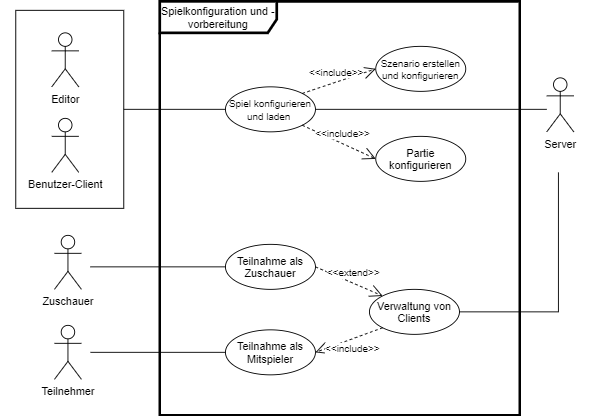
\includegraphics[width=\textwidth]{images/Anwendungsfalldiagramm_Konfiguration}
\captionof{figure}{Anwendungsfalldiagramm für die Anwendungsfälle bei der Konfiguration und Vorbereitung eines Spieles bzw. einer Partie}
\label{fig:use-case-config}
\flushleft

\vspace{2cm}

Die Akteure \rref{A-Benutzer-Client} und \rref{A-Editor} wurden gruppiert, um deutlich zu machen, dass der Editor ein Teil des Benutzer-Clients ist. Denn die Anwender des Spiels nutzen den Editor im Benutzer-Client, um das Spiel zu konfigurieren, wodurch beide Akteure gleichermaßen benötigt werden. \\ Wie man in dem Anwendungsfalldiagramm \autoref{fig:use-case-config} sieht, inkludiert der Anwendungsfall \textit{Spiel konfigurieren} die Anwendungsfälle \textit{Szenario erstellen und konfigurieren} sowie \textit{Partie konfigurieren} und wird durch \textit{Partie- und Szenariokonfiguration laden} erweitert. Diese Gruppenbeziehung besteht so, weil bevor der Server die Konfiguration laden kann, müssen das Szenario und die Partie zunächst konfiguriert werden, weil der Server sonst das Spiel nicht starten kann. Da beide Konfigurationen notwendig sind, müssen sie ablaufen, bevor der Server die Konfiguration laden kann und somit der Anwendungsfall \textit{Spiel konfigurieren} abgeschlossen wird. Die Konfigurationen müssen jedoch nicht geladen werden, da sie auch noch konfiguriert werden können, weswegen dieser Anwendungsfall nur erweitert.\\ Wie den funktionalen Anforderungen zu entnehmen ist, hat der Server die Aufgabe, die Clients zu verwalten, weswegen der Anwendungsfall \textit{Verwaltung von Clients} mit dem Server verbunden ist. Dabei sind, um das Spiel anschließend auch spielen zu können, Mitspieler notwendig. Daher inkludiert \textit{Verwaltung von Clients} den Anwendungsfall \textit{Teilnahme als Mitspieler}. Die Tatsache, dass für den Server zwei Mitspieler notwendig sind, lässt sich jedoch nicht darstellen. Außerdem erlaubt der Server, dass Zuschauer der Partie beitreten und über den Spielablauf informiert werden. Deswegen gibt es einen Anwendungsfall \textit{Teilnahme als Zuschauer}, der \textit{Verwaltung von Clients} extended. Das wird damit begründet, dass Zuschauer teilnehmen können, jedoch kein Teilnehmer einer Partie bewohnen muss, das heißt dieser Anwendungsfall optional ausgeführt wird. 

\centering
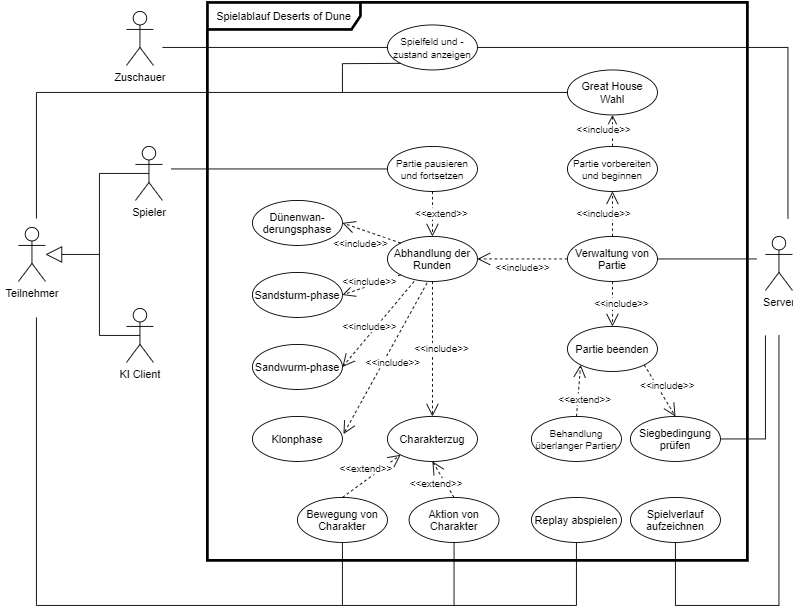
\includegraphics[width=\textwidth]{images/Anwendungsfalldiagramm_Spielablauf}
\captionof{figure}{Anwendungsfalldiagramm für die Anwendungsfälle Spielablaufs von \textsc{DUNE}}
\label{fig:use-case-gameflow}

\flushleft

Dieses Anwendungsfalldiagramm \autoref{fig:use-case-gameflow} behandelt alle Anwendungsfälle, die mit der Spieldurchführung zu tun haben. Dabei gibt es Anwendungsfälle, die nur von dem Akteur \rref{A-Spieler} ausgeführt werden und manche, die auch vom Akteur \rref{A-KI-Client} und damit allgemein dem Mitspieler bzw. Teilnehmer ausgeführt werden. Daher sind Spieler und KI Client Spezialisierung des Teilnehmers. \\ Wie in den funktionalen Anforderungen definiert wurde, hat der Server ebenso die Aufgabe, die Partie zu verwalten. Das heißt, er hat die Aufgabe, die Partie vorzubereiten, zu beginnen, durchzuführen und anschließend auch zu beenden. Um diese Logik darzustellen, gibt es einen Anwendungsfall \textit{Verwaltung von Partie} der \textit{Partie vorbereiten und beginnen}, \textit{Abhandlung der Runden} (= Spieldurchführung) und \textit{Partie beenden} inkludiert, weil alle diese Anwendungsfälle ausgeführt werden müssen, um eine Partie abzuhandeln und zu verwalten. \\ Da die Partievorbereitung die Great-House Wahl beinhaltet, wird \textit{Great House Wahl} von \textit{Partie vorbereiten und beginnen} inkludiert. \\ Die Abhandlung der Runden, das heißt die Durchführung von einem Rundenzyklus beinhaltet die Durchführung der in den Anforderungen definierten Runden. Das heißt, dass zur Abhandlung einer Runde die Anwendungsfälle \textit{Dünenwanderungsphase}, \textit{Sandsturmphase}, \textit{Sandwurmphase}, \textit{Klonphase} und \textit{Charakterzugphase} voraussetzt, weswegen diese inkludiert werden. \\ Der \textit{Charakterzug} wiederum besteht aus Zugphasen, die entweder eine Bewegung oder eine Aktion eines Charakters beinhalten. Da der Charakter sich nicht bewegen muss und auch keine Aktion ausführen muss und damit keiner der beiden Fälle Voraussetzung für einen Charakterzug ist, extenden die Anwendungsfälle \textit{Bewegung von Charakter} und \textit{Aktion von Charakter} \textit{Charakterzug}. \\ Ein ähnliches Argument begründet, warum \textit{Behandlung überlanger Partien} den Fall \textit{Partie beenden} extended. Da nicht unbedingt eine überlange Partie auftreten muss, muss dieser Anwendungsfall nicht unbedingt umgesetzt werden. In jedem Fall muss der Server jedoch die Siegbedingung prüfen\footnote{Bei der Behandlung überlanger Partien sieht diese Siegbedingung zwar anders aus, jedoch wird auch auf eine Siegbedingung geprüft.}, das heißt der Anwendungsfall \textit{Siegbedingung prüfen} muss von dem Fall \textit{Partie beenden} inkludiert werden. \par \par 

Bei dem Anwendungsfalldiagramm \autoref{fig:use-case-config} sind den Anwendungsfällen folgende funktionalen Anforderungen aus \autoref{ssec:fas} zugeordnet: 

\vspace{0.5cm}

\begin{tabularx}{\linewidth}{l|X}
	\textbf{Anwendungsfall} & \textbf{zugeordnete Anforderungen} \\
	\hline
	Spiel konfigurieren und laden & \mfaref{FA-Editor}, \mfaref{FA-Server-Partie-Konfiguration}, \mfaref{FA-ServerlädtSzenario} \\
	Szenario erstellen und konfigurieren & \mfaref{FA-Spielbrett-Erstellung}, \mfaref{FA-Konfiguration}-\mfaref{FA-LadenUndModifizieren}, \mfaref{FA-Szenariokonfiguration}-\mfaref{FA-ZufälligeSzenariokonfiguration} \\
	Partie konfigurieren & \mfaref{FA-Partiekonfiguration}, \mfaref{FA-Parameter-Partiekonfiguration} \\
	Teilnahme als Zuschauer & \mfaref{FA-BC}, \mfaref{FA-Server-Erlaube-Zuschauer}, \mfaref{FA-Registrierung-Zuschauer} \\
	Teilnahme als Mitspieler & \mfaref{FA-BC}, \mfaref{FA-KI}, \mfaref{FA-Registrierung-Spieler}, \mfaref{FA-Verbindungsaufbau-BC}, \mfaref{FA-Start-KI}, \mfaref{FA-Verbindungsaufbau-KI}, \mfaref{FA-Einbindung-KI}, \\
	Verwaltung von Clients & \mfaref{FA-Server}, \mfaref{FA-Spieleranzahl}, \mfaref{FA-Beobachtung}, \mfaref{FA-BC}, \mfaref{FA-Server-Clientverbindung} \\ 
\end{tabularx}

\vspace{0.5cm}

Bei dem Anwendungsfalldigramm \autoref{fig:use-case-gameflow} sind den Anwendungsfällen folgende funktionalen Anforderungen aus \autoref{ssec:fas} zugeordnet: 

\vspace{0.5cm}


\begin{tabularx}{\linewidth}{l|X}
	\textbf{Anwendungsfall} & \textbf{zugeordnete Anforderungen} \\
	\hline
	Spielfeld und -zustand anzeigen & \mfaref{FA-Sichtbarkeit-Spielfeld}-\mfaref{FA-Spielbrett}, \mfaref{FA-Feld}-\mfaref{FA-Feldart-Gebirge}, \mfaref{FA-Server-Information-Spielzustand}, \mfaref{FA-Visualisierung-Spiel}-\mfaref{FA-Visualisierungsdauer} \\
	Great House Wahl & \mfaref{FA-GreatHouses}-\mfaref{FA-Haus-Vernius}, \mfaref{FA-Wahl-GreatHouses} \\ 
	Partie vorbereiten und beginnen & \mfaref{FA-Partievorbereitung}, \mfaref{FA-Beginn einer Partie}, \mfaref{FA-Server-Partiebeginn}, \\ 
	Verwaltung von Partie & \mfaref{FA-Server} \\
	Partie beenden & \mfaref{FA-Partieende} \\
	Siegbedingung prüfen & \mfaref{FA-Partieende}, \mfaref{FA-Siegmetrik}, \mfaref{FA-Server-Siegbedingung},  \\
	Behandlung überlanger Partien & \mfaref{FA-Behandlung-überlanger-Partien}-\mfaref{FA-Phase-Shai-Hulud} \\
	Abhandlung der Runden & \mfaref{FA-Aktion-Spice-Blow}, \mfaref{FA-Runden und Züge} \\ 
	Partie pausieren und fortsetzen & \mfaref{FA-Server-Partiepause}, \mfaref{FA-Pausierung-BC}, \mfaref{FA-Pausierung-KI},\\ 
	Dünenwanderungsphase & \mfaref{FA-Dünenwanderung}, \mfaref{FA-Phase-Dünenwanderung}, \mfaref{FA-Zellulärer-Automat} \\ 
	Sandsturmphase & \mfaref{FA-Sandsturm}, \mfaref{FA-Phase-Sandsturm} \\ 
	Sandwurmphase & \mfaref{FA-Sandwurm}, \mfaref{FA-Phase-Sandwurm}\\ 
	Klonphase & \mfaref{FA-Phase-Klon} \\ 
	Charakterzug & \mfaref{FA-Charaktere}-\mfaref{FA-Stärken-Schwächen-Charaktere}, \mfaref{FA-Spice-Streuung}, \mfaref{FA-Charakterzug-Rundenphase}, \mfaref{FA-Charakterzug}, \mfaref{FA-Server-Verbindungstrennung}-\mfaref{FA-Server-verspätete-Nachrichten}, \mfaref{FA-Server-Session-offen-halten}, \mfaref{FA-Server-Protokollverletzung}, \mfaref{FA-Spielinteraktion}, \mfaref{FA-Vereinfachung-Spielinteraktion}, \mfaref{FA-Zugwahl-KI}-\mfaref{FA-Intelligenzstufen},\\ 
	Bewegung von Charakter & \mfaref{FA-Abstand-Felder}, \mfaref{FA-Bewegung-Charakter}, \mfaref{FA-Spicelieferung-Charakter}, \mfaref{FA-Suche-Nachbarfeld}, \mfaref{FA-gleichwertige-Alternativen}, \\ 
	Aktion von Charakter & \mfaref{FA-Aktionen}-\mfaref{FA-Aktion-Sword-Spin}\\ 
	Spielverlauf aufzeichnen & \mfaref{FA-ReplayLog}\\ 
	Replay abspielen & \mfaref{FA-Replay} \\
	
\end{tabularx}

\vspace{0.5cm}

Die funktionalen Anforderungen \mfaref{FA-Architektur}-\mfaref{FA-Kombinierbarkeit-Komponenten}, \mfaref{FA-Netzwerkprotokoll}-\mfaref{FA-Spielprotokoll} und \mfaref{FA-Docker-Server} finden sich nicht in den Tabellen wieder, da sich nicht eindeutig einem Anwendungsfall zuzuordnen sind. Die Anwendungsfälle \mfaref{FA-Architektur}-\mfaref{FA-Kombinierbarkeit-Komponenten}, die sich mit der Architektur befassen finden sich in den gesamten Anwendungsfalldiagrammen \autoref{fig:use-case-gameflow} und \autoref{fig:use-case-config} wieder durch die Aufteilung der Anwendungsfälle auf die Akteure. \\ Die funktionalen Anforderungen \mfaref{FA-Netzwerkprotokoll}-\mfaref{FA-Spielprotokoll}, die sich mit der Netzwerkkommunikation befassen können allen Anwendungsfällen zugeordnet werden, die etwas mit der Netzwerkkommunikation zu tun haben, wie zum Beispiel \textit{Spielfeld und -zustand anzeigen} oder \textit{Aktion von Charakter}. \\ Die Anforderung \mfaref{FA-Docker-Server} ist eine Anforderung, die sich ebenfalls nicht eindeutig zuordnen lässt, da die Diagramme voraussetzen, dass Server und Benutzer-Client laufen und bereits gestartet wurden, weswegen diese Anforderungen ebenso nicht dargestellt werden kann. \par \par 
Im Folgenden \autoref{ssec:fas} werden die Abläufe und Vorgänge der Anwendungsfälle genauer spezifiziert. 

\subsubsection{Abläufe}
\label{ssec:processes}

Die folgenden Aktivitäts- und Sequenzdiagramme veranschaulichen die Abläufe der einzelnen Anwendungsfälle aus \autoref{sssec:use-cases} und damit die wichtigen Abläufe vor und während des Spiels bzw. Systems

\begin{center}
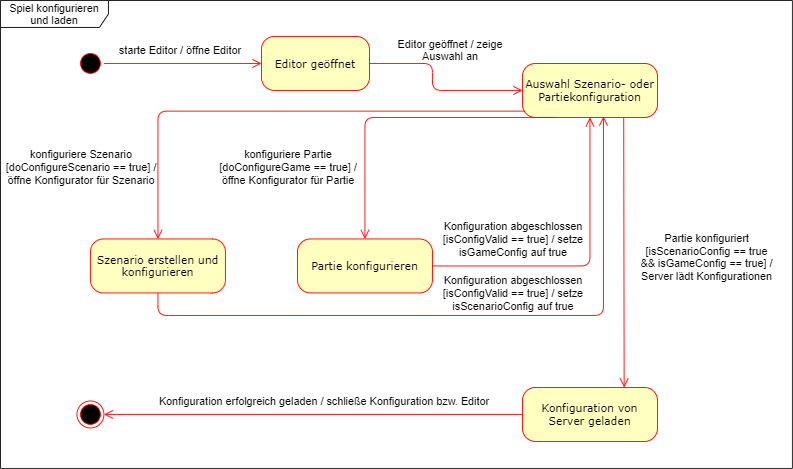
\includegraphics[width=0.85\textwidth]{images/Spiel_konfigurieren}
\captionof{figure}{Zustandsdiagramm für den Ablauf der Konfiguration eines Spiels und dem anschließenden Laden der Konfiguration durch den Server}
\end{center}

\begin{center}
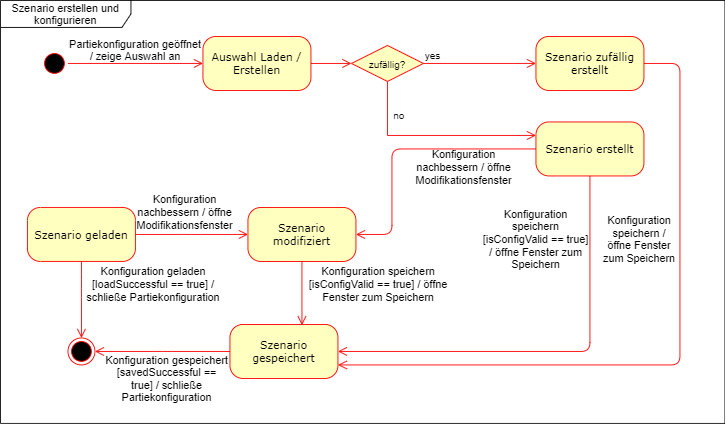
\includegraphics[width=\textwidth]{images/Szenario_konfigurieren}
\captionof{figure}{Zustandsdiagramm für das erstellen, modifizieren und laden von einer Szenariokonfiguration}
\end{center}

\begin{center}
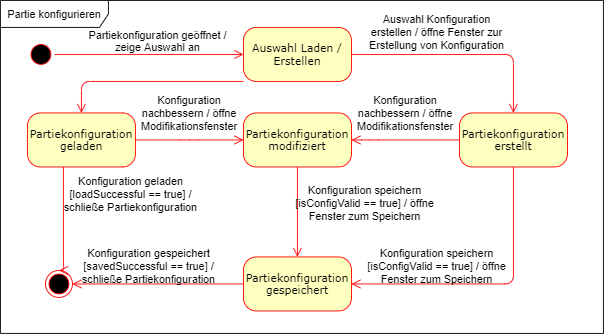
\includegraphics[width=\textwidth]{images/Partie_konfigurieren}
\captionof{figure}{Zustandsdiagramm für das erstellen, modifizieren und laden von einer Partiekonfiguration}
\end{center}

\begin{center}
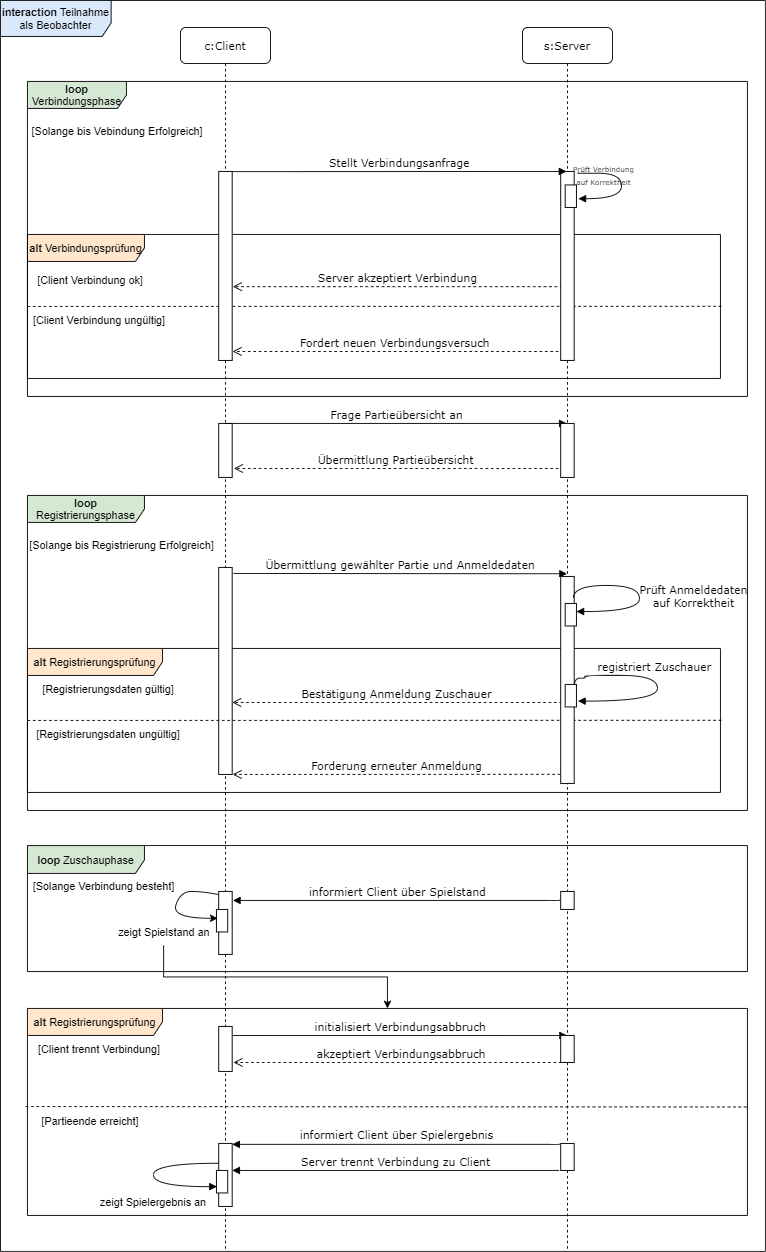
\includegraphics[width=0.85\textwidth]{images/Teilnahme_als_Beobachter}
\captionof{figure}{Sequenzdiagramm für Ablauf der Teilnahme eines Clients als Zuschauer}
\end{center}

\begin{center}
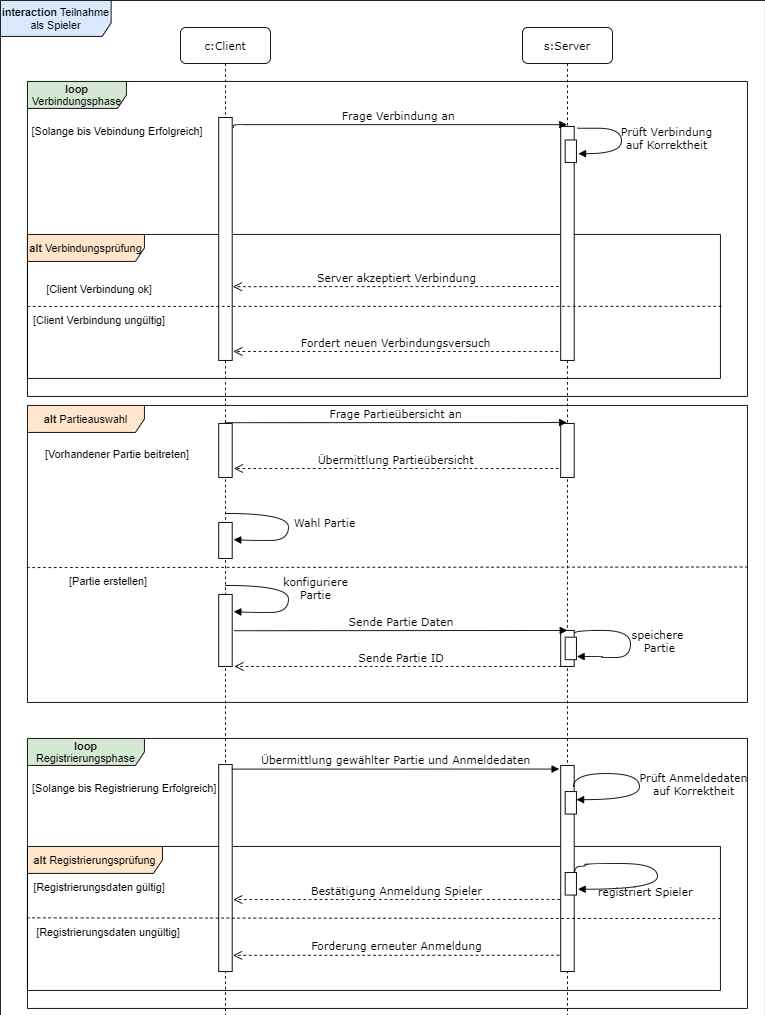
\includegraphics[width=0.85\textwidth]{images/Teilnahme_als_Spieler2} \\ 
...
\end{center}

\begin{center}
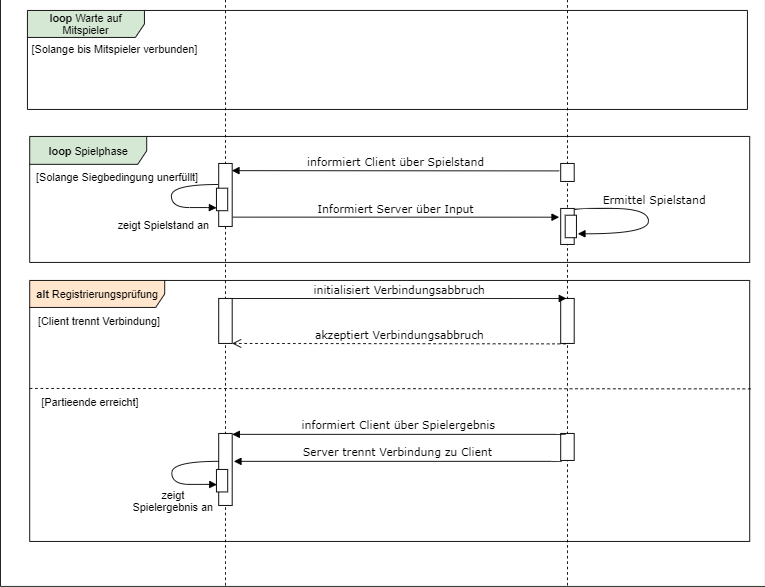
\includegraphics[width=0.85\textwidth]{images/Teilnahme_als_Spieler}
\captionof{figure}{Sequenzdiagramm für Ablauf der Teilnahme eines Clients als Mitspieler (Fortsetzung auf nächster Seite)}
\end{center}

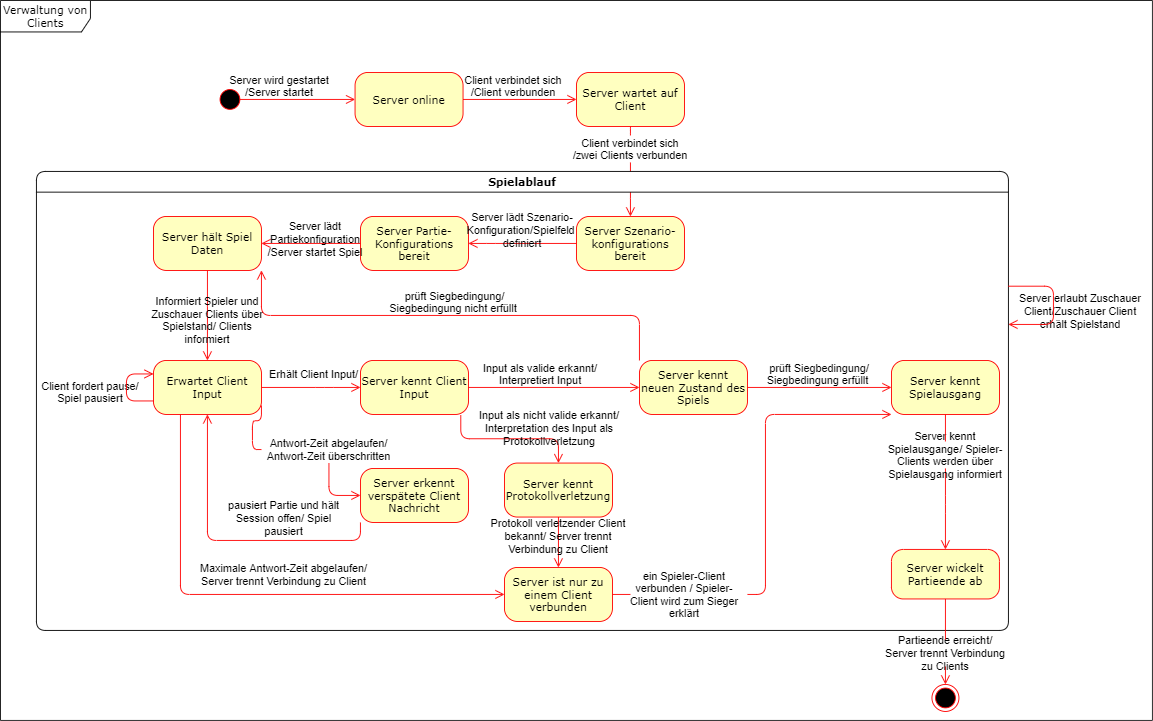
\includegraphics[width=\textwidth]{images/Verwaltung_von_Clients}
\captionof{figure}{Zustandsdiagramm für die Verwaltung von Clients seitens des Servers}

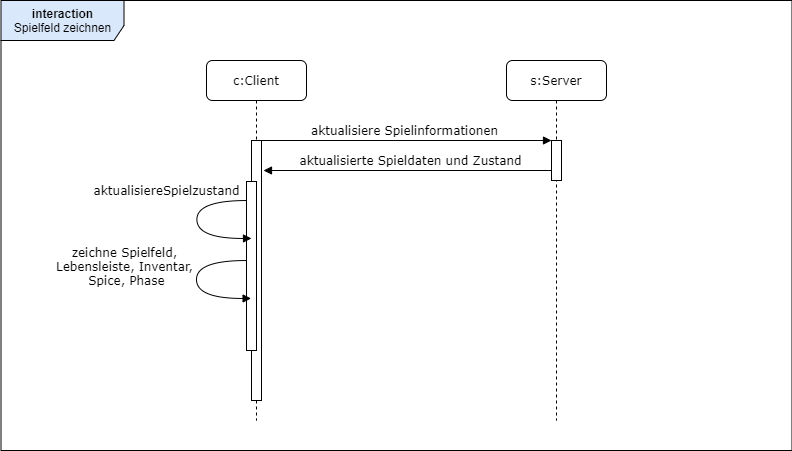
\includegraphics[width=\textwidth]{images/SQ_Spielfeld}
\captionof{figure}{Sequenzdiagramm für Aktualisierung des Servers und Anzeige des neuen Spielstands auf dem Benutzer-Client}


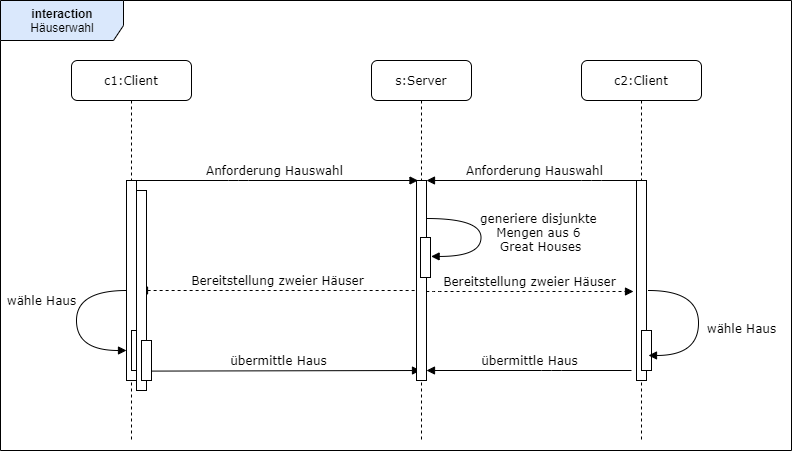
\includegraphics[width=\textwidth]{images/SQ_Hauswahl}
\captionof{figure}{Sequenzdiagramm für die Great House Wahl vor Partiebeginn}

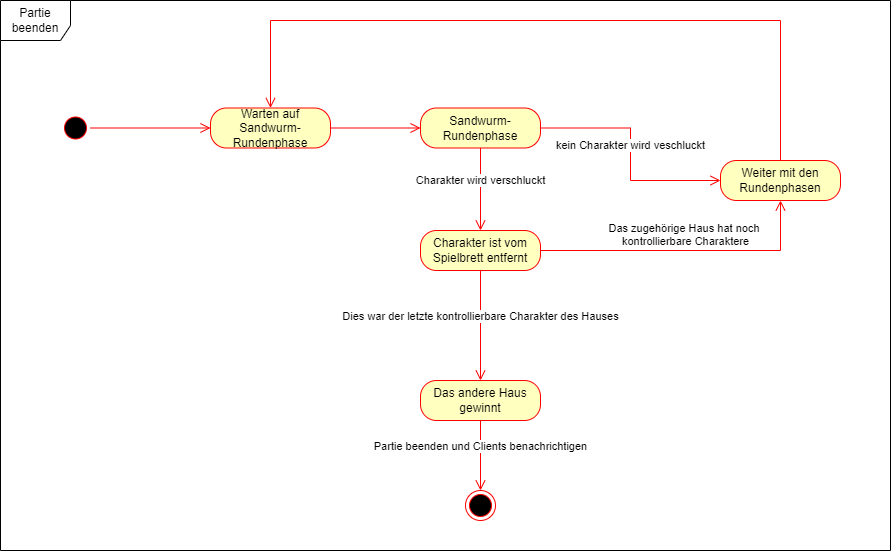
\includegraphics[width=\textwidth]{images/Partie_beenden_Zustandsdiagramm}
\captionof{figure}{Zustandsdiagramm für Beenden der Partie}

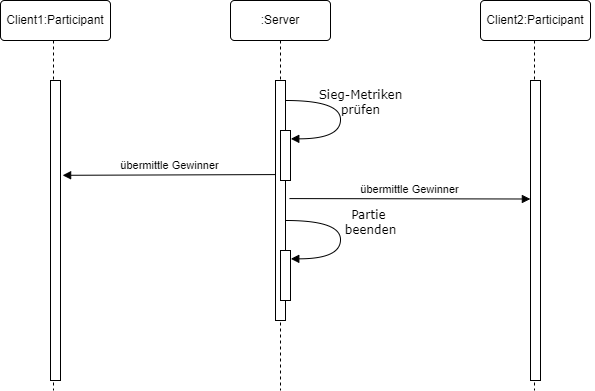
\includegraphics[width=\textwidth]{images/Partie_beenden_Sequenzdiagramm}
\captionof{figure}{Sequenzdiagramm für Beenden der Partie}

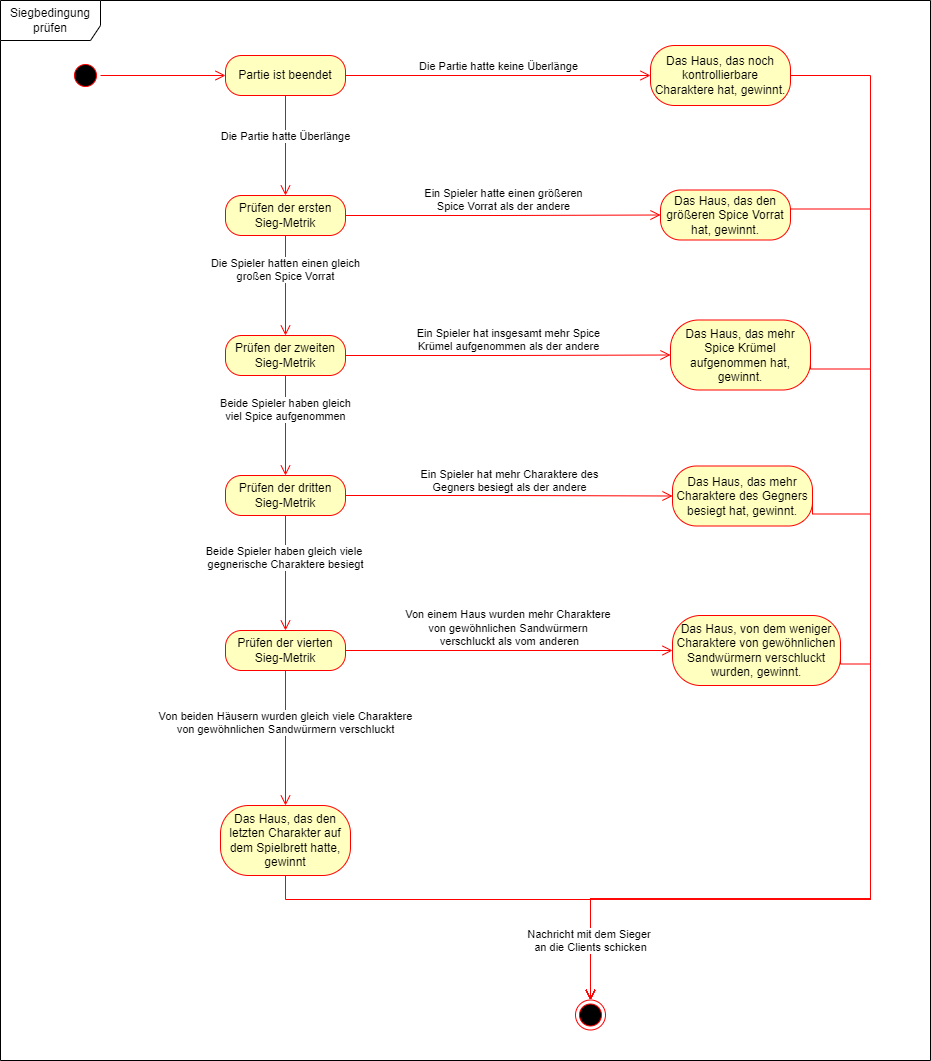
\includegraphics[width=\textwidth]{images/Siegbedingung_pruefen_Zustandsdiagramm}
\captionof{figure}{Zustandsdiagramm für Prüfen der Siegbedingungen}

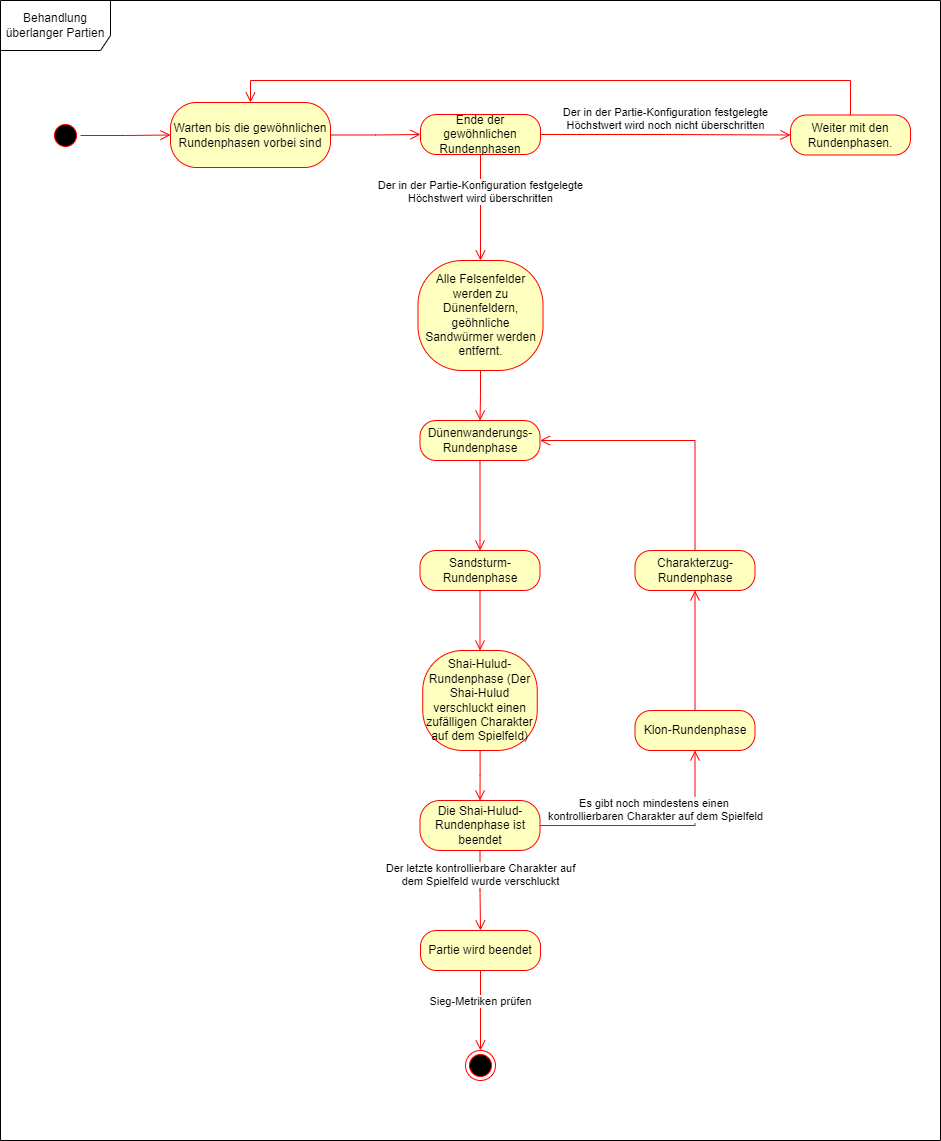
\includegraphics[width=\textwidth]{images/Behandlung_ueberlanger_Partien_Zustandsdiagramm}
\captionof{figure}{Zustandsdiagramm für Behandlung überlanger Partien}

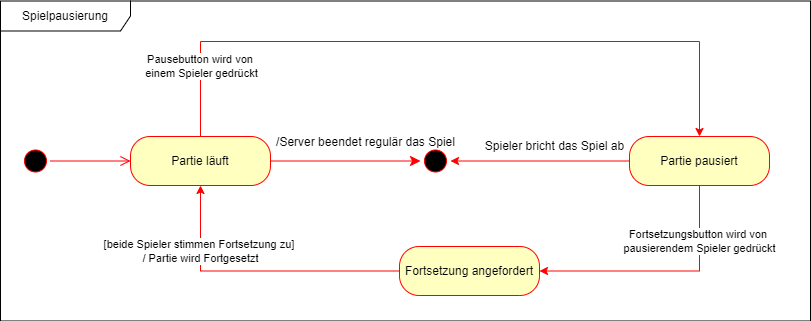
\includegraphics[width=\textwidth]{images/Partie_pausieren}
\captionof{figure}{Zustandsdiagramm für den Ablauf eines Pausierungs- und Wiederaufnahmeantrags für eine Partie von einem menschlichen Benutzer}

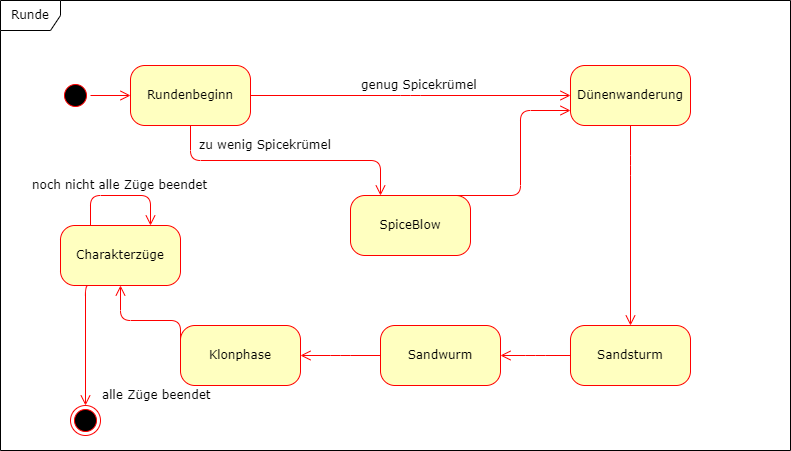
\includegraphics[width=\textwidth]{images/Zustandsdiagramm_Rundenphasen.drawio}
\captionof{figure}{Zustandsdiagramm für den Anwendungsfall Abhandlung der Runde}
\label{fig:state-mashine-round}

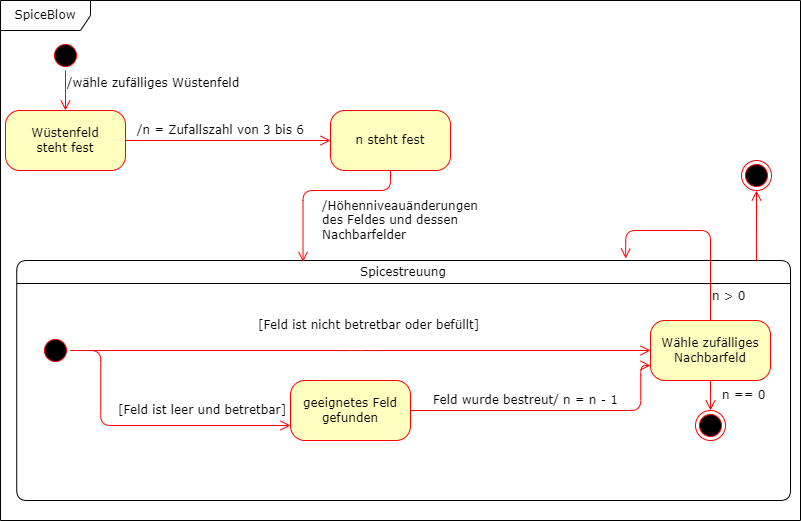
\includegraphics[width=\textwidth]{images/Zustandsdiagramm_SpiceBlow.drawio}
\captionof{figure}{Zustandsdiagramm für den Anwendungsfall SpiceBlow}
\label{fig:state-mashine-spiceblow}

\includegraphics[width=\textwidth]{images/Zustandsdiagramm_Dünenwanderung.drawio}
\captionof{figure}{Zustandsdiagramm für den Anwendungsfall Dünenwanderung}
\label{fig:state-mashine-dunechanging}

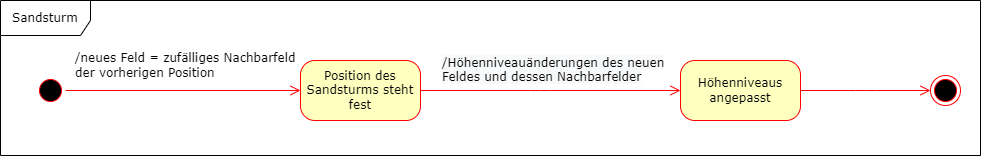
\includegraphics[width=\textwidth]{images/Zustandsdiagramm_SandSturm.drawio}
\captionof{figure}{Zustandsdiagramm für den Anwendungsfall Sandsturm}
\label{fig:state-mashine-sandstorm}

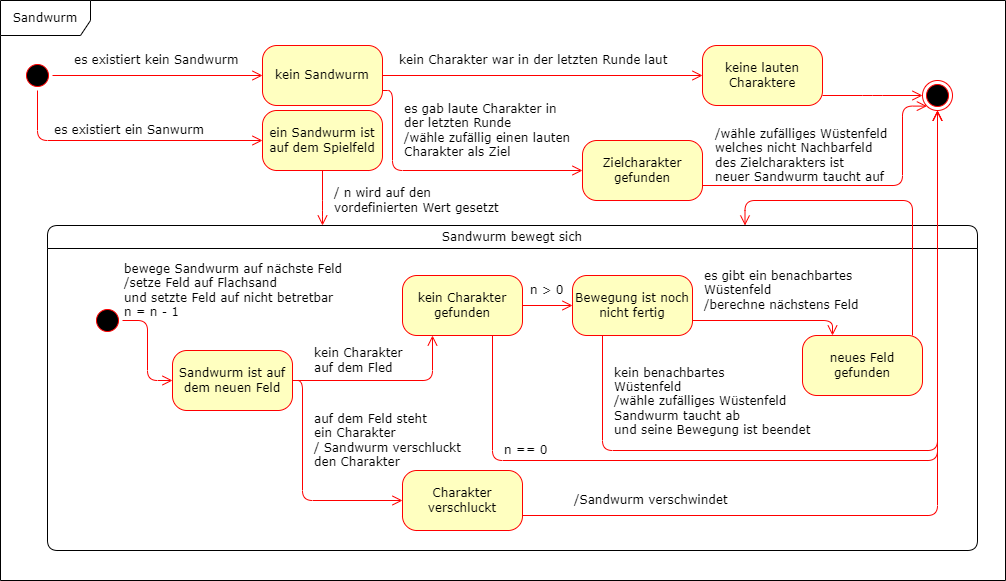
\includegraphics[width=\textwidth]{images/Zustandsdiagramm_SandWurm.drawio}
\captionof{figure}{Zustandsdiagramm für den Anwendungsfall Sandwurm}
\label{fig:state-mashine-sandworm}

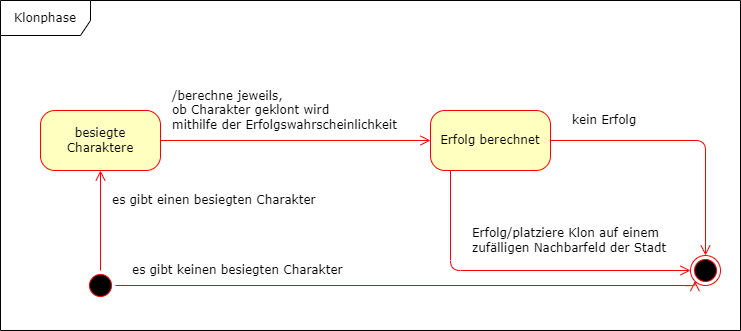
\includegraphics[width=\textwidth]{images/Zustandsdiagramm_Klonphase.drawio}
\captionof{figure}{Zustandsdiagramm für den Anwendungsfall Klonphase}
\label{fig:state-mashine-clonephase}

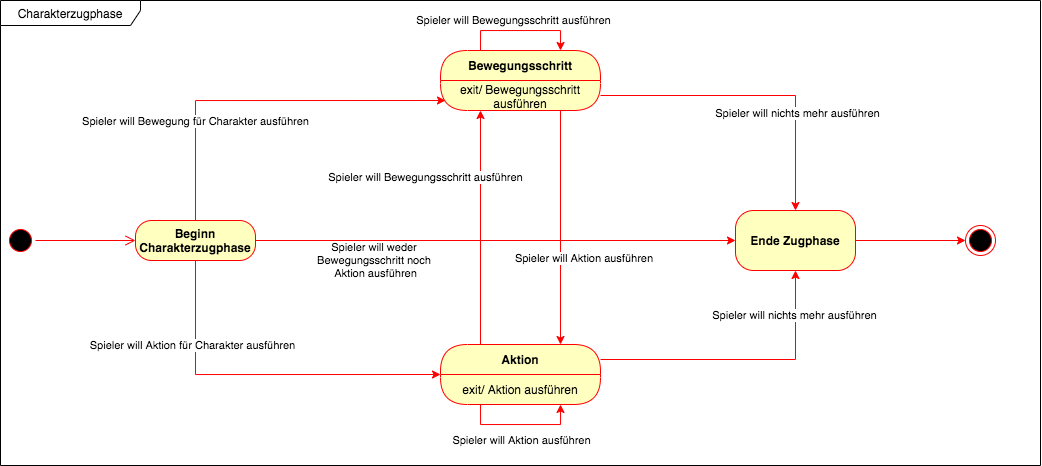
\includegraphics[width=\textwidth]{images/Charakterzugphase}
\captionof{figure}{Zustandsdiagramm für den Ablauf der Phase des Charakterzugs}

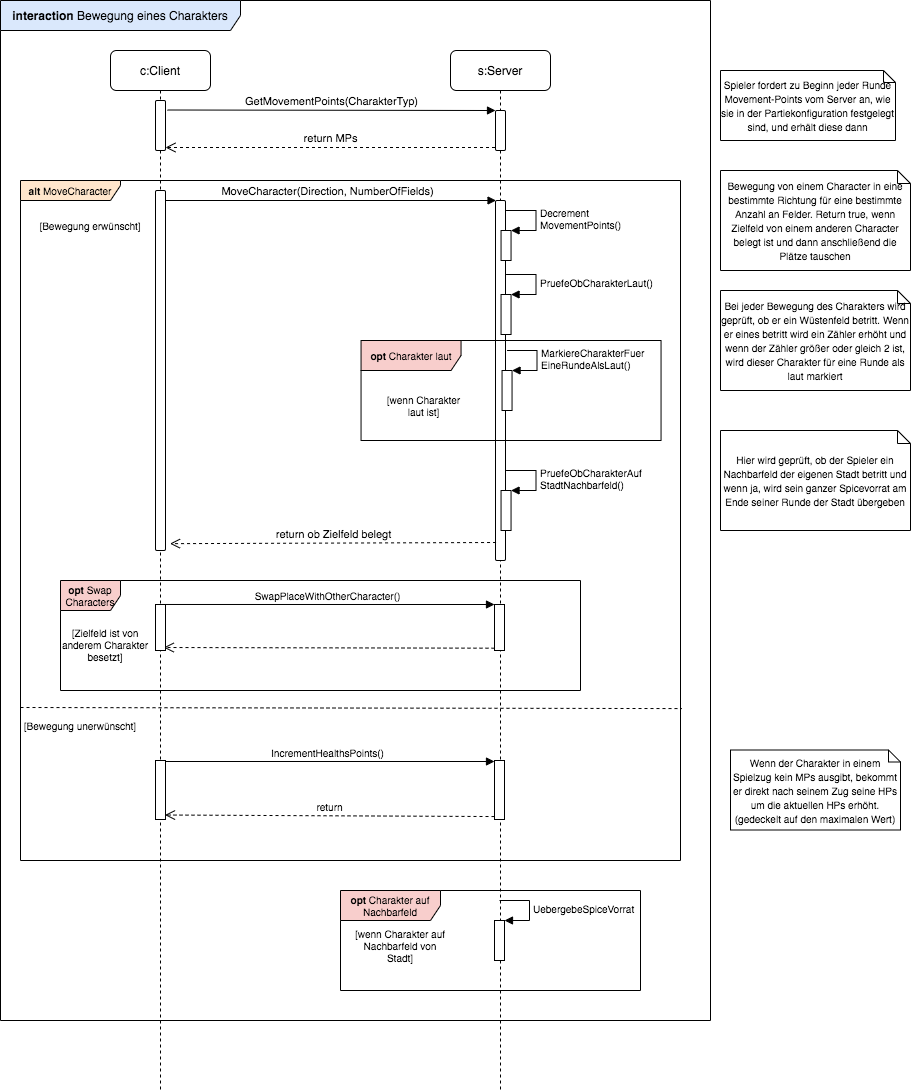
\includegraphics[width=\textwidth]{images/Bewegung_von_Charakter}
\captionof{figure}{Sequenzdiagramm für den Vorgang, wenn ein Charakter bewegt werden soll}

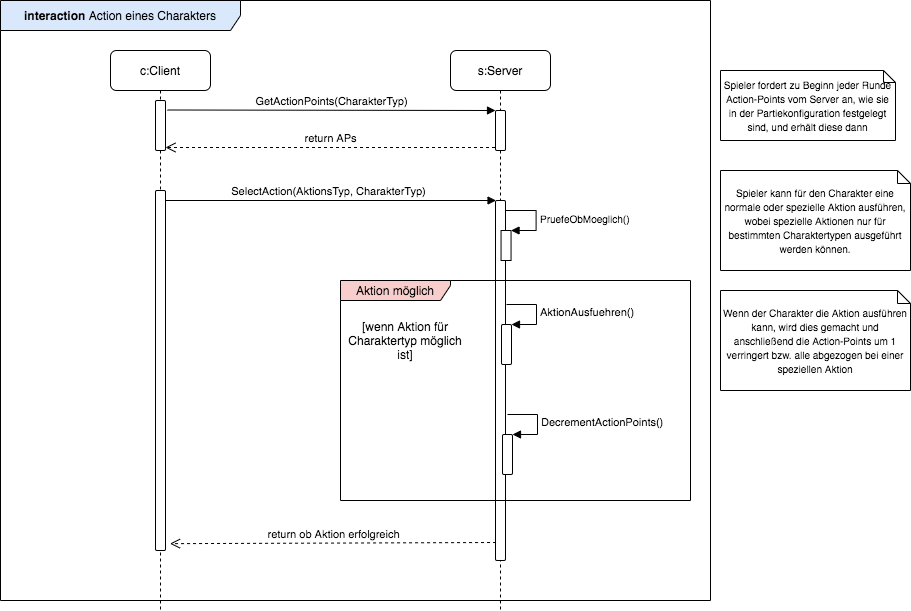
\includegraphics[width=\textwidth]{images/Aktion_von_Charakter}
\captionof{figure}{Sequenzdiagramm für den Vorgang, wenn ein Charakter eine Aktion ausführen soll}

\subsection{Funktionale Anforderungen}
\label{ssec:fas}

Dieser Abschnitt enthält alle funktionalen Systemanforderungen, die die grundlegenden Aktionen des Softwaresystems
spezifizieren. \\ Dabei gilt für die Priorisierung, dass eine Anforderung eine Priorität von 1 (sehr gering, kann) bis 5 (essenziell wichtig, muss unbedingt) bekommen kann. 

\subsubsection*{Komponenten und Architektur}
\fa{Architektur}{Das Spiel \textsc{Deserts of Dune} ist eine verteilte Anwendung mit der Client-Server-Architektur.}{Damit hat man das Spiel in Instanzen aufteilen, die das Spiel bereit stellen und organisieren und Instanzen, die es spielen. Außerdem können somit zwei Spieler auf unterschiedlichen Systemen gegeneinander spielen}{\faref{FA-Spielkomponenten}}{5}{\rref{A-Tutor}}{FA-Architektur}

\fa{Komponenten des Spiels}{Das gesamte System besteht aus vier Komponenten: Server, Benutzer-Client, KI-Client und Editor}{Die Spiellogik soll in diese vier Komponenten aufgeteilt werden als Vorgabe vom Auftraggeber}{\faref{FA-Kombinierbarkeit-Komponenten}, \faref{FA-Server}, \faref{FA-BC}, \faref{FA-KI}, \faref{FA-Editor}}{5}{\rref{A-Tutor}}{FA-Spielkomponenten}

\fa{Server}{Der Server hält die Anwendungslogik zur Verwaltung von Clients, Partien und zur Umsetzung der Spielregeln.}{Der Server soll die gesamte Partie managen und abwickeln, weil diese Aufgabe zentral erledigt werden soll.}{}{5}{\rref{A-Tutor}, \rref{A-Benutzer}, \rref{A-Teilnehmer}}{FA-Server}

\fa{Benutzer-Client}{Der Benutzer-Client ermöglicht es einem einzelnen menschlichen Benutzer, als Spieler oder als Zuschauer an einer Partie teilzuhaben.}{Der Benutzer braucht eine Anwendung, um eine Partie zu verfolgen oder daran teilzunehmen}{\faref{FA-Registrierung-Spieler}, \faref{FA-Registrierung-Zuschauer}}{5}{\rref{A-Tutor}, \rref{A-Benutzer}}{FA-BC}

\fa{Teilnehmeranzahl an Partie}{Es nehmen genau zwei gegeneinander spielende Spieler an einer Partie teil.}{Das Spiel ist darauf ausgerichtet, dass immer zwei Spieler gegeneinander spielen.}{}{5}{\rref{A-Tutor}}{FA-Spieleranzahl}

\fa{Beobachten von Partien}{Das Spiel kann von beliebig vielen Benutzer-Clients beobachtet werden.}{Es soll möglich sein ein beliebiges Spiel zu beobachten.}{\faref{FA-Registrierung-Zuschauer}}{5}{\rref{A-Tutor}, \rref{A-Benutzer}}{FA-Beobachtung}


\fa{KI-Client}{Der KI-Client wird autonom durch eine Künstliche Intelligenz gesteuert und kann als Mitspieler an einer Partie teilnehmen.}{Um auch einzelnen Benutzer ein spannendes Multiplayer-Erlebnis bieten zu können muss es einen KI-Client geben, welcher gegen diese Benutzer antreten kann.}{}{5}{\rref{A-Tutor}, \rref{A-Benutzer}}{FA-KI}

\fa{Editor}{Mit dem Editor kann der Spieler das Spiel konfigurieren}{Dem Nutzer muss es möglich sein, die Konfiguration für ein Spiel anzupassen.}{\faref{FA-Partiekonfiguration}, \faref{FA-Szenariokonfiguration}, \faref{FA-Konfiguration}}{5}{\rref{A-Tutor}, \rref{A-Benutzer}}{FA-Editor}

\subsubsection*{Netzwerkkommunikation und Nachrichtenprotokoll}
\fa{Netzwerkprotokoll}{Die Komponenten verwenden für die Kommunikation untereinander ein Netzwerkprotokoll. Das Netzwerkprotokoll ist ein WebSocket-Protokoll.}{Die Komponenten müssen nach einem Standard kommunizieren und das WebSocket-Protokoll ist ein etabliertes, gut funktionierendes Protokoll}{\faref{FA-Kodierung}}{5}{\rref{A-Tutor}, \rref{A-Entwickler}}{FA-Netzwerkprotokoll}

\fa{Kodierung der Netzwerknachrichten}{Die über die WebSocket-Verbindung ausgetauschten Textstrings sind im UTF-8 Format kodiert}{Die Textstrings müssen aufgrund des Websocket-Protokoll kodiert werden und UTF-8 ist ein Standardformat}{\faref{FA-Netzwerkprotokoll}}{5}{\rref{A-Tutor}, \rref{A-Entwickler}}{FA-Kodierung}

\fa{Nachrichtenformat des Spielprotokolls}{Die über die WebSocket-Verbindung ausgetauschten Textstrings enthalten die Nachrichten des Spielprotokolls. Diese Nachrichten sind in dem Format JSON formatiert.}{Die Textstrings müssen aufgrund des Websocket-Protokoll kodiert werden und UTF-8 ist ein Standardformat.}{\faref{FA-Netzwerkprotokoll}, \faref{FA-Spielprotokoll}}{5}{\rref{A-Tutor}, \rref{A-Entwickler}}{FA-Nachrichtenformat}

\fa{Spielprotokoll}{Das Spielprotokoll wird durch das Standardisierungskomitee definiert.}{Es muss ein fest definiertes Spielprotokoll verwendet werden, um eine Standardisierung zu erhalten. Dieses Protokoll muss teamübergreifend erstellt werden, da es mehrere Teams verwenden.}{\faref{FA-Netzwerkprotokoll}, \faref{FA-Nachrichtenformat}}{5}{\rref{A-Tutor}, \rref{A-Entwickler}}{FA-Spielprotokoll}

\subsubsection*{Szenarios}

\fa{Sichtbarkeit des Spielfeldes}{Alle Spieler können zu jedem Zeitpunkt das gesamte Spielfeld sehen.}{Die Spieler sollen zu jedem Zeitpunkt des Spiels sämtliche Informationen über den Status des Spiels haben, weil das Spiel ein Spiel mit vollständiger Information sein soll.}{\faref{FA-Spielbrett}}{5}{\rref{A-Tutor}, \rref{A-Benutzer}, \rref{A-Teilnehmer}}{FA-Sichtbarkeit-Spielfeld}

\fa{Sichtbarkeit Zustand und Charakterinventar}{Alle Spieler können zu jedem Zeitpunkt alle Charaktere und deren Inventar sehen.}{Die Spieler sollen zu jedem Zeitpunkt des Spiels sämtliche Informationen über den Status des Spiels haben, weil das Spiel ein Spiel mit vollständiger Information sein soll.}{\faref{FA-Charaktere}}{5}{\rref{A-Tutor}, \rref{A-Benutzer}, \rref{A-Teilnehmer}}{FA-Sichtbarkeit-Inventar}

\fa{Spielbrett}{Das Spielbrett ist ein rechteckiges kartesisches Raster aus $x * y$ Feldern. Dieses Spielbrett inklusive aller Felder und Charakter repräsentiert das Szenario.}{Alle Spielbretter sollen rechteckig sein, weil das die Berechnung von Zügen vereinfacht, und die einzelnen Felder sollen klar unterscheidbar sein.}{\faref{FA-Feld}, \faref{FA-Spielbrett-Erstellung}}{5}{\rref{A-Tutor}, \rref{A-Benutzer}, \rref{A-Teilnehmer}}{FA-Spielbrett}

\fa{Erstellung Spielbrett}{Das Spielbrett wird als Szenarion im Editor erstellt und kann dann vom Server geladen werden}{Das Spielbrett muss irgendwie erstellt oder definiert werden können.}{\faref{FA-Spielbrett}, \faref{FA-Szenariokonfiguration}, \faref{FA-Konfiguration}}{5}{\rref{A-Tutor}, \rref{A-Benutzer}, \rref{A-Teilnehmer}}{FA-Spielbrett-Erstellung}

\fa{Feld}{Ein Feld ist ein Teil auf dem Spielbrett und wird durch eine Koordinate positioniert.}{Felder auf dem Spielbrett sollen genau einer Koordinate zugeordnet werden.}{\faref{FA-Spielbrett}}{5}{\rref{A-Tutor}, \rref{A-Teilnehmer}}{FA-Feld}

\fa{Eigenschaften von Feldern}{Ein Feld hat die Eigenschaft Feldart, Betretbarkeit und ein Höhenniveau}{Felder müssen spezifische Eigenschaften haben, um den Spielverlauf durch diese Eigenschaften zu beeinflussen.}{\faref{FA-Feld}, \faref{FA-Feldarten}, \faref{FA-Betretbarkeit}, \faref{FA-Höhenniveau}}{5}{\rref{A-Tutor}, \rref{A-Teilnehmer}}{FA-Feld-Eigenschaften}

\fa{Feldeigenschaft Betretbarkeit}{Die Eigenschaft Betretbarkeit besagt, ob ein Charakter ein Feld betreten kann oder nicht. Wenn dieses betretbare Feld durch ein Objekt blockiert ist, dann heißt es \textit{besetzt}, ansonsten heißt es \textit{frei}}{Es muss klar definiert sein, ob ein spezifisches Feld durch einen Charakter betreten werden kann oder nicht und ob es frei ist.}{\faref{FA-Feld-Eigenschaften}}{5}{\rref{A-Tutor}, \rref{A-Teilnehmer}}{FA-Betretbarkeit}

\fa{Feldeigenschaft Höhenniveau}{Die Eigenschaft Höhenniveau gibt an, ob ein Feld \textit{hoch} oder \textit{niedrig} ist.}{Es muss klar definiert sein, ob ein spezifisches Feld hoch oder niedrig ist, was bei der Bewegung und bei den Aktionen von Charakteren ein Rolle spielt}{\faref{FA-Feld-Eigenschaften}}{5}{\rref{A-Tutor}, \rref{A-Teilnehmer}}{FA-Höhenniveau}

\fa{Feldarten}{Es gibt die verschiedenen Feldarten: \textit{Stadt}, \textit{Flachsand}, \textit{Düne}, \textit{Felsplateau}, \textit{Gebirge}. Für jede Feldart sind die Eigenschaften \textit{Betretbarkeit} und \textit{Höhenniveau} definiert.}{Jedes Feld muss eine definierte Feldart und damit einhergehende Parameter haben.}{\faref{FA-Betretbarkeit}, \faref{FA-Höhenniveau}}{5}{\rref{A-Tutor}, \rref{A-Teilnehmer}}{FA-Feldarten}

\fa{Feldart Stadt}{Die Stadt ist ein Spezialfeld. Auf dem Spielbrett gibt es zwei große Städte, Arrakeen
und Carthag. Beiden Spielern gehört jeweils eine davon. Felder mit der Feldart Stadt sind nicht betretbar und haben ein hohes Höhenniveau.}{Jede Feldart hat besondere Eigenschaften und die Parameter müssen wohldefiniert sein.}{\faref{FA-Feldarten}, \faref{FA-Betretbarkeit}, \faref{FA-Höhenniveau}}{5}{\rref{A-Tutor}, \rref{A-Teilnehmer}, \rref{A-Benutzer}}{FA-Feldart-Stadt}

\fa{Feldart Flachsand}{Flachsand ist ein Wüstenfeld, welches flach und niedrig gelegen ist. Felder der Feldart Flachsand sind betretbar und haben ein niedriges Höhenniveau.}{Jede Feldart hat besondere Eigenschaften und die Parameter müssen wohldefiniert sein.}{\faref{FA-Feldarten}, \faref{FA-Betretbarkeit}, \faref{FA-Höhenniveau}}{5}{\rref{A-Tutor}, \rref{A-Teilnehmer}, \rref{A-Benutzer}}{FA-Feldart-Flachsand}

\fa{Feldart Düne}{Die Düne ist ein Wüstenfeld, welches hügelig und höher gelegen ist. Felder der Feldart Düne sind betretbar und haben ein hohes Höhenniveau.}{Jede Feldart hat besondere Eigenschaften und die Parameter müssen wohldefiniert sein.}{\faref{FA-Feldarten}, \faref{FA-Betretbarkeit}, \faref{FA-Höhenniveau}}{5}{\rref{A-Tutor}, \rref{A-Teilnehmer}, \rref{A-Benutzer}}{FA-Feldart-Düne}

\fa{Feldart Felsplateau}{Das Felsplateau ist ein Felsenfeld, welches flach und niedrig gelegen ist. Felder der Feldart Felsplateau sind betretbar und haben ein niedriges Höhenniveau.}{Jede Feldart hat besondere Eigenschaften und die Parameter müssen wohldefiniert sein.}{\faref{FA-Feldarten}, \faref{FA-Betretbarkeit}, \faref{FA-Höhenniveau}}{5}{\rref{A-Tutor}, \rref{A-Teilnehmer}, \rref{A-Benutzer}}{FA-Feldart-Felsplateau}

\fa{Feldart Gebirge}{Das Gebirge ist ein Felsenfeld, welches hoch gelegen und unpassierbar ist. Felder der Feldart Gebirge sind nicht betretbar und haben ein hohes Höhenniveau.}{Jede Feldart hat besondere Eigenschaften und die Parameter müssen wohldefiniert sein.}{\faref{FA-Feldarten}, \faref{FA-Betretbarkeit}, \faref{FA-Höhenniveau}}{5}{\rref{A-Tutor}, \rref{A-Teilnehmer}, \rref{A-Benutzer}}{FA-Feldart-Gebirge}

\fa{Entfernung Felder}{Die Entfernung zwischen zwei Feldern A und B ist definiert als die minimale Anzahl von aufeinanderfolgenden
Schritten auf alle 8 Nachbarfelder (gemäß der Moore Neighborhood-Definition), um von A nach B zu gelangen.}{Der Abstand zwischen Feldern muss klar definiert sein.}{\faref{FA-Feld}}{5}{\rref{A-Tutor}, \rref{A-Entwickler}}{FA-Abstand-Felder}

\subsubsection*{Great Houses}

\fa{Great Houses}{Im Spiel gibt es sechs Great Houses, das heißt große Adelshäuser, die miteinander konkurrieren. Jedes der Häuser hat genau einen Namen und genau eine Farbe und besteht aus
einer Reihe von Charakteren, die bei \faref{FA-Charaktere} genauer beschrieben werden}{Die Great Houses sollen farblich, namentlich und durch die Eigenschaften ihrer Charaktere unterscheidbar sein und dem Spieler Abwechselung bieten und verschiene Strategien in das Spiel bringen.}{\faref{FA-Charaktere}}{5}{\rref{A-Tutor}, \rref{A-Teilnehmer}, \rref{A-Benutzer}}{FA-GreatHouses}

\fa{Haus Corrino}{Dieses Great House hat den Namen \textit{House Corrino}, die Farbe \textit{Gold} und die folgenden Charaktere: Emperor Shaddam IV Corrino (Noble), Princess Irulan Corrino (Bene Gesserit), Count Hasimir Fenring (Mentat), Lady Margot Fenring (Bene Gesserit), Reverend Mother Gaius Helen Mohiam (Bene Gesserit) und Captain Aramsham (Fighter).}{Die Great Houses sollen farblich, namentlich und durch die Eigenschaften ihrer Charaktere unterscheidbar sein.}{\faref{FA-GreatHouses}, \faref{FA-Noble}, \faref{FA-Mentat}, \faref{FA-Bene-Gesserit}, \faref{FA-Fighter}}{5}{\rref{A-Tutor}, \rref{A-Teilnehmer}, \rref{A-Benutzer}}{FA-Haus-Corrino}

\fa{Haus Atreides}{Dieses Great House hat den Namen \textit{House Atreides}, die Farbe \textit{Grün} und die folgenden Charaktere: Duke Leto Atreides (Noble), Paul Atreides (Noble),  Lady Jessica (Bene Gesserit), Thufir Hawat (Mentat), Gurney Halleck (Fighter) und Space Pug, Duke Letos tapferer Mopshund (Fighter).}{Die Great Houses sollen farblich, namentlich und durch die Eigenschaften ihrer Charaktere unterscheidbar sein.}{\faref{FA-GreatHouses}, \faref{FA-Noble}, \faref{FA-Mentat}, \faref{FA-Bene-Gesserit}, \faref{FA-Fighter}}{5}{\rref{A-Tutor}, \rref{A-Teilnehmer}, \rref{A-Benutzer}}{FA-Haus-Atreides}

\fa{Haus Harkonnen}{Dieses Great House hat den Namen \textit{House Harkonnen}, die Farbe \textit{Rot} und die folgenden Charaktere: Baron Vladimir Harkonnen (Noble),  Count Glossu Beast Rabban (Fighter), Feyd-Rautha Rabban (Fighter), Piter De Vries (Mentat), Iakin Nefud (Fighter) und Pet Spider (Fighter).}{Die Great Houses sollen farblich, namentlich und durch die Eigenschaften ihrer Charaktere unterscheidbar sein.}{\faref{FA-GreatHouses}, \faref{FA-Noble}, \faref{FA-Mentat}, \faref{FA-Bene-Gesserit}, \faref{FA-Fighter}}{5}{\rref{A-Tutor}, \rref{A-Teilnehmer}, \rref{A-Benutzer}}{FA-Haus-Harkonnen}

\fa{Haus Ordos}{Dieses Great House hat den Namen \textit{House Ordos}, die Farbe \textit{Blau} und die folgenden Charaktere: Executrix (Noble), The Speaker (Noble), Ammon (Mentat), Edric (Mentat), Roma Atani (Mentat) und Robot (Fighter).}{Die Great Houses sollen farblich, namentlich und durch die Eigenschaften ihrer Charaktere unterscheidbar sein.}{\faref{FA-GreatHouses}, \faref{FA-Noble}, \faref{FA-Mentat}, \faref{FA-Bene-Gesserit}, \faref{FA-Fighter}}{5}{\rref{A-Tutor}, \rref{A-Teilnehmer}, \rref{A-Benutzer}}{FA-Haus-Ordos}

\fa{Haus Richese}{Dieses Great House hat den Namen \textit{House Richese}, die Farbe \textit{Silber} und die folgenden Charaktere: Count Ilban Richese (Noble), Helena Richese (Noble), Haloa Rund (Mentat), Flinto Kinnis (Mentat), Tenu Chobyn (Mentat) und Yresk (Fighter).}{Die Great Houses sollen farblich, namentlich und durch die Eigenschaften ihrer Charaktere unterscheidbar sein.}{\faref{FA-GreatHouses}, \faref{FA-Noble}, \faref{FA-Mentat}, \faref{FA-Bene-Gesserit}, \faref{FA-Fighter}}{5}{\rref{A-Tutor}, \rref{A-Teilnehmer}, \rref{A-Benutzer}}{FA-Haus-Richese}

\fa{Haus Vernius}{Dieses Great House hat den Namen \textit{House Vernius}, die Farbe \textit{Violett} und die folgenden Charaktere: Earl Dominic Vernius (Noble), Lady Shando Vernius (Noble), Kailea Vernius (Noble), Tessia Vernius (Bene Gesserit), Rhombur Vernius (Fighter) und Bronso Vernius (Mentat).}{Die Great Houses sollen farblich, namentlich und durch die Eigenschaften ihrer Charaktere unterscheidbar sein.}{\faref{FA-GreatHouses}, \faref{FA-Noble}, \faref{FA-Mentat}, \faref{FA-Bene-Gesserit}, \faref{FA-Fighter}}{5}{\rref{A-Tutor}, \rref{A-Teilnehmer}, \rref{A-Benutzer}}{FA-Haus-Vernius}

\subsubsection*{Charaktere}

\fa{Charaktere}{Charaktere haben bestimmte Eigenschaften, deren Werte (abhängig vom Charakter-Typ) in der Partiekonfiguration
definiert sind. Sie haben einen \textit{Namen}, ein \textit{Haus}, welchem sie angehören, \textit{Health Points}, \textit{Movement Points}, \textit{Angriffsschaden} und ein \textit{Inventar}. Die Werte und das Inventar aller Charaktere sind für alle Spieler sichtbar.}{Charaktere werden strategisch durch ihre Eigenschaften und deren Werte unterschieden.}{\faref{FA-Partiekonfiguration}, \faref{FA-Sichtbarkeit-Inventar}}{5}{\rref{A-Tutor}, \rref{A-Teilnehmer}, \rref{A-Benutzer}}{FA-Charaktere}

\fa{Eigenschaft Health Points}{Charaktere haben sogenannte Health Points, die angeben, wie viel Schaden der Charakter noch bekommen kann, bevor er stirbt.}{Charaktere brauchen Lebenspunkte, um zu entscheiden, ob sie noch leben oder nicht.}{\faref{FA-Charaktere}}{5}{\rref{A-Tutor}, \rref{A-Teilnehmer}, \rref{A-Benutzer}}{FA-Health-Points}

\fa{Tod eines Charakters}{Wenn der Wert der Health Points eines Charakters auf 0 sinkt, dann ist der Charakter besiegt. Anschließend wird dieser von der Karte entfernt und alle Spicekrümel nach der Spicekrümel-Logik auf dem Spielfeld verteilt.}{Es muss definiert sein, was nach dem Tod eines Charakters inklusive seines Spice passiert.}{\faref{FA-Health-Points}, \faref{FA-Spice-Streuung}}{5}{\rref{A-Tutor}, \rref{A-Teilnehmer}, \rref{A-Benutzer}}{FA-Charakter-Tod}

\fa{Heilung von Health-Points}{Ein Charakter, welcher in seinem Zug keine Movement-Points ausgibt, bekommt am Ende des Zuges seine Health-Points um seine Heilungs-Health Points erhöht.}{ Es muss klar definiert sein, wann ein Charakter sich heilt.}{}{5}{\rref{A-Tutor}, \rref{A-Teilnehmer}}{FA-Heilung-Charakter}

\fa{Charakter-Typen}{Der Charakter-Typ bestimmt die \textit{Health Points}, \textit{Heilungs-Health Points}, \textit{Movement Points}, \textit{Action Points}, \textit{Inventargröße} und den \textit{Angriffsschaden} des Charakters. Zudem ermöglicht der Charakter-Typ, dem Charakter eventuell spezielle Aktionenen ausführen zu können.}{Charaktere werden strategisch durch ihre Eigenschaften und deren Werte unterschieden. }{\faref{FA-Charaktere}, \faref{FA-Spezielle-Aktion}, \faref{FA-Stärken-Schwächen-Charaktere}}{5}{\rref{A-Tutor}, \rref{A-Teilnehmer}, \rref{A-Benutzer}}{FA-Charakter-Typen}

\fa{Charakter-Typ Noble}{Noble ist ein hochwohlgeborenener Adliger. Dafür sind seine Eigenschaften nur durchschnittlich. Die genauen Werte seiner Eigenschaften sind in der Partiekonfiguration zu konfigurieren.}{Die Eigenschaften der Charakter-Typen werden in der Partiekonfiguration konfiguriert und zu einem späteren Zeitpunkt genauer festgelegt, um eine Einfluss-Balance zwischen den Charakter-Typen zu ermöglichen.}{\faref{FA-Charaktere}, \faref{FA-Charakter-Typen}}{5}{\rref{A-Tutor}, \rref{A-Teilnehmer}, \rref{A-Benutzer}}{FA-Noble}


\fa{Charakter-Typ Mentat}{Mentat ist ein Charakter-Typ, der sehr schlau ist, und deshalb besonders effizient darin, Aktionen auszuführen und Spice zu sammeln. Er hält aber im Kampf nicht besonders viel aus. Die genauen Werte der Eigenschaften sind in der Partiekonfiguration zu konfigurieren.}{Die Eigenschaften der Charakter-Typen werden in der Partiekonfiguration konfiguriert und zu einem späteren Zeitpunkt genauer festgelegt, um eine Einfluss-Balance zwischen den Charakter-Typen zu ermöglichen.}{\faref{FA-Charaktere}, \faref{FA-Charakter-Typen}}{5}{\rref{A-Tutor}, \rref{A-Teilnehmer}, \rref{A-Benutzer}}{FA-Mentat}


\fa{Charakter-Typ Bene Gesserit}{Bene Gesserit ist ein Charakter-Typ, der schnell und wendig ist und eine hohe Heilungsrate besitzt. Die genauen Werte der Eigenschaften sind in der Partie-Konfiguration zu konfigurieren.}{Die Eigenschaften der Charakter-Typen werden in der Partiekonfiguration konfiguriert und zu einem späteren Zeitpunkt genauer festgelegt, um eine Einfluss-Balance zwischen den Charakter-Typen zu ermöglichen.}{\faref{FA-Charaktere}, \faref{FA-Charakter-Typen}}{5}{\rref{A-Tutor}, \rref{A-Teilnehmer}, \rref{A-Benutzer}}{FA-Bene-Gesserit}


\fa{Charakter-Typ Fighter}{Fighter ist ein Charakter-Typ, der im Kampf viel Schaden macht und viele Health-Points hat. Die genauen Werte der Eigenschaften sind in der Partiekonfiguration zu konfigurieren.}{Die Eigenschaften der Charakter-Typen werden in der Partiekonfiguration konfiguriert und zu einem späteren Zeitpunkt genauer festgelegt, um eine Einfluss-Balance zwischen den Charakter-Typen zu ermöglichen.}{\faref{FA-Charaktere}, \faref{FA-Charakter-Typen}}{5}{\rref{A-Tutor}, \rref{A-Teilnehmer}, \rref{A-Benutzer}}{FA-Fighter}

\fa{Stärken und Schwächen von Charakter-Typen}{Charakter-Typen haben unterschiedliche Stärken und Schwächen ähnlich dem Schere-Stein-Papier Prinzip.}{Kein Charakter-Typ soll alleine alles gut können, sie sollen sich gegenseitig ergänzen und effektiv gegeneinander sein.}{\faref{FA-Charaktere}}{5}{\rref{A-Tutor}, \rref{A-Teilnehmer}, \rref{A-Benutzer}}{FA-Stärken-Schwächen-Charaktere}

\subsubsection*{Bewegung}

\fa{Bewegung von Charakteren}{Zu Beginn seines Zuges bekommt jeder Charakter so viele Movement Points (MP), wie in der Partiekonfiguration
für seinen Charakter-Typ festgelegt ist. Für einen Movement Point kann sich der Charakter auf ein betretbares Nachbarfeld bewegen.}{Es muss klar definiert sein, wie weit und wohin sich Charaktere jede Runde bewegen dürfen.}{\faref{FA-Charaktere}, \faref{FA-Charakter-Typen}, \faref{FA-Feld}, \faref{FA-Betretbarkeit}, \faref{FA-Bewegungsrichtung-Charakter}}{5}{\rref{A-Tutor}, \rref{A-Teilnehmer}}{FA-Bewegung-Charakter}

\fa{Bewegungsrichtung von Charakteren}{Ein Charakter kann sich in horizontaler, vertikaler oder diagonaler Richtun bewegen.}{Es muss klar definiert sein, in welche Richtungen sich ein Charakter-Typ bewegen darf.}{\faref{FA-Charaktere}, \faref{FA-Charakter-Typen}, \faref{FA-Feld}, \faref{FA-Betretbarkeit}}{5}{\rref{A-Tutor}, \rref{A-Teilnehmer}}{FA-Bewegungsrichtung-Charakter}

\fa{Drängeln von Charakteren}{Bewegt sich ein Charakter auf ein Feld, auf dem bereits ein Charakter steht, tauschen die beiden Charaktere die Felder.}{Die Interaktion zwischen einem Charakter, der bereits auf einem Feld steht und einem zweiten Charakter, welcher das Feld betritt, muss eindeutig definiert sein.}{\faref{FA-Charaktere}, \faref{FA-Charakter-Typen}, \faref{FA-Feld}, \faref{FA-Feldarten}, \faref{FA-Betretbarkeit}}{5}{\rref{A-Tutor}, \rref{A-Teilnehmer}}{FA-Drängeln-Charakter}

\fa{Lautheit in der Wüste}{Am Anfang seines Zuges gilt ein Charakter als leise. Charaktere werden als laut markiert, wenn sie mindestens zweimal aktiv ein Wüstenfeld in einem Zug betreten.}{Es muss klar definiert werden, wann Charaktere als laut markiert werden.}{\faref{FA-Charaktere}}{5}{\rref{A-Tutor}, \rref{A-Teilnehmer}}{FA-Lautheit-Charakter}

\fa{Abliefern von Spice}{Ist ein Charakter auf einem Nachbarfeld seiner Stadt, so wird das Spice aus seinem Inventar direkt der Stadt übergeben und dem Spice-Vorrat des Hauses hinzugezählt. Das heißt der Chatakter hat genau 0 Spice im Inventar und die Stadt genau die Menge mehr, die der Charakter vorher im Inventar hatte.}{Es muss klar geregelt sein, wie Charaktere Spice bei ihrer Stadt abliefern.}{\faref{FA-Charaktere}}{5}{\rref{A-Tutor}, \rref{A-Teilnehmer}}{FA-Spicelieferung-Charakter}

\subsubsection*{Aktionen}

\fa{Aktionen}{Aktionen sind aktive Handlungen, welche Charaktere ausführen können. Das Einsetzen von Aktionen kostet den Charakter immer Action Points, die der Charakter zu Beginn seines Zuges erhält.}{Aktionen sind notwendig, um zu definieren, welche Handlungen welche Charaktere ausführen können.}{\faref{FA-Charaktere}, \faref{FA-Charakter-Typen}}{5}{\rref{A-Tutor}, \rref{A-Teilnehmer}}{FA-Aktionen}

\fa{normale Aktion}{Normale Aktionen können von allen Charakteren ausgeführt werden. Dies ist unabhängig davon, welchen Charakter-Typ ein Charakter hat. Sie kosten den Charakter immer genau einen Action Point. Zu den normalen Aktionen gehören Angriff, Spice aufsammeln und Spice übergeben.}{Normale Aktionen kategorisieren alle Aktionen, welche durch jeden Charakter ausgeführt werden können.}{\faref{FA-Charaktere}, \faref{FA-Charakter-Typen}, \faref{FA-Aktionen}}{5}{\rref{A-Tutor}, \rref{A-Teilnehmer}}{FA-Normale-Aktion}


\fa{Aktion: Angriff}{Mit dieser normalen Aktion kann ein beliebiger Charakter einen gegnerischen Charakter auf einem benachbarten Feld verletzen. Der gegnerische Charakter bekommt, wenn beide Charaktere auf dem gleichen Höhenniveau sind, den Angriffsschaden des Angreifers von seinen Health Points abgezogen. Ist der Angreifer auf einem hohen Feld und der gegnerische Charakter auf einem niedrigen Feld, so bekommt der gegnerische Charakter $frac{4}{3} *$ Angriffsschaden des Angreifers von seinen Health Points abgezogen. Bei gegenteiliger Situation erhält der gegnerische Charakter $\frac{2}{3} *$ Angriffsschaden des Angreifers von seinen Health Points abgezogen.}{Es muss klar definiert sein, wie die Aktion Angriff abläuft, welche Vorbedingungen gelten müssen und welche Auswirkungen sie hat.}{\faref{FA-Charaktere}, \faref{FA-Charakter-Typen}, \faref{FA-Normale-Aktion}, \faref{FA-Höhenniveau}}{5}{\rref{A-Tutor}, \rref{A-Teilnehmer}}{FA-Aktion-Angriff}

\fa{Aktion: Spice aufsammeln}{Ein Charakter kann mit einer Aktion einen Spicekrümel von dem Feld, auf dem er steht, in sein Inventar aufnehmen, sofern dieses nicht voll ist.}{Es muss klar definiert sein, wie die Aktion Spice aufsammeln abläuft, welche Vorbedingungen gelten müssen und welche Auswirkungen sie hat.}{\faref{FA-Charaktere}, \faref{FA-Charakter-Typen}, \faref{FA-Normale-Aktion}, \faref{FA-Höhenniveau}}{5}{\rref{A-Tutor}, \rref{A-Teilnehmer}}{FA-Aktion-Spice-Aufsammeln}

\fa{Aktion: Spice übergeben}{Ein Charakter kann mit einer Aktion eine beliebige Teilmenge der Spicekrümel in seinem Inventar auf das Inventar eines benachbarten verbündeten Charakters übertragen, sofern dieser genügend Platz im Inventar hat.}{Es muss klar definiert sein, wie die Aktion Spice übergeben abläuft, welche Vorbedingungen gelten müssen und welche Auswirkungen sie hat.}{\faref{FA-Charaktere}, \faref{FA-Charakter-Typen}, \faref{FA-Normale-Aktion}}{5}{\rref{A-Tutor}, \rref{A-Teilnehmer}}{FA-Aktion-Spice-Übergeben}

\fa{spezielle Aktion}{Über diese Kategorie von Aktionen verfügen nur spezielle Charakter-Typen. Sie kosten immer die gesamten Action Points, die der Charakter in einer Runde zur Verfügung hat.}{Spezielle Aktionen kategorisieren alle Aktionen, welche nur durch bestimmte Charakter-Typen ausgeführt werden können.}{\faref{FA-Charaktere}, \faref{FA-Charakter-Typen}, \faref{FA-Aktionen}}{5}{\rref{A-Tutor}, \rref{A-Teilnehmer}}{FA-Spezielle-Aktion}


\fa{Aktion: Kanly}{Kanly ist eine spezielle Aktion, welche nur Charaktere vom Charakter-Type Noble ausführen können. Und die nur auf Charaktere vom Charakter-Type Nobel angewendet werden kann. Dies ist ein ritualisierter Angriff zwischen Nobel, welcher das Ziel des Angriffs mit einer Kanly-Erfolgswahrscheinlichkeit, welche in der Partie-Konfiguration festgehalten ist, besiegt. Bei Misserfolg passiert nichts.}{ Es muss klar definiert sein, wie die Aktion Kanly abläuft, welche Vorbedingungen gelten müssen und welche Auswirkungen sie hat.}{\faref{FA-Charaktere}, \faref{FA-Charakter-Typen}, \faref{FA-Spezielle-Aktion}, \faref{FA-Aktion-Spice-Aufsammeln}}{5}{\rref{A-Tutor}, \rref{A-Teilnehmer}}{FA-Aktion-Kanly}

\fa{Aktion: Family Atomics}{Die spezielle Aktion Family Atomics kann nur durch Nobel eingesetzt werden. Dies ist für jedes Great House bis zu drei mal möglich, da der Atomic vorrat jedes Hauses drei entspricht. Hierbei wird ein beliebiges Zielfeld gewählt Auf diesem Zielfeld und auf dem gesamten 3x3 Quadrat ums Zielfeld werden Gebirge zu Felsplateaus und Dünen zu Flachsand Städten passiert nichts, alle Charaktere werden besiegt, Sandwürmer und Spicekrümel verschwinden. Wird hierbei ein gegnerischer Charakter besiegt wird und der Gegner zuvor nicht die Greatkonvention verletzt hat wird die Greatkonvention verletzt.}{ Es muss klar definiert sein, wie die Aktion abläuft, welche Vorbedingungen gelten müssen und welche Auswirkungen sie hat.}{\faref{FA-Charaktere}, \faref{FA-Charakter-Typen}, \faref{FA-Spezielle-Aktion}, \faref{FA-Aktion-Spice-Aufsammeln}, \faref{FA-GreatConvention}}{5}{\rref{A-Tutor}, \rref{A-Teilnehmer}}{FA-Aktion-FamiliyAtomics}


\fa{Great Convention}{Die Great Convention besagt, dass wenn ein Great House Atomics gegen einen Charakter eines anderen Great House einsetzt und zuvor keiner gegen die Great Convention verstoßen hat, dass dieses Great House geächtet wird. Das gegnerische, welches \textbf{nicht} geächtet wird, Great House erhält dann von den anderen vier Great Houses zu Anfang der nächsten Runde jeweils einen zufälligen Charakter. Dieser wird auf ein zufälliges Feld auf der Karte platziert. Zudem darf das Great House, dass durch den Atomic Einsatz angegriffen wurde unbestraft auch Atomics auf das andere Great House einsetzen.}{Die Great Convention muss eindeutig definiert sein.}{\faref{FA-Aktion-FamiliyAtomics}}{5}{\rref{A-Tutor}, \rref{A-Teilnehmer}}{FA-GreatConvention}

\fa{Aktion: Spice Hoarding}{Die spezielle Aktion Spice Hoarding kann nur von einem Charakter mit dem Charakter-Typ Mentat eingesetzt werden. Hierbei werden alle Spicekrümel auf dem aktuellen Feld des Charakters und auf den Nachbarfeldern eingesammelt und in das Inventar des Charakters aufgenommen.}{Es muss klar definiert sein, wie die Aktion Spice Hoarding abläuft, welche Vorbedingungen gelten müssen und welche Auswirkungen sie hat.}{\faref{FA-Charaktere}, \faref{FA-Charakter-Typen}, \faref{FA-Spezielle-Aktion}, \faref{FA-Aktion-Spice-Aufsammeln}}{5}{\rref{A-Tutor}, \rref{A-Teilnehmer}}{FA-Aktion-Spice-Hoarding}

\fa{Aktion: Voice}{Die spezielle Aktion Voice kann nur von einem Charakter mit dem Charakter-Typ Bene Gesserit eingesetzt werden. Hierbei kann die Aktion auf einen benachbarten Charakter verbündet oder feindlich eingesetzt werden. Dieser Charakter übergibt dann hypnotisiert sofort das gesamte Spice in seinem Inventar an den Charakter, der die Aktion eingesetzt hat, bis dessen Inventar voll ist.}{Es muss klar definiert sein, wie die Aktion Voice abläuft, welche Vorbedingungen gelten müssen und welche Auswirkungen sie hat.}{\faref{FA-Charaktere}, \faref{FA-Charakter-Typen}, \faref{FA-Spezielle-Aktion}, \faref{FA-Aktion-Spice-Übergeben}}{5}{\rref{A-Tutor}, \rref{A-Teilnehmer}}{FA-Aktion-Voice}

\fa{Aktion: Sword Spin}{Die spezielle Aktion Sword Spin kann nur von einem Charakter mit dem Charakter-Typ Fighter eingesetzt werden. Die Aktion Sword Spin macht allen benachbarten Charakteren schaden wie bei einem normalen Angriff.}{Es muss klar definiert sein, wie die Aktion Sword Spin abläuft, welche Vorbedingungen gelten müssen und welche Auswirkungen sie hat.}{\faref{FA-Charaktere}, \faref{FA-Charakter-Typen}, \faref{FA-Spezielle-Aktion}, }{5}{\rref{A-Tutor}, \rref{A-Teilnehmer}}{FA-Aktion-Sword-Spin}

\subsubsection*{Spice}

\fa{Spice Blow}{Spice Blow findet statt, wenn zu Beginn eine Runde die Spicekrümel Anzahl auf der Karte kleiner als der Spiceschwellwert ist. Es wird ein zufälliges Wüstenfeld gewählt und eine Zufallszahl im Intervall [3,6] ermittelt. Das gewählte Wüstenfeld und die benachbarten Wüstenfelder werden zufällig auf Flachland oder Düne gesetzt. Entsprechend der ermittelten Zufallszahl werden Spicekrümel über die Felder mittels Spice Streuung verstreut.}{Es muss klar definiert sein, wie der Spice Blow funktioniert.}{\faref{FA-Feld}, \faref{FA-Feldarten}, \faref{FA-Spice-Streuung}, }{5}{\rref{A-Tutor}, \rref{A-Teilnehmer}}{FA-Aktion-Spice-Blow}

\fa{Spice Streuung}{Spicekrümel werden bei Tod eines Charakters oder einem Spice Blow verteilt. Es wird das aktuelle Feld mit Spice bestreut, falls kein Spice auf dem aktuellen Feld liegt. Wenn das aktuelle Feld bestreut ist, werden n-1 zufällige Nachbarfeldern bestreut, falls dieses betretbar sind.}{Es muss klar definiert sein wie die Spice Streuung funktioniert.}{\faref{FA-Feld}, \faref{FA-Feldarten}}{5}{\rref{A-Tutor}, \rref{A-Teilnehmer}, \rref{A-Benutzer}}{FA-Spice-Streuung}

\subsubsection*{Dünenwanderung}

\fa{Dünenwanderung}{Die Dünenwanderung muss mittels zellulären Automaten implementiert werden. Jedes Wüstenfeld hat ein niedriges oder hohes Höhenniveau, ist also Flachsand oder eine Düne. Wir betrachten niedrige Felder als “tot” und hohe als “lebendig” im Sinne des zellulären Automaten.}{Es muss klar definiert sein wie die Dünenwanderung funktioniert.}{\faref{FA-Feld}, \faref{FA-Feldarten}, \faref{FA-Phase-Dünenwanderung}}{5}{\rref{A-Tutor}, \rref{A-Teilnehmer}}{FA-Dünenwanderung}


\fa{Dünenwanderung-Rundenphase}{In der Dünenwanderungs-Rundenphase wird eine Iteration für den zellulären Automaten gemacht. Dabei wird für jedes Wüstenfeld aus dem eigenen Höhenniveau-Zustand und dem der Nachbar-Felder der Folgezustand berechnet,
also ob das Feld Flachsand oder eine Dune bleiben bzw. werden soll. Städte und Gebirge gelten dabei als konstant hohe, also “lebendige”, Felder, niedrige Felsplateaus entsprechend als konstant “tote” Felder.}{Es muss klar definiert sein wie die Dünenwanderung-Rundenphase funktioniert.}{\faref{FA-Feld}, \faref{FA-Feldarten}, \faref{FA-Dünenwanderung}, \faref{FA-Zellulärer-Automat}}{5}{\rref{A-Tutor}, \rref{A-Teilnehmer}}{FA-Phase-Dünenwanderung}


\fa{Transitionsregel des zellulären Automaten}{Die Transitionsregel des zellulären Automaten beschreibt, für den zellulären Automaten, bei welcher Anzahlen an lebendigen Nachbarfeldern eine tote Zelle lebendig wird oder eine lebendige Zelle überlebt. Die Transitionen orientieren sich an Conway’s Original Game of Life. Eine spezifische zu verwendete Regel wird in der Partie-Konfiguration festgehalten. Das Format ist hierbei ein String mit dem Inhalt B<Ziffernfolge>/S<Ziffernfolge> (B für Born und S für survive).}{Es muss klar definiert sein, was mit den Transitionsregeln gemeint ist, und wo diese spezifiziert werden.}{\faref{FA-Phase-Dünenwanderung}, \faref{FA-Dünenwanderung}}{5}{\rref{A-Tutor}, \rref{A-Teilnehmer}}{FA-Zellulärer-Automat}

\subsubsection*{Sandsturm}

\fa{Sandsturm}{Zu Beginn der Partie wird vom Server ein zufälliges Feld gewählt zentrales Feld des Sandsturms gewählt. Auf diesem Feld und den Nachbarfeldern, also einem 3x3-Quadrat aus Feldern tobt ein gefährlicher Sandsturm. Zu Beginn jeder Runde wird die Sandsturm-Rundenphase ausgelöst. Charaktere, die sich im Sturm befinden, können keine Aktionen machen, und auch selbst nicht das Ziel von Aktionen sein. Lediglich durch einen Atomics-Einsatz können sie Ziel einer Aktion sein.}{Es bedarf einer klaren Definition des Sandsturms.}{\faref{FA-Phase-Sandsturm}}{5}{\rref{A-Tutor}, \rref{A-Teilnehmer}}{FA-Sandsturm}

\fa{Sandsturm-Rundenphase}{In der Sandsturm-Rundenphase wird das Zentralfeld des Sturms auf ein zufälliges Nachbarfeld gesetzt. Danach wird jedes Feld im 3x3 Bereich des Sturms zufällig auf ein niedriges oder hohes Höhenniveau gesetzt. Der Sandsturm bringt also kleine
lokale Störungen in den zellulären Automaten ein, und verhindert damit statische Zustände des Automaten.}{Es bedarf einer klaren Definition des Ablaufes der Sandsturm-Rundenphase.}{\faref{FA-Sandsturm}, \faref{FA-Zellulärer-Automat}, \faref{FA-Höhenniveau}}{5}{\rref{A-Tutor}, \rref{A-Teilnehmer}}{FA-Phase-Sandsturm}

\subsubsection*{Sandwurm}

\fa{Sandwurm}{Auf Arakis leben riesige Sandwürmer, sie können sich über Wüstenfelder bewegen, aber nicht über Felsenfelder. Der Sandwurm wird in der Sandwurm-Rundenphase aktiv. Wüstenfelder, auf denen sich ein Sandwurm befindet, gelten als nicht betretbar. Alle Wüstenfelder, von denen ein Sandwurm sich wegbewegt, werden auf Flachsand gesetzt.}{Es muss klar definiert sein, was ein Sandwurm ist und welche Eigenschaften er hat.}{\faref{FA-Phase-Sandwurm}, \faref{FA-Betretbarkeit}, \faref{FA-Feldarten}}{5}{\rref{A-Tutor}, \rref{A-Teilnehmer}}{FA-Sandwurm}

\fa{Sandwurm-Rundenphase}{ Zu Beginn jeder Runde in der Sandwurm-Rundenphase bewegt sich der Sandwurm, falls vorhanden n Felder auf eine Zielperson zu (n ist in der Partie-Konfiguration definiert). Wenn der Sandwurm sich auf das Feld eines Charakters bewegt, so wird dieser verschluckt und der Sandwurm verschwindet. Falls der Sandwurm keine nur über Wüstenfelder führende Strecke hat, um zu seiner Zielperson zu gelangen, verschwindet er und taucht direkt danach auf einem zufällig gewählten Wüstenfeld wieder auf. Seine Rundenphase ist damit beendet. Falls es keinen Sandwurm gibt, wird geprüft, ob in der vorangegangenen Rundenphase ein Charakter als Lauf markiert wurde. Falls keiner als laut markiert wurde passiert nichts. Wenn es mindestens einen lauten Charakter gibt, wird dieser oder ein zufälliger lauter Charakter vom Sandwurm ausgewählt. Der Sandwurm taucht dann auf einem zufälligen Wüsten Feld, welches kein Nachbarfeld des ausgewählten Charakters ist auf. Seine Rundenphase endet und er verfolgt später weiter den gleichen Charakter.}{Die Sandwurm-Rundenphase muss wohl definiert sein.}{\faref{FA-Sandwurm}, \faref{FA-Charaktere}, \faref{FA-Lautheit-Charakter}}{5}{\rref{A-Tutor}, \rref{A-Teilnehmer}}{FA-Phase-Sandwurm}

\subsubsection*{Klonen von besiegten Charakteren}

\fa{Klon-Rundenphase}{Jeder besiegte Charakter eines der beiden Great Houses wird mit einer Klon-Erfolgswahrscheinlichkeit aus der Partiekonfiguration geklont. Der geklonte Charakter wird nun auf ein zufälliges freies Nachbarfeld der Stadt platziert. Charaktere die vom Sandwurm verschluckt wurden, können nicht geklont werden.}{Es muss klar definiert sein, wie die Klon-Rundenphase abläuft und von welchen Parameter sie beeinflusst wird.}{\faref{FA-Sandwurm}, \faref{FA-Charaktere}}{5}{\rref{A-Tutor}, \rref{A-Teilnehmer}}{FA-Phase-Klon}

\subsubsection*{Partievorbereitung}

\fa{Partievorbereitung}{Wenn zwei Spieler in einer Partie sind und der Server alle Daten geladen hat, wird eine Partie vorbereitet. Das heißt, die Spieler wählen eines der Great Houses für sich aus. Dies geschieht in der Great House Wahl.}{Es muss klar definiert sein, was in der Partie-Vorbereitung passiert. }{\faref{FA-Wahl-GreatHouses}, \faref{FA-GreatHouses}}{5}{\rref{A-Tutor}, \rref{A-Teilnehmer}}{FA-Partievorbereitung}

\fa{Great House Wahl}{Der Server nimmt aus der Liste der sechs Great Houses zwei zufällige heraus, die dem Spieler angezeigt werden. Der Spieler wählt eines davon aus. Dies findet Nebenläufig für beide Spieler statt. Der Server muss den beiden Spielern jeweils eine Menge aus zwei Häusern zur Auswahl anbieten, diese Mengen müssen disjunkt sein.}{Es muss klar definiert sein, wie die Great House Wahl abläuft.}{\faref{FA-GreatHouses}}{5}{\rref{A-Tutor}, \rref{A-Teilnehmer}}{FA-Wahl-GreatHouses}

\subsubsection*{Beginn einer Partie}

\fa{Beginn einer Partie}{Vor der ersten Runde weist der Server jedem der Häuser eine der beiden Städte zu, und platziert dann alle Charaktere eines Hauses auf zufälligen freien betretbaren Felder benachbart der jeweiligen Stadt.}{Es muss klar definiert sein, wie die Partie beginnt.}{\faref{FA-GreatHouses}, \faref{FA-Charaktere},\faref{FA-Feld}}{5}{\rref{A-Tutor}, \rref{A-Teilnehmer}}{FA-Beginn einer Partie}

\subsubsection*{Runden und Züge}

\fa{Runden und Züge}{\textsc{Deserts of Dune} läuft in Runden ab, in denen Ereignisse passieren, und die einzelnen Charaktere nacheinander ihre Züge machen. Zu Beginn jeder Runde handelt der Server einige Ereignisse ab. Die Reihenfolge der Rundenphasen ist:
1. Dünenwanderungs-Rundenphase
2. Sandsturm-Rundenphase
3. Sandwurm-Rundenphase
4. Klon-Rundenphase
5. Charakterzug-Rundenphase}{Es muss klar definiert sein, welche Rundenphasen in welcher Reihenfolge stattfinden.}{\faref{FA-Phase-Dünenwanderung}, \faref{FA-Phase-Sandsturm}, \faref{FA-Phase-Klon}, \faref{FA-Charakterzug-Rundenphase}}{5}{\rref{A-Tutor}, \rref{A-Teilnehmer}}{FA-Runden und Züge}

\fa{Charakterzug-Rundenphase}{In der Charakterzug-Rundenphase werden zunächst alle Charaktere vom Server für diese Runde in eine zufällige Reihenfolge gebracht. Die Charaktere kommen nun der Reihe nach dran, und können, wenn sie zu diesem Zeitpunkt leben, ihren Zug machen, der aus mehreren Zugphasen besteht.}{s muss klar definiert sein, wie die Charakterzug-Rundenphase abläuft.}{\faref{FA-Charaktere}}{5}{\rref{A-Tutor}, \rref{A-Teilnehmer}}{FA-Charakterzug-Rundenphase}

\fa{Züge von Charakteren}{Züge von Charakteren bestehen aus Zugphasen, in denen jeweils entweder ein Bewegungsschritt oder eine Aktion
gemacht wird. Wenn ein Charakter mit seinem Zug an der Reihe ist, werden zuerst seine Movement Points und Action
Points auf die seinem Charakter-Typ entsprechenden Werte aus der Partie-Konfiguration gesetzt. Der Spieler kann
dann für den aktiven Charakter diese Punkte in beliebiger Reihenfolge, Zugphase für Zugphase, einen nach dem anderen ausgeben.}{Es muss klar definiert sein, wie Züge von Charakteren ablaufen.}{}{5}{\rref{A-Tutor}, \rref{A-Teilnehmer}}{FA-Charakterzug}

\subsubsection*{Ende der Partie und Bestimmung des Siegers}

\fa{Ende der Partie}{Wenn in der Sandwurm-Rundenphase der letzte Charakter, den ein Haus kontrolliert, durch einen gewöhnlichen
Sandwurm-Angriff verschluckt wird, während das andere Haus nach Abhandlung dieser Sandwurm-Rundenphase noch
Charaktere hat, gewinnt das andere Haus unmittelbar die Partie.}{Es muss klar definiert sein, wann die Partie endet und wie der Sieger ermittelt wird.}{\faref{FA-Charaktere}, \faref{FA-Sandwurm}, \faref{FA-Phase-Sandwurm}}{5}{\rref{A-Server}, \rref{A-Tutor}}{FA-Partieende}

\fa{Behandlung überlanger Partien}{Wenn die Partie über mehr Runden läuft, als der in der Partie-Konfiguration festgelegter Höchstwert. Wird die Partie durch einen speziellen Überlängenmechanismus einem beschleunigten Ende zugeführt.}{Es muss klar definiert sein, wann der Überlängenmechanismus Anwendung findet.}{\faref{FA-Überlängenmechanismus}}{5}{\rref{A-Tutor}}{FA-Behandlung-überlanger-Partien}

\fa{Überlängenmechanismus}{Durch ein großes Erdbeben werden alle Felsfelder zu Dünenfeldern. Die Sandwurm-Rundenphase wird durch die Shai-Hulud-Rundenphase ersetzt. Falls gerade ein gewöhnlicher Sandwurm unterwegs ist, verschwindet dieser, und
taucht nicht mehr auf. Auch die Regel, dass ein Haus unmittelbar verliert, wenn alle von ihm kontrollierten
Charaktere verschluckt wurden, wird außer Kraft gesetzt. Sobald in einer Shai-Hulud-Rundenphase der letzte Charakter, der noch auf der Karte stand, verschluckt wird, ist die
Partie beendet.}{Es muss klar definiert sein, wie der Überlängenmechanismus funktioniert.}{\faref{FA-Behandlung-überlanger-Partien}}{5}{\rref{A-Tutor}}{FA-Überlängenmechanismus}

\fa{Shai-Hulud-Rundenphase}{In der Shai-Hulud-Rundenphase wählt sich Shai-Hulud einen zufälligen Charakter, und macht unvermittelt einen Sandwurmangriff auf dessen Feld. Der Charakter wird also verschluckt, und ist damit unwiederbringlich aus dem Spiel entfernt.}{Es muss klar definiert sein, was in der Shai-Hulud-Rundenphase passiert.}{}{5}{\rref{A-Tutor}}{FA-Phase-Shai-Hulud}

\fa{Sieg-Metrik überlanger Runden}{Nachdem die Partie durch Shai-Hulud beendet wurde, wird der Sieger anhand der Sieg-Metriken ermittelt. Erste Metrik: Welches Haus hat den größten Spice-Vorrat? Zweite Metrik: Welches Haus hat mehr Spicekrümel aufgenommen? Dritte Metrik: Welches Haus hat mehr Charaktere des Gegners besiegt? Vierter Metrik: Bei welchem Haus wurden weniger Charaktere durch gewöhnliche Sandwürmer verschluckt? Fünfter Metrik: Welches Haus hatte den letzten Charakter auf dem Spielbrett?}{Es muss klar definiert sein, wie der Sieger ermittelt wird, wenn das Spiel durch den Überlängenmechanismus beendet wird.}{\faref{FA-Überlängenmechanismus}, \faref{FA-Phase-Shai-Hulud}}{5}{\rref{A-Tutor}, \rref{A-Server}}{FA-Siegmetrik}

\fa{Behandlung kein freies Nachbarfeld}{Falls kein Nachbarfeld frei ist, wird rekursiv zufällig ein besetztes Feld gesucht und ein zufällig freies Nachbarfeld gesucht.}{Es muss klar definiert sein, wie die Behandlung von besetzten Nachbarfelder bei der Suche nach einem freien Nachbarfelde funktioniert.}{}{5}{\rref{A-Tutor}}{FA-Suche-Nachbarfeld}

\fa{Behandlung von gleichwertigen Alternativen}{Liegen zwei gleichwertige Alternativen vor, dann wird zufällig eine der beiden gewählt.}{Es muss klar definiert werden, wie zwei gleichwertige Alternativen behandelt werden.}{}{5}{\rref{A-Server}, \rref{A-Tutor}}{FA-gleichwertige-Alternativen}

\subsubsection*{Server}

\fa{Starten des Servers über Docker Container}{Ein Server muss nicht-interaktiv über die Kommandozeile in Form eines Docker-Containers gestartet
werden können. Dabei können in einer vom Standardisierungskomitee definierten Form die nötigen Argumente übergeben werden.}{Es muss möglich sein den Server, ohne kompliziertes lokales Build verfahren, mit allen notwendigen Parametern zu starten.}{\faref{FA-Server}}{5}{\rref{A-Tutor}, \rref{A-Entwickler}, 
\rref{A-Teilnehmer}, \rref{A-Server}}{FA-Docker-Server}

\fa{Server lädt Partie-Konfiguration}{Der Server lädt beim Start eine Partie-Konfiguration. Alle Einstellungen für eine Partie werden in der Partie-Konfiguration gespeichert. Enthaltene Konfigurationsdaten sind bspw. erlaubte Zeitspannen für Aktionen in den Rundenphasen, Rundenanzahl bis zum Eintritt der Überlängenbedingung für eine Partie, etc.}{Alle Konfigurationsdaten müssen aus der Partie-Konfiguration gelesen werden.}{\faref{FA-Server}, \faref{FA-Partiekonfiguration}}{5}{\rref{A-Tutor}, \rref{A-Entwickler}, 
\rref{A-Teilnehmer}, \rref{A-Server}}{FA-Server-Partie-Konfiguration}

\fa{Server lädt Szenario-Konfiguration}{Der Server lädt beim Start eine Szenario-Konfiguration, die das Spielfeld definiert, auf dem die Partie stattfindet.}{Die Spielfeldkonfiguration soll aus der Szenario-Konfiguration entnommen werden.}{\faref{FA-Server}, \faref{FA-Szenariokonfiguration}}{5}{\rref{A-Tutor}, \rref{A-Entwickler}, 
\rref{A-Teilnehmer}, \rref{A-Server} \rref{FA-Szenariokonfiguration}}{FA-ServerlädtSzenario}

\fa{Server erlaubt Clientverbindung}{Der Server erlaubt genau zwei Clients, sich über das Netzwerk bei ihm für eine Partie als Mitspieler anzumelden.}{Der Server muss es genau zwei Clients ermöglichen, sich, als Mitspieler anzumelden.}{\faref{FA-Server}, \faref{FA-BC}, \faref{FA-Spieleranzahl}}{5}{\rref{A-Tutor}, \rref{A-Entwickler}, 
\rref{A-Teilnehmer}, \rref{A-Server}}{FA-Server-Clientverbindung}

\fa{Server startet Partie}{Sobald sich zwei mitspielende Clients beim Server registriert haben, startet der Server eine Partie und
wickelt sie gemäß der Spielregeln ab.}{Es muss klar definiert sein, wann der Server die Partie startet.}{\faref{FA-Server}, \faref{FA-Beginn einer Partie}}{5}{\rref{A-Tutor}, \rref{A-Entwickler}, 
\rref{A-Teilnehmer}, \rref{A-Server}}{FA-Server-Partiebeginn}

\fa{Server erlaubt Zuschauer}{Der Server erlaubt Benutzer-Clients sich als Zuschauer für eine Partie zu registrieren. Sie bekommen dann den aktuellen Spielzustand und zukünftige Updates geschickt.}{Es muss klar definiert sein, ob und wie viele Zuschauer Clients der Server zulässt.}{\faref{FA-Server}, \faref{FA-Registrierung-Zuschauer}}{3}{\rref{A-Tutor}, \rref{A-Entwickler}, 
\rref{A-Teilnehmer}, \rref{A-Server}}{FA-Server-Erlaube-Zuschauer}

\fa{Server trennt Verbindung}{Falls von einem Client erwartet wird, innerhalb einer in der Partie-Konfiguration festgelegten Zeitspanne
eine Nachricht an den Server zu schicken, ein Fortgang der Partie ohne diese Nachricht nicht sinnvoll möglich ist, und
der Server keine Nachricht rechtzeitig empfängt, soll der Server die Verbindung zum Client abbrechen. Im Falle eines
mitspielenden Clients wird dieser disqualifiziert.}{Es muss klar definiert sein, unter welchen Bedingungen der Server die Verbindung zum Client trennt.}{\faref{FA-Server}, \nfaref {QA-Toleranz}}{5}{\rref{A-Tutor}, \rref{A-Entwickler}, 
\rref{A-Teilnehmer}, \rref{A-Server}}{FA-Server-Verbindungstrennung}

\fa{Server übernimmt Client Input}{In Situationen, in denen der Server eine nicht rechtzeitig empfangene Nachricht als Wunsch des Clients
interpretieren kann, nichts zu tun, sollte er tolerant sein, und für den Clients ein Default-Verhalten wählen. Damit kann eine Partie manchmal fortgesetzt werden, wenn ein Client
kurzzeitig die Verbindung verliert, oder für eine Nachricht zu lange braucht. Der Client verliert lediglich einen Zug, wird aber nicht sofort aus dem Spiel geworfen.}{Der Server soll im Falle eines kurzzeitigen Verbindungsabbruchs den Client vertreten, um den Spielfluss in Gang zu halten, und dafür zu sorgen, dass der möglichst weiter spielen kann.}{\faref{FA-Server}, \nfaref {QA-Toleranz}}{3}{\rref{A-Tutor}, \rref{A-Entwickler}, 
\rref{A-Teilnehmer}, \rref{A-Server}}{FA-Server-ClientInput}

\fa{Server Erkennung verspäteter Nachrichten}{Verspätet eintreffende Nachrichten für eine Rundenphase, die in einer späteren Rundenphase beim Server eingehen, sollten entsprechend vom Server nicht als Protokollverletzung betrachtet, sondern als verspätet erkannt und
einfach verworfen werden.}{Der Server soll klar definiert wissen, ob eine Client-Nachricht eine Protokollverletzung darstellt oder verspätet ist.}{}{5}{\rref{A-Tutor}, \rref{A-Entwickler}, 
\rref{A-Teilnehmer}, \rref{A-Server}}{FA-Server-verspätete-Nachrichten}

\fa{Server pausiert Partie}{Falls ein mitspielender Benutzer-Client eine Pausierung der Partie wünscht, unterbricht der Server diese, bis irgendeiner der Mitspieler anzeigt, dass er weiterspielen möchte. KI-Clients dürfen keine Pausen verlangen, und auch keine Pausen beenden.}{Es muss klar definiert sein, welche Clients eine Pausierung wünschen können und wie diese Pausierung vom Server gehandhabt wird.}{}{4}{\rref{A-Tutor}, \rref{A-Entwickler}, 
\rref{A-Teilnehmer}, \rref{A-Server}}{FA-Server-Partiepause}

\fa{Server hält Session offen}{Falls ein mitspielender Client seine Connection zum Server verliert, so bleibt seine Session zunächst
bestehen. Der Client kann sich, innerhalb einer gewissen Zeitspanne, erneut mit dem Server verbinden, und seine
Session fortsetzen. Der Client bekommt dazu vom Server den vollständigen aktuellen Spielzustand geschickt, für den
Fall, dass der Client bspw. neu gestartet werden musste.}{Es muss definiert sein, wie der Server mit dem Verbindungsverlust eines Clients umgeht.}{}{5}{\rref{A-Tutor}, \rref{A-Entwickler}, 
\rref{A-Teilnehmer}, \rref{A-Server}}{FA-Server-Session-offen-halten}

\fa{Server Handhabung von Protokollverletzungen}{Falls ein Client sich nicht an das Kommunikationsprotokoll hält, oder eine nach den Spielregeln unzulässige Aktion durchführen will, sendet der Server dem Client eine Nachricht mit einer aussagekräftigen Fehlermeldung,
beendet die Verbindung zu ihm und schließt ihn damit vom weiteren Verlauf der Partie aus. Im Fall eines mitspielenden
Clients gewinnt dadurch der gegnerische Mitspieler.}{Es muss definiert sein, wie der Server darauf reagiert, wenn ein Client sich nicht an das Kommunikationsprotokoll hält.}{}{5}{\rref{A-Tutor}, \rref{A-Entwickler}, 
\rref{A-Teilnehmer}, \rref{A-Server}}{FA-Server-Protokollverletzung}

\fa{Server informiert Clients über Spielzustand}{Der Server informiert alle Clients über die Aktionen der Spieler und die Ereignisse, die sich daraus ergeben haben, und den daraus resultierenden Spielzustand.}{Es muss definiert sein, welche Clients wie über den Spielzustand informiert werden.}{}{5}{\rref{A-Tutor}, \rref{A-Entwickler}, 
\rref{A-Teilnehmer}, \rref{A-Server}}{FA-Server-Information-Spielzustand}

\fa{Server überprüft Siegbedingungen}{Der Server überprüft zu den relevanten Zeitpunkten, ob ein Spieler gemäß der Siegbedingungen gewonnen hat. Wenn dies der Fall ist, beendet er die Partie und benachrichtigt alle Clients entsprechend.}{Der Server muss dazu in der lange sein zu den relevanten Zeitpunkten die Spielbedingung zu prüfen.}{}{5}{\rref{A-Tutor}, \rref{A-Entwickler}, 
\rref{A-Teilnehmer}, \rref{A-Server}}{FA-Server-Siegbedingung}

\fa{Server loggt Partie}{Der Server schreibt alle Informationen in eine Logdatei, die zum Nachvollziehen des Partieverlaufs nötig sind. Dadurch können Clients ein Replay der Partie abspielen. Das Standardisierungskomitee legt das Format für Logs bzw. Replay-Dateien fest. Am Ende einer Partie kann das Replay auch direkt den teilnehmenden Clients zugeschickt
werden.}{Der Server solle alle Informationen in eine Logdatei schreiben, um den Informationsgewinn über den Verlauf der Partie zu optimieren.}{}{3}{\rref{A-Tutor}, \rref{A-Entwickler}, 
\rref{A-Teilnehmer}, \rref{A-Server}}{FA-ReplayLog}


\subsubsection*{Benutzer-Client}

\fa{Registrierung als Spieler}{Ein menschlicher Teilnehmer muss sich über den Benutzer-Client beim Server als Spieler registrieren können. Diese Registrierung gilt für genau eine Partie.}{Der Server muss wissen, dass ein Spieler eine Partie spielen möchte}{\faref{FA-Verbindungsaufbau-BC}, \faref{FA-Visualisierung-Spiel}}{5}{\rref{A-Spieler}, \rref{A-Tutor}}{FA-Registrierung-Spieler}

\fa{Registrierung als Zuschauer}{Ein menschlicher Teilnehmer muss sich über den Benutzer-Client beim Server als Zuschauer registrieren können. Diese Registrierung gilt für genau eine Partie, die entweder noch ausstehend ist oder schon läuft.}{Der Server muss wissen, dass ein Benutzer bei einer Partie zuschauen will (auch wenn erst später einsteigen will) und ihm dann auch den Spielstand aktualisiert immer zusenden.}{\faref{FA-Verbindungsaufbau-BC}, \faref{FA-Visualisierung-Spiel}}{5}{\rref{A-Zuschauer}, \rref{A-Tutor}}{FA-Registrierung-Zuschauer}

\fa{Verbindungsaufbau zum Server}{Der Benutzer-Client muss sich mit einem Server verbinden können. Dabei müssen sie dem Server die Rolle mitteilen, das heißt ob sie ein Spieler sind oder nicht, sowie ihren Namen.}{Der Server verwaltet die Partien und Teilnehmer, deswegen muss ein Benutzer-Client sich damit verbinden, um an einer Partie teilnehmen oder sie beobachten zu können. Außerdem muss der Server wissen, ob es sich be dem Benutzer um einen Spieler handelt, um die entsprechenden Rechte zu vergeben. Der Name ist für den Server wichtig, damit man die Clients auf der Benutzeroberfläche identifizieren kann}{\faref{FA-Registrierung-Spieler}, \faref{FA-Registrierung-Zuschauer}, \faref{FA-Visualisierung-Spiel}}{5}{\rref{A-Spieler}, \rref{A-Tutor}, \rref{A-Server}}{FA-Verbindungsaufbau-BC}

\fa{Graphische Benutzeroberfläche}{Der Benutzer-Client hat eine graphische Benutzeroberfläche, über die dem menschlichen Benutzer alle Daten zum Spiel angezeigt werden können und über die der Spieler mit dem Spiel interagieren, das heißt seine Züge ausführen kann.}{Der menschliche Benutzer muss das Spiel sehen können, da er im Gegensatz zu Computern nicht gut mit rohen Daten umgehen kann, sondern lieber die Daten visualisiert verwertet. Außerdem macht ein Spiel mit einer graphische Oberfläche und einem schönen Design mehr Spaß. Zudem braucht der Spieler eine Möglichkeit zur Eingabe seiner Züge.}{\faref{FA-Visualisierung-Spielgeschehen}, \faref{FA-Visualisierung-Spielstatus}, \faref{FA-Visualisierung-Aktion}, \faref{FA-Visualisierung-Phasen}, \faref{FA-Visualisierungsdauer}, \faref{FA-Spielinteraktion}, \faref{FA-Pausierung-BC}, \faref{FA-Visualisierung-Spielausgang}}{5}{\rref{A-Tutor}, \rref{A-Benutzer}}{FA-Visualisierung-Spiel}

\fa{Visualisierung Spielgeschehen}{Der Benutzer-Client muss das Spielgeschehen auf der graphischen Benutzeroberfläche visualisieren können. Das bedeutet, dass der Benutzer-Client die Karte beziehungsweise das Spielfeld anzeigen muss, sowie alle sich darauf befindenen Charaktere. Die Charaktere müssen so angezeigt werden, dass sie auf dem Spielfeld unterschieden werden können, durch zum Beispiel unterschiedliche Avatare oder Namen. }{Der Benutzer muss den aktuellen Spielstand sehen können und die Charaktere auf dem Spielfeld unterscheiden können. Ohne Unterscheidung oder Anzeige des Spielstandes, kann der Benutzer den aktuellen Spielstand nicht (korrekt) wahrnehmen und damit dem Spiel nicht folgen oder Züge basierend auf dem aktuellen Stand ausführen.}{\faref{FA-Visualisierung-Spiel}, \faref{FA-Visualisierungsdauer}}{5}{\rref{A-Benutzer}, \rref{A-Tutor}}{FA-Visualisierung-Spielgeschehen}

\fa{Visualisierung Spielstatus}{Der Benutzer-Client muss alle spiel-relevanten Informationen, das heißt den Status des Spiels, visualisieren. Das heißt auf der graphischen Benutzeroberfläche müssen die Werte und die Zustände der Charaktere angezeigt werden. Zu den spielrelevanten Informationen zählen mindestens: 
\begin{itemize}
    \item Health-Bar der Charakter
    \item das Inventar und gesammelte Spice
    \item aktuelle Phase
    \item Spielerinformationen, wie MP, AP oder Angriffsschaden
\end{itemize}
}{Der Benutzer müssen den aktuellen Status des Spiels sehen, um zu wissen welche Aktionen möglich oder sinnvoll sind und dem Spielverlauf als Zuschauer zu folgen oder als Spieler fundierte Entscheidungen für eine Aktion treffen.}{\faref{FA-Visualisierung-Spiel}, \faref{FA-Visualisierungsdauer}}{5}{\rref{A-Benutzer}, \rref{A-Tutor}}{FA-Visualisierung-Spielstatus}

\fa{Visualisierung Aktionen}{Der Benutzer-Client muss die Aktionen des Spielers visualisieren. Das bedeutet, dass Angriffe animiert werden müssen und zwar so, dass man sieht, welcher Charakter welchen anderen angegriffen hat und wie viel Schaden er ihm zugefügt hat. Weiterhin sollen alle Veränderungen auf dem Spielfeld, wie zum Beispiel eine Family Atomic oder die Bewegung des Sandwurms animiert werden.}{Der Benutzer muss sehen können, welche Aktion gerade ausgeführt wird und welche Veränderungen dadurch auf dem Spielfeld entstehen. Außerdem ist eine Animation von Zügen ein gutes Benutzererlebnis.}{\faref{FA-Visualisierung-Spiel}, \faref{FA-Visualisierungsdauer}}{5}{\rref{A-Benutzer}, \rref{A-Tutor}}{FA-Visualisierung-Aktion}

\fa{Visualsierung Phasen}{Der Benutzer-Client muss die Abwicklung der einzelnen Runden- und Zugphasen animieren. Dabei muss die Dauer der Animation an die vorgegebene Dauer für die Phase in der Partiekonfiguration angepasst werden.}{Der Benutzer möchte sehen, in welcher Phase er sich gerade befindet. Außerdem zeigt eine Animation der Phasen den Spielverlauf besser an und stellt ein gutes Benutzererlebnis dar.}{\faref{FA-Visualisierung-Spiel}, \faref{FA-Visualisierungsdauer}, \faref{FA-Partiekonfiguration}}{5}{\rref{A-Benutzer}, \rref{A-Tutor}}{FA-Visualisierung-Phasen}


\fa{Visualisierung Spielausgang}{Am Ende der Partie soll der Benutzer-Client dem Benutzer den Gewinner anzeigen. Optional sollen noch interessante Statistiken angezeigt werden können, wie zum Beispiel in welcher Phase man dem Gegener wie viel Schaden zugefügt hat.}{Der Benutzer möchte sehen, wer gewonnen hat und kann sich mit Hilfe der Statistiken eventuell verbessern.}{\faref{FA-Visualisierung-Spiel}, \faref{FA-Visualisierungsdauer}}{4}{\rref{A-Benutzer}, \rref{A-Tutor}}{FA-Visualisierung-Spielausgang}

\fa{Visualisierungsdauer}{Die Animation von bestimmten Aktionen oder Phasen darf nur eine in der Partiekonfiguration festgesetzte Zeit dauern.}{Wenn die Animationen zu lange dauern, dann kommt das Spiel dem Benutzer ruckelig vor und stört den Spielfluss. Außerdem sehen lange Animationen nicht schön aus und nerven den Benutzer.}{\faref{FA-Visualisierung-Spiel}, \faref{FA-Partiekonfiguration}}{5}{\rref{A-Benutzer}, \rref{A-Tutor}}{FA-Visualisierungsdauer}

\fa{Ermöglichung Spielinteraktion}{Der Spieler kann über die Oberfläche Aktionen vornehmen, die der Client an den Server sendet. Dabei muss der Benutzer-Client gewährleisten, dass nur regelkonforme Eingaben getätigt werden können.}{Der Spieler muss irgendwie mit dem Spiel interagieren können und seine Züge dem Server mitteilen. Damit der Server nicht abstürzt dürfen nur valide Züge an ihn gesendet werden.}{\faref{FA-Visualisierung-Spiel}}{5}{\rref{A-Spieler}, \rref{A-Tutor}}{FA-Spielinteraktion}

\fa{Vereinfachung Spielinteraktion}{Der Benutzer-Client soll die Möglichkeit haben, dem Benutzer mit Hilfe von Hotkeys die Interaktion zu erleichtern. Damit kann der Spieler bestimmte Aktionen auch über Tastenkombinationen ausführen.}{Hotkeys können dem Spieler die Bedienung des Spiels komfortabler gestalten.}{\faref{FA-Visualisierung-Spiel}, \faref{FA-Spielinteraktion}}{2}{\rref{A-Spieler}, \rref{A-Tutor}}{FA-Vereinfachung-Spielinteraktion}

\fa{Antrag auf Pausierung und Spielfortsetzung}{Der Spieler muss über den Benutzer-Client dem Server einen Antrag auf Pause oder Wiederaufnahme der Partie senden können. Der Antrag auf Wiederaufnahme kann nur geschehen, wenn ein Spiel pausiert ist und ein Spiel kann nur pausiert werden, wenn nicht schon pausiert ist. }{Der Spieler soll die Möglichkeit haben, ein Spiel anzuhalten und fortzusetzen, weil er zwischenzeitlich etwas anderes erledigen muss, das Spiel aber nicht beenden will.}{\faref{FA-Visualisierung-Spiel}}{5}{\rref{A-Spieler}, \rref{A-Tutor}}{FA-Pausierung-BC}

\fa{Abspielen eines Replay}{Der Benutzer kann mit Hilfe einer Log-Datei vom Server ein Replay laden und somit eine gespielte Partie nochmal anschauen}{Der Spieler möchte vielleicht alte Partien analysieren und sich so verbessern oder sehen, wie andere Spieler spielen, auch wenn er nicht live die Partie folgen konnte. Für die Entwicklern kann ein Replay beim Debuggen helfen, um so sehen, wie gut der KI-Client spielt.}{\faref{FA-Visualisierung-Spiel}, \faref{FA-ReplayLog}}{2}{\rref{A-Benutzer}, \rref{A-Tutor}, \rref{A-Entwickler}}{FA-Replay}

\subsubsection*{KI-Client}

\fa{Start des KI-Client}{Der Start des KI-Client erfolgt über die Kommandozeile mit Hilfe eines Docker-Containers durch eine am Projekt beteiligten Person. Dafür werden ihm die von dem Standardisierungskomitee nötigen Argumente übergeben.}{Der KI-Client braucht keine graphische Oberfläche und der Start über die Kommandozeile als Docker-Container erleichtert den Build- und Startprozess}{\faref{FA-Verbindungsaufbau-KI}}{5}{\rref{A-Tutor}}{FA-Start-KI}

\fa{Verbindungsaufbau zum Server}{Mit den übergebenen Argumenten beim Start des KI-Clients, wie zum Beispiel der IP-Adresse und dem Port des Servers, baut der KI-Client eine Verbindung zum Server auf und teilt diesem mit, dass dieser Client eine KI ist und welchen Namen der KI-Client hat. Danach kann er einer Partie beitreten und nicht mehr mit dem Benutzer kommunizieren}{Um an einer Partie teilnehmen, muss sich auch ein KI-Client mit dem Server verbinden. Außerdem muss der Server wissen, dass es sich um eine KI handelt, da diese andere Regeln hat, als ein Spieler (zum Beispiel keine Möglichkeit der Pausierung}{\faref{FA-Pausierung-KI}, \faref{FA-Start-KI}}{5}{\rref{A-Server}, \rref{A-Tutor}}{FA-Verbindungsaufbau-KI}

\fa{Pausierung KI-Client}{KI-Clients dürfen keine Pausierung der Partie bei dem Server anfragen. Jedoch muss dieser Client mit einer Pausierung, die beliebig lang sein kann, von einem Benutzer-Client umgehen können. Das heißt sie müssen den Fall behandeln, dass die Partie keinen Fortschritt machen und einen Wartezustand einnehmen}{KI-Client müssen keine Pause einlegen, jedoch sollte der Spieler die Möglichkeit haben, ein Spiel anzuhalte. Damit muss dann der KI-Client umgehen können, damit das Spiel nicht abbricht.}{}{5}{\rref{A-Spieler}, \rref{A-Tutor}}{FA-Pausierung-KI}

\fa{Zugwahl KI-Client}{In jeder Zug- und Rundenphase muss der KI-Client regelkonforme und nach Möglichkeit sinnvolle Züge beziehungsweise Aktionen auswählen. Diese Wahl wird von einem Algorithmus getroffen und darf nur eine gewisse Zeit andauern. Danach muss der KI-Client die Aktion dem Server über das definierte Protokoll mitteilen.}{Der KI-Client muss auch Züge machen, die jedoch nicht zu lange dauern sollten, damit der Spieler nicht ewig warten muss. Außerdem sollten die Züge auch regelkonform sein, damit der Server die Züge auch ausführen kann und nicht abstürzt, sowie sinnvoll, damit der andere Spieler auch gegen einen Gegner spielt, bei dem Spiel Spaß macht.}{\faref{FA-Zugdauer-KI}, \faref{FA-Intelligenzstufen}}{5}{\rref{A-Tutor}, \rref{A-Server}, \rref{A-Spieler}}{FA-Zugwahl-KI}

\fa{Zugdauer KI-Client}{Der KI-Client hat nur eine in der Konfiguration festgesetzte Zeitspanne, um einen Zug auszuführen.}{Das Spiel soll nicht ewig dauern und der andere Spieler will ebenso Züge machen. Über eine variable Länge kann man jedoch die Schwierigkeit der KI anpassen}{\faref{FA-Zugwahl-KI}, \faref{FA-Partiekonfiguration}}{5}{\rref{A-Tutor}, \rref{A-Server}, \rref{A-Spieler}}{FA-Zugdauer-KI}

\fa{Anpassung Intelligenzstufen}{Der KI-Client soll verschiedene Intelligenzstufen haben, die in der Partiekonfiguration eingestellt werden. Dabei entspricht eine Intelligenzstufe dem Schwierigkeit der KI, der vorher von den Entwicklern individualisiert wurden. Es wird die folgenden Schwierigkeitsgrade geben: 
\begin{itemize}
    \item EASY
    \item MEDIUM
    \item HARD
\end{itemize}
}{Durch die unterschiedlichen Schwierigkeitsgrade kann der Spieler das Spiel individualisieren. Dadurch kann man leicht in das Spiel einsteigen, kann sich steigern und hat lange eine Herausforderung, aber keine Überforderung.}{\faref{FA-Zugwahl-KI}}{5}{\rref{A-Spieler}, \rref{A-Tutor}}{FA-Intelligenzstufen}

\fa{Einbindung in Benutzer-Client}{Der KI-Client soll auch in den Benutzer-Client einbindbar sein, das heißt aus dem Benutzer-Client heraus gestartet werden.}{Der Benutzer möchte vielleicht nicht selber spielen, sondern ein Spiel nur beobachten. Eine Einbindung in den Benutzer-Client ermöglicht den Start eines KI-Clients auch für menschliche Benutzer, die nicht wissen, wie man den KI-Client über die Kommandozeile startet}{\faref{FA-Start-KI}}{5}{\rref{A-Benutzer}}{FA-Einbindung-KI}

\subsubsection*{Editor}

\fa{Konfiguration über graphische Benutzeroberfläche}{Der Benutzer kann über die graphische Benutzeroberfläche des Editors Konfigurationen vornehmen. Dabei gibt es die folgenden Konfigurationen: 
\begin{itemize}
    \item Partiekonfiguration (siehe \faref{FA-Partiekonfiguration})
    \item Szenariokonfiguration (siehe \faref{FA-Szenariokonfiguration})
\end{itemize}
Diese müssen in dem Editor erzeugt und bearbeitet werden können.
}{Die Teilnehmer sollen das Spiel indivualisieren können, um zum Beispiel verschiedene Schwierigkeitslevel zu erstellen. Außerdem ermöglicht eine ausgelagerte Konfiguration, dass der Entwickler spiel-relevante Daten nicht festlegt, sondern diese später leicht auch von Teilnehmern angepasst werden können.}{\faref{FA-Partiekonfiguration}, \faref{FA-Szenariokonfiguration}}{5}{\rref{A-Tutor}, \rref{A-Entwickler}, 
\rref{A-Teilnehmer}, \rref{A-Server}}{FA-Konfiguration}

\fa{Format der Konfigurationen}{Die Szenario- und Partiekonfigurationen müssen in einem von dem Standardisierungskomitee definierten JSON-Schema erstellt werden. Die Konfiguration werden in diesem Format in Dateien gespeichert und können aus diesen Daten zur weiteren Bearbeitung geladen werden.}{Zur späteren Validierung und Verarbeitung durch den Server (Server wird unabhängig von Editor und Client entwickelt) müssen die Konfigurationen einem Schema folgen, wobei sich JSON als weitverbreitetes Format anbietet.}{\faref{FA-Konfiguration}, \faref{FA-LadenUndModifizieren}}{5}{\rref{A-Tutor}, \rref{A-Entwickler}, \rref{A-Spieler}, \rref{A-Server}}{FA-FormatKonfiguration}

\fa{Laden und Modifikation von Konfigurationen}{Der Spieler soll im Editor erstellte Konfigurationen laden oder abspeichern können. Die geladenen Konfigurationen müssen validiert werden.}{Der Spieler soll die Möglichkeit haben beliebte Konfigurationen wiederverwenden zu können, ohne sie immer neu erstellen zu müssen. Trotzdem soll der Server keine ungültigen Daten bekommen, weswegen die Konfigurationen validiert werden müssen}{\faref{FA-Konfiguration}, \faref{FA-FormatKonfiguration}}{3}{\rref{A-Entwickler}, \rref{A-Spieler}}{FA-LadenUndModifizieren}

\fa{Partiekonfiguration}{Der Benutzer kann in dem Editor Konfigurationen zur Partie vornehmen. Damit kann er Einstellungen zu einer bestimmten Partie vornehmen.}{Der Spieler soll Einstellungen für die Partie vornehmen können, um die Partien zu individualisieren und die Länge des der Partie beeinflussen zu können}{\faref{FA-Konfiguration}, \faref{FA-FormatKonfiguration}}{5}{\rref{A-Tutor}, \rref{A-Entwickler}, \rref{A-Spieler}, \rref{A-Server}}{FA-Partiekonfiguration}

\fa{Parameter der Partiekonfiguration}{Der Spieler kann mindestens folgende Punkte bezüglich einer Partie einstellen:
\begin{itemize}
    \item Zeitdauer der verschiedene Phasen
    \item maximale Rundenanzahl, bis die Bedingung für überlange Runden eintritt
\end{itemize}}{Diese Parameter müssen definiert werden.}{\faref{FA-Partiekonfiguration}, \faref{FA-Parameter-Partiekonfiguration}}{5}{\rref{A-Tutor}, \rref{A-Entwickler}, \rref{A-Spieler}, \rref{A-Server}}{FA-Parameter-Partiekonfiguration}

\fa{Szenariokonfiguration}{Der Benutzer kann in dem Editor Konfigurationen zu den Szenarions vornehmen. Damit kann er Einstellungen zu den Szenarios vornehmen, das heißt das Spielfeld konfigurieren und weitere Kenngrößen des Spiels anpassen.
}{Der Spieler soll das Spielfeld und andere Kenngrößen des Spiels anpassen sollen, um die Partien zu individualisieren und die Schwierigkeit oder das Design des Spielfeldes selbst zu bestimmten. }{\faref{FA-Konfiguration}, \faref{FA-Parameter-Szenariokonfiguration} \faref{FA-ZufälligeSzenariokonfiguration},\faref{FA-FormatKonfiguration}}{5}{\rref{A-Tutor}, \rref{A-Entwickler}, \rref{A-Spieler}, \rref{A-Server}}{FA-Szenariokonfiguration}

\fa{Parameter der Szenariokonfiguration}{Der Spieler kann mindestens folgende Punkte bezüglich eines Szenarios einstellen: 
\begin{itemize}
    \item soll ein Spielfeld automatisch generiert werden (siehe \faref{FA-ZufälligeSzenariokonfiguration})
    \item Dimension des Spielfelds
    \item Position und Größe der Städte, sowie die Landschaft, das heißt wo Gebirge oder Wüste ist. 
    \item Darstellung, das heißt bestimmte Farben oder Texturen der Charaktere
\end{itemize}}{Diese Parameter müssen definiert werden.}{\faref{FA-Szenariokonfiguration}}{5}{\rref{A-Tutor}, \rref{A-Entwickler}, \rref{A-Spieler}, \rref{A-Server}}{FA-Parameter-Szenariokonfiguration}


\fa{zufällige Szenariokonfiguration}{Der Spieler soll im Editor die Möglichkeit haben, ein Szeario zufällig generieren zu lassen. Dabei soll der Spieler ebenso die Möglichkeit haben, in den Generierungsprozess einzugreifen und zum Beispiel die minimale und maximale Dimension des Spielfeldes einstellen oder im Nachhinein das Spielfeld anpassen können.
}{Die Konfiguration eines Spielfeldes ist aufwendig und erfordert Erfahrung. Eine automatische Generierung oder Konfiguration erleichtert den Spieleinstieg und spart Zeit. Jedoch soll trotzdem noch nachjustiert werden können.}{\faref{FA-Szenariokonfiguration}}{3}{\rref{A-Entwickler}, \rref{A-Spieler}}{FA-ZufälligeSzenariokonfiguration}

\section{Softwarespezifikation}
In den folgenden Kapiteln wird für jede Komponente eine sinnvolle Schnittstellenart vorgestellt und im Falle einer graphischen Oberfläche die definierten Dialoge vorgestellt. Dafür werden den Dialogen die entsprechenden Anwendungsfälle und Komponenten zugeordnet und die Struktur der Dialoge, das heißt, wie die Dialoge miteinander zusammenhängen, in einem Dialogstrukturdiagramm dargestellt. Zudem ist für jeden Dialog eine graphische Skizze in Form eines \glqq{}Mockups\grqq{} zu finden, sowie eine textuelle Beschreibung, wie dieser Dialog benutzt werden kann. 
\subsection{Systemschnittstellen}
Das System bzw. Spiel \textsc{Deserts of Dune} besteht hauptsächlich aus vier großen Komponenten (siehe \faref{FA-Spielkomponenten}). Im Folgenden wird für jede Komponente eine Schnittstellenart definiert: 

\paragraph{Server}
Der Server soll über eine Konsole bedient werden, das heißt als Schnittstelle 
eine Kommandozeile besitzen. \\ Dies ist einerseits eine Anforderungen aus dem Lastenheft (siehe \faref{FA-Docker-Server}), andererseits bietet die Kommandozeile den Vorteil, dass sie für die Entwickler weniger Arbeitsaufwand bedeutet und die Benutzer den Server so einfach und schnell über die Konsole starten können. Da für die Aufgabe eine Konsole also besser geeignet ist und keine weitere Interaktion besteht, ist eine Kommandozeile ausreichend. 

\paragraph{Benutzer-Client}
Der Benutzer-Client soll über eine graphische Benutzeroberfläche bedient werden, das heißt als Schnittstelle 
eine GUI besitzen. \\ Der Benutzer-Client dient hauptsächlich dem Spielen des Spiels und dementsprechend auch der Anzeige des aktuellen Spielzustands und Spielfeldes. Daher ist eine graphische Oberfläche ein schöneres Spielerlebnis, als die Daten textuell zu sehen. \\ Da die Benutzer ebenfalls mit dem Umgang einer Kommandozeile nicht vertraut sein werden, eignet sich eine graphische Benutzeroberfläche bezüglich der Eingabe besser. 

\paragraph{KI-Client}
Der KI-Client soll über eine Konsole bedient werden, das heißt als Schnittstelle 
eine Kommandozeile besitzen. \\ Dies ist einerseits eine Anforderungen aus dem Lastenheft (siehe \faref{FA-Start-KI}), andererseits bietet die Kommandozeile den Vorteil, dass sie für die Entwickler weniger Arbeitsaufwand bedeutet und die Benutzer den KI-Client so einfach und schnell über die Konsole starten können. Da für die Aufgabe eine Konsole also besser geeignet ist und keine weitere Interaktion besteht, ist eine Kommandozeile ausreichend. \\ Jedoch besteht auch die Möglichkeit, den KI-Client aus dem Benutzer-Client heraus zu starten, was bedeuten würde, dass der KI-Client eine graphische Schnittstelle hätte. Da diese jedoch in den Benutzer-Client eingebettet wäre, würde es keine extra Schnittstelle sein. 

\paragraph{Editor}
Der Editor soll über eine graphische Benutzeroberfläche bedient werden, das heißt als Schnittstelle 
eine GUI besitzen. \\ In dem Editor sollen die Benutzer das Spiel und damit insbesondere das Spielfeld konfigurieren. Das bedeutet, dass die Benutzer viele Interaktionen mit dem System vornehmen müssen und vermutlich keine besonderen Kenntnisse haben, da sie das Spiel spielen wollen. Dementsprechend ist eine graphische Benutzeroberfläche komfortabler und intuitiver zu bedienen, da viele Benutzer den Umgang mit einer Kommandozeile vermutlich nicht gewohnt wären. Außerdem kann der Benutzer so einfacher ein Szenario konfigurieren und sieht das Ergebnis sofort. 

\subsubsection{Dialogstruktur}
Da sowohl der Editor, als auch der Benutzer-Client eine graphische Benutzeroberfläche haben sollen, müssen für diese Oberflächen die entsprechenden Dialoge definiert werden und wie diese voneinander abhängen. Dies wird in den folgenden Dialogstrukturdiagrammen zusammengefasst\footnote{Dabei sind nicht alle Dialoge in einem Diagramm zusammengefasst, sondern die Dialog in mehrere Diagramme aufgeteilt und dann in den entsprechenden Diagramme verwiesen mit <<Subdiagramm>>.} 

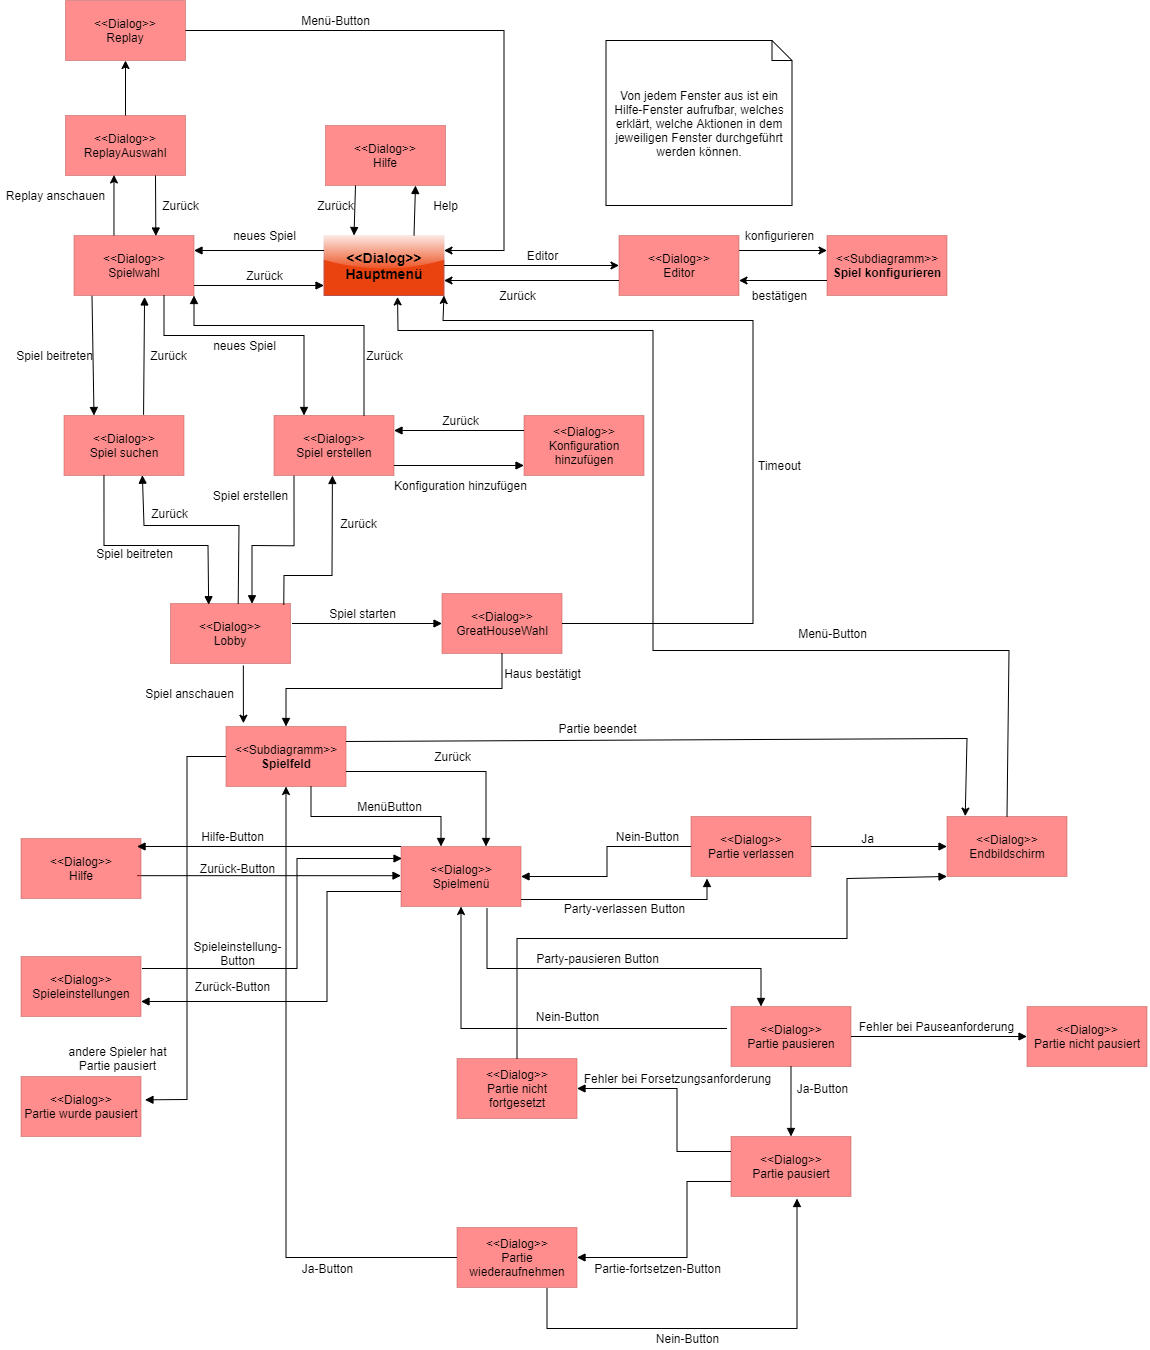
\includegraphics[width=\textwidth]{images/meilen3_a1_Hauptdiagramm}
\captionof{figure}{Dialogstruktur für den grundlegenden Spielstart und -ablauf}


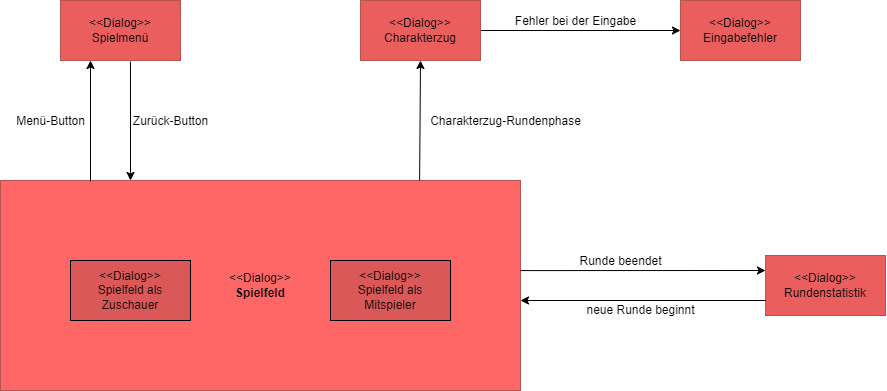
\includegraphics[width=\textwidth]{images/meilen3_a1_Spielfeld}
\captionof{figure}{Dialogstruktur für das Spielfeld und die Optionen während des Spiels. Generell gibt es einen Dialog für das Spielfeld, welcher jedoch je nach Benutzer anders aussieht. Wenn das Spielfeld für einen Zuschauer aufgerufen wird, dann sieht das Spielfeld anders aus, als bei einem Spieler. Deswegen gibt es spezialisierte Dialoge für das \glqq{}Spielfeld\grqq{}}


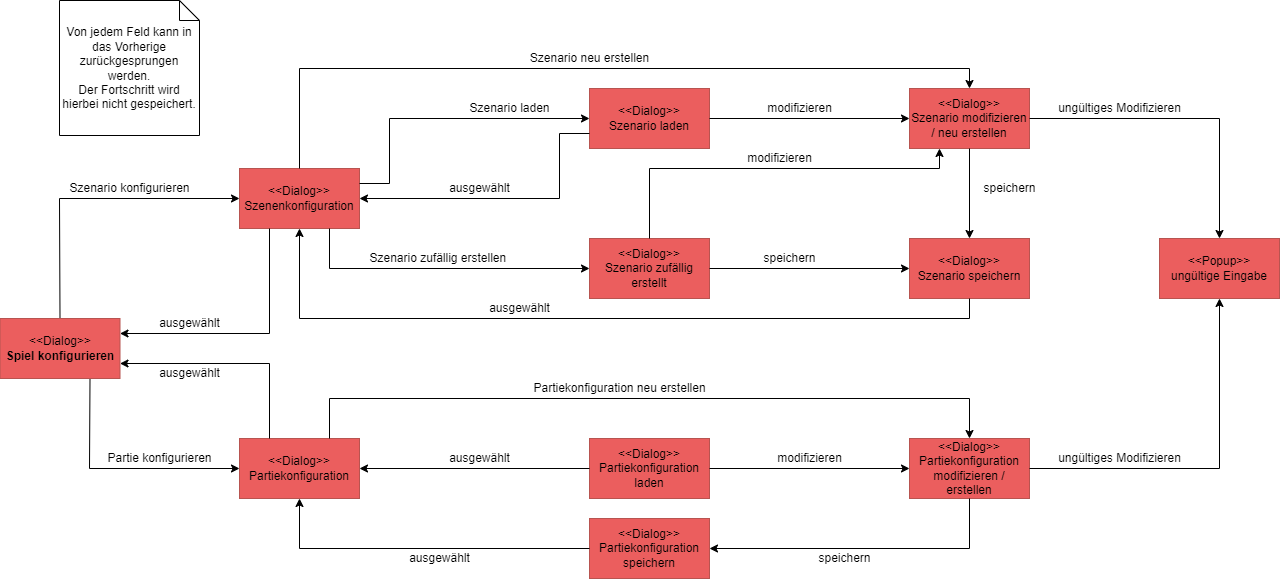
\includegraphics[width=\textwidth]{images/meilen3_a1_Spielkonfiguration}
\captionof{figure}{Dialogstruktur für die Spielkonfiguration}

Das für das Spiel zu viele Dialoge existieren wurden die Dialoge bzw. das Dialogstrukturdiagramm der Übersichtlichkeit halber aufgeteilt. In das jeweilige Subdiagramm kommt man, wenn man einen Dialog erreicht, der mit \textit{<<Subdiagramm>>} gekennzeichnet ist. \\ Dabei gibt es folgende Zuordnung der Dialoge und Anwendungsfällen aus \autoref{sssec:use-cases}, wobei in dem Kapitel auch die entsprechenden Anforderungen zugeordnet sind: 

\vspace{0.5cm}

\begin{tabularx}{\linewidth}{p{4cm}|p{7cm}|l}
	\textbf{Dialog} & \textbf{zugeordneter Anwendungsfall} & Typ \\
	\hline
	Replay & Replay abspielen & Dialog \\
	Replay/Auswahl & Replay abspielen & Dialog \\
	Hilfe & kein konkreter Anwendungsfall; siehe \nfaref{QA-Bedienbarkeit} \\			Spielwahl & Teilnahme als Zuschauer / Mitspieler & Dialog \\
	Hauptmenü & Teilnahme als Zuschauer / Mitspieler & Dialog \\
	Editor & Spiel konfigurieren und laden & Dialog \\
	Spiel suchen & Teilnahme als Zuschauer / Mitspieler & Dialog \\
	Spiel erstellen & Teilnahme als Zuschauer / Mitspieler & Dialog \\
	Konfiguration hinzufügen & Spiel konfigurieren und laden & Dialog \\
	Lobby & Teilnahme als Zuschauer / Mitspieler & Dialog \\
	Great House Wahl & Great House Wahl & Dialog \\
	Spielmenü & Partie pausieren und fortsetzen & Dialog \\
	Partie wurde pausiert & Partie pausieren und fortsetzen & Hinweisfenster \\
	Partie verlassen & Partie beenden & Bestätigungsfenster \\
	Endbildschirm & Partie beenden & Hinweisfenster \\ 	
	Partie pausieren & Partie pausieren und fortsetzen & Bestätigungsfenster \\
	Partie nicht pausiert & Partie pausieren und fortsetzen & Fehlerbenachrichtigung \\		
	Partie pausiert & Partie pausieren und fortsetzen & Hinweisfenster \\	
	Partie nicht fortgesetzt & Partie pausieren und fortsetzen & Fehlerbenachrichtigung \\ 
	Partie wiederaufnehmen & Partie pausieren und fortsetzen & Bestätigungsfenster \\
	Spielfeld & Spielfeld und -zustand anzeigen & Dialog \\
	Charakterzug & Charakterzug (Bewegung und Aktion von Charakter) & Dialog \\ 
	Eingabefehler & Charakterzug (Bewegung und Aktion von Charakter) & Fehlerbenachrichtigung \\
	Rundenstatistik & Spielfeld und -zustand anzeigen & Hinweisfenster \\ 
	Spiel konfigurieren & Spiel konfigurieren und laden & Dialog \\ 
	Szenariokonfiguration & Szenario erstellen und konfigurieren & Dialog \\ 
	Szenario laden & Szenario erstellen und konfigurieren & Dialog \\
	Szenario modifizieren / neu erstellen & Szenario erstellen und konfigurieren & Dialog \\
	Szenario zufällig erstellt & Szenario erstellen und konfigurieren & Dialog \\
	Szenario speichern & Szenario erstellen und konfigurieren & Bestätigungsfenster \\
	ungültige Eingabe & Spiel konfigurieren und laden & Fehlerbenachrichtigung \\
	Partiekonfigurarion laden & Partie konfigurieren & Dialog \\
	Partiekonfigurarion modifizieren / neu erstellen & Partie konfigurieren & Dialog \\
	Partiekonfigurarion speichern & Partie konfigurieren & Bestätigungsfenster \\
	Partiekonfiguration & Partie konfigurieren & Dialog 
\end{tabularx}

\subsubsection{Graphische Gestaltung und Nutzungskonzept}
Im Folgenden sind die verschiedenen graphische Prototypen in Form von \glqq{}Mockup\grqq{}-Zeichnung aufgelistet. Für jeden graphischen Prototypen wird in textuellen Form zusätzlich beschrieben, was die Elemente auf der Oberfläche bedeuten und wie dieser Dialog bedient werden kann. 

\begin{center}
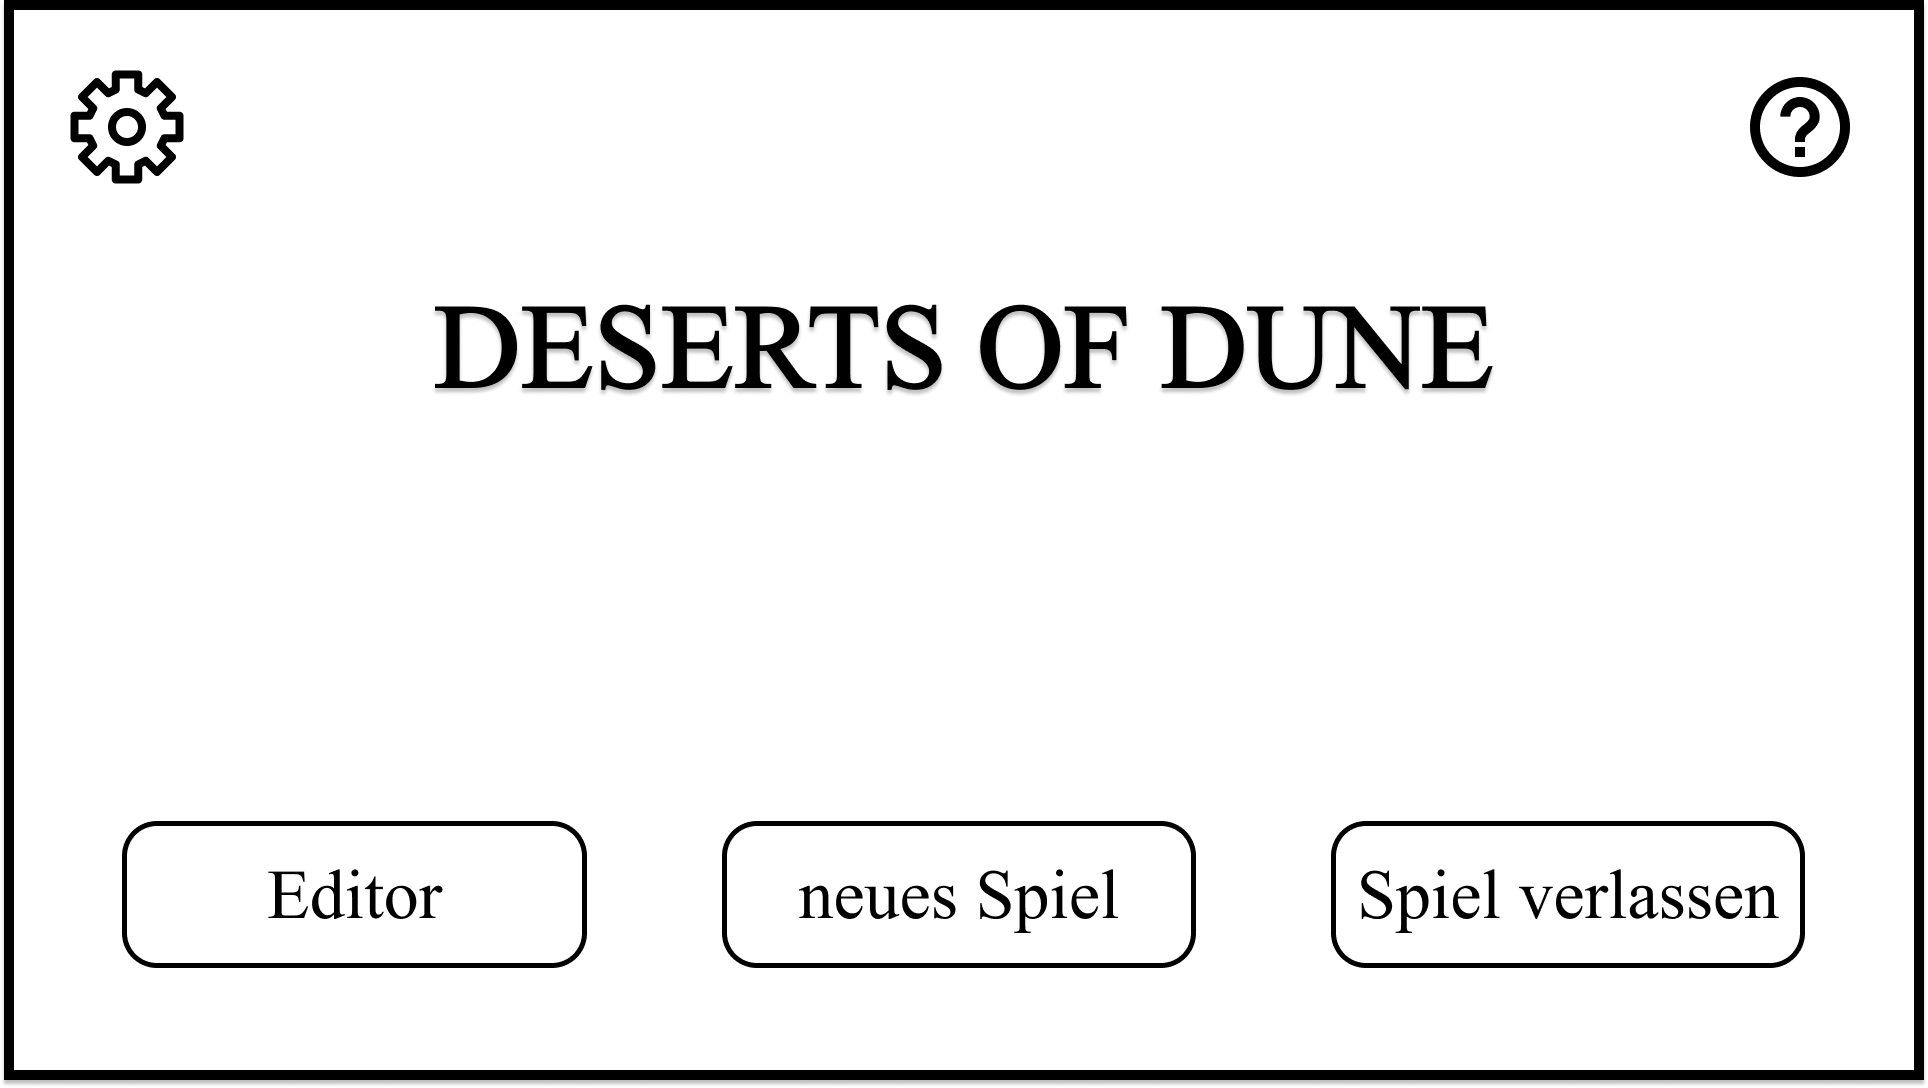
\includegraphics[width=\textwidth]{images/Hauptmenue}
\captionof{figure}{\textbf{Hauptmenü}:\\
Der \glqq Hauptmenü\grqq -Dialog wird beim Starten der Anwendung zu Beginn angezeigt. In diesem Dialog hat der Benutzer die Möglichkeit den Editor zu starten, ein neues Spiel zu starten oder die Anwendung wieder zu schließen, indem er die entsprechenden Buttons drückt.}

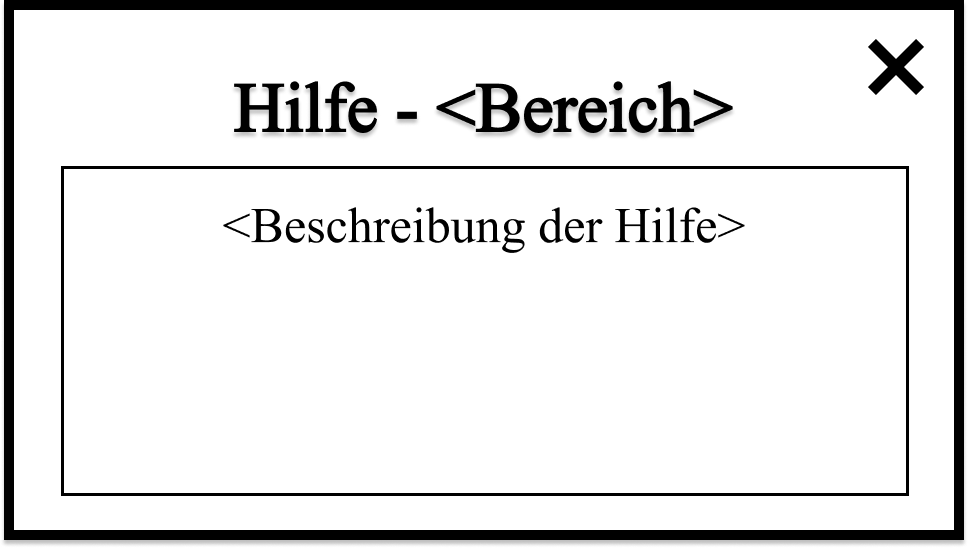
\includegraphics[width=0.7\textwidth]{images/Hilfe}
\captionof{figure}{\textbf{Hilfe}:\\
Der \glqq Hilfe\grqq -Dialog kann von jedem Dialog, bei dem das Fragezeichen rechts oben im Eck, aufgerufen werden und hier wird zu dem Dialog, wovon es aufgerufen wurde, eine kurze Beschreibung zu dem jeweiligen Dialog stehen}

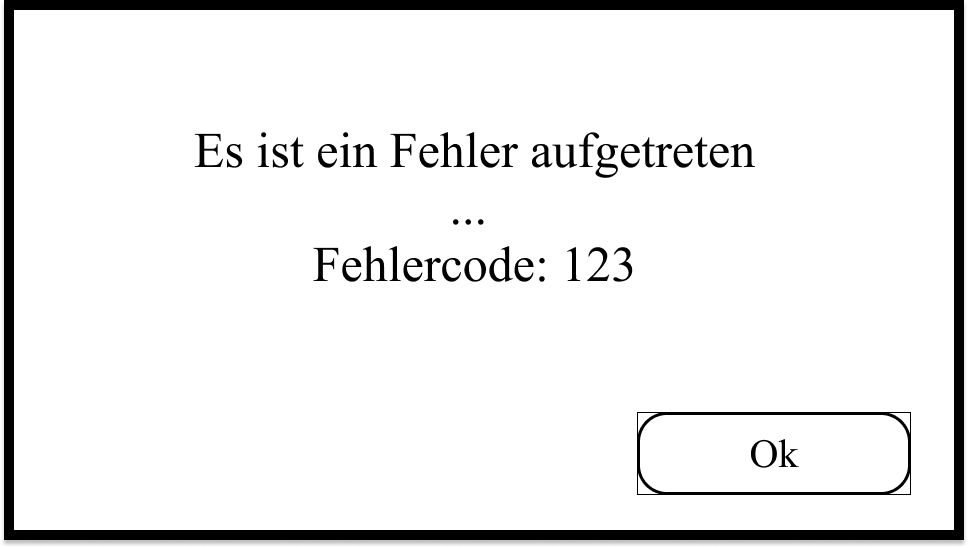
\includegraphics[width=0.7\textwidth]{images/Fehlerbenachrichtigung}
\captionof{figure}{\textbf{allgemeine Fehlerbenachrichtigung (analog Hinweisfenster)}:\\
Der \glqq{}Fehlerbenachrichtung\grqq{}-Dialog taucht immer dann auf, wenn es zu einem Fehler kam. Dieser Dialog zeigt dem Benutzer einen Text an und der Dialog lässt sich schließen, wenn der Benutzer den \textit{OK}-Button betätigt. Damit bestätigt er, dass er den Text gelesen hat oder das Fenster nicht mehr sehen will. \\ Der Dialog für ein Hinweisfenster sieht identisch aus, nur das ein anderer Text angezeigt wird. 
}

\includegraphics[width=0.7\textwidth]{images/Bestätigungsfenster}
\captionof{figure}{\textbf{Bestätigungsfenster}:\\
Der Dialog \glqq{}Bestätigungsfenster\grqq{} wird immer dann dem Benutzer angezeigt, wenn eine wichtige Aktion des Benutzers bestätigt werden soll, zum Beispiel wenn der Benutzer das Spiel verlassen will. Dann hat der Nutzer, die Aktion mit \textit{Ok} zu bestätigen oder mit \textit{Abbrechen} zu dem Dialog zurückkehren, von dem er gekommen ist.
}

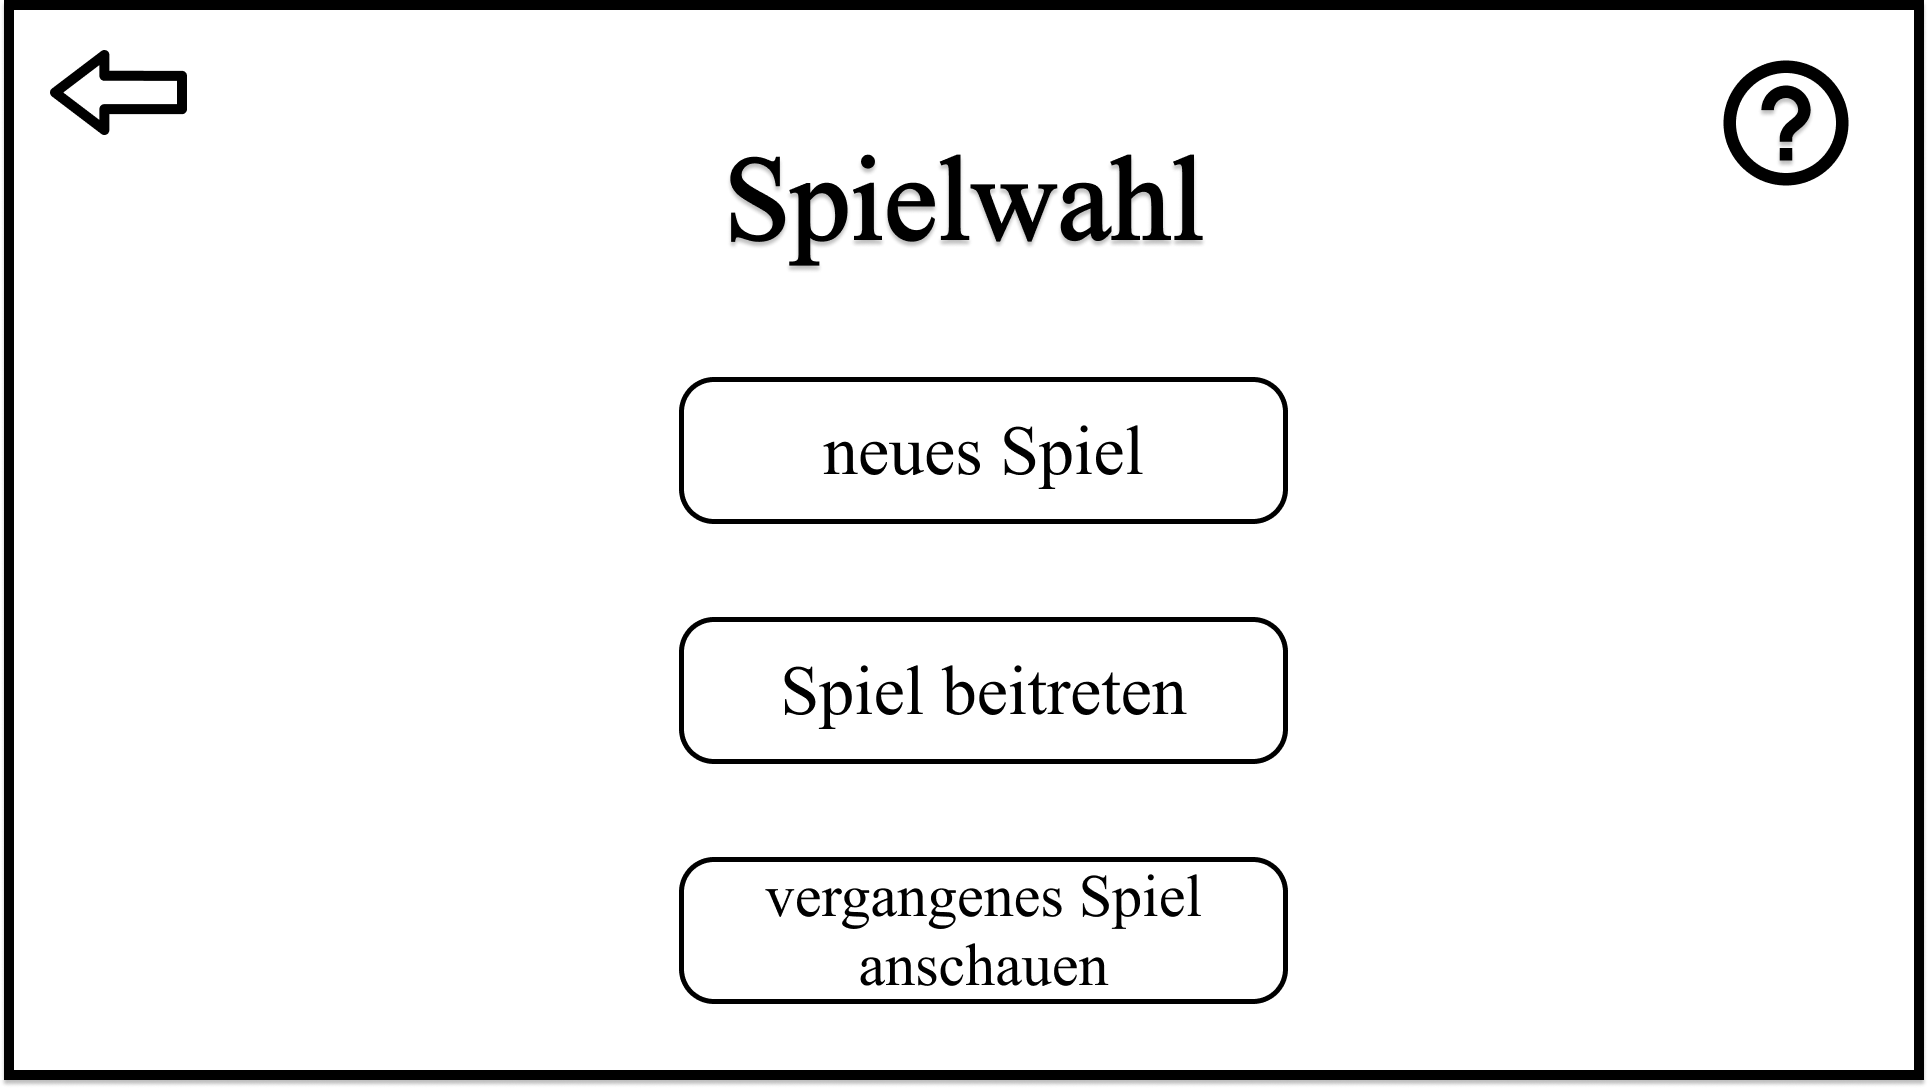
\includegraphics[width=\textwidth]{images/Spielwahl}
\captionof{figure}{\textbf{Spielwahl}: Hier kann der Nutzer auswählen, ob er einem bereits erstellten Spiel beitreten will, selbst ein Spiel erstellen möchte oder ein vergangenes Spiel nochmals anschauen will.}

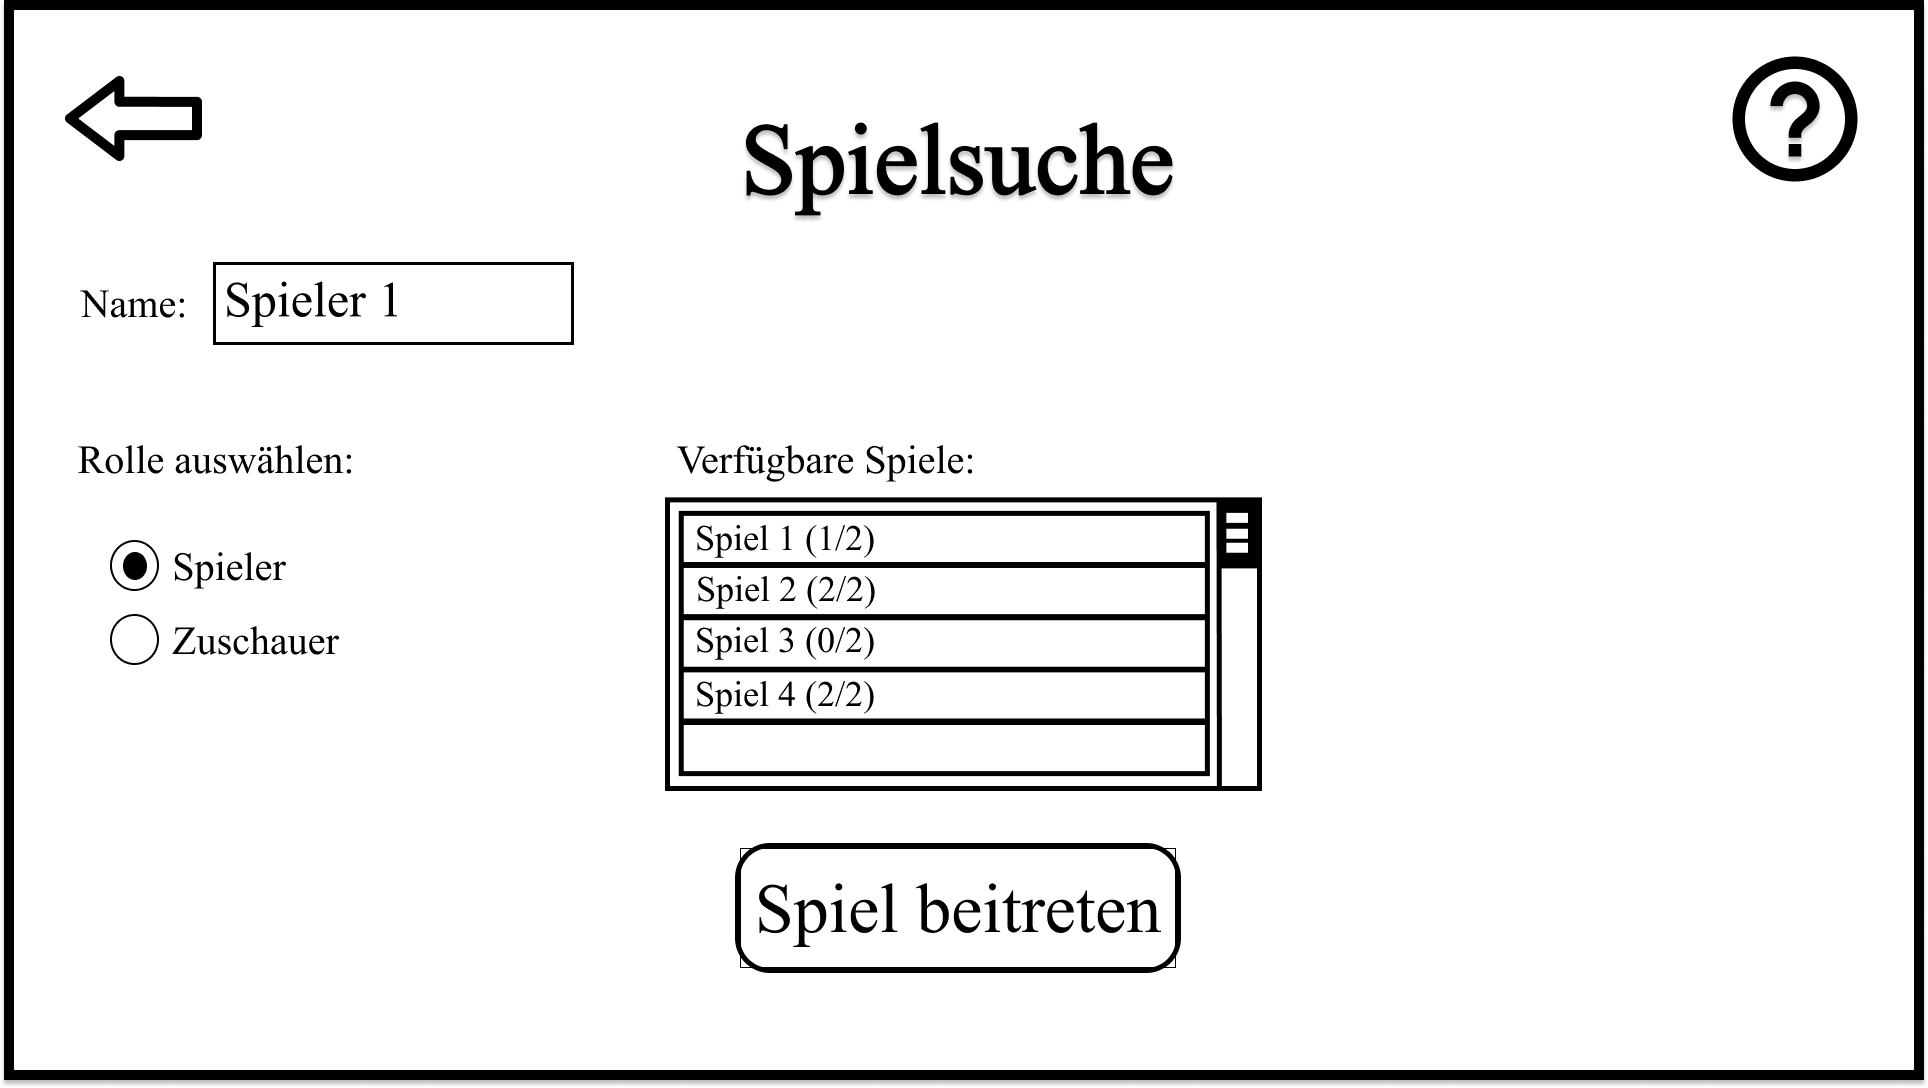
\includegraphics[width=\textwidth]{images/Spielsuche}
\captionof{figure}{\textbf{Spiel suchen}:\\
Wurde im Spielwahl-Dialog der \glqq Spiel beitreten\grqq -Button gedrückt, kann der Nutzer jetzt einem bereits erstellten Spiel beitreten. \\
Hier kann der Nutzer seinen Namen eingeben und seine Rolle wählen, also ob er als Spieler oder als Zuschauer beitreten möchte. Dem Nutzer werden alle verfügbaren Spiele angezeigt und wenn in einem Spiel schon zwei Spieler sind, kann man dort nur noch als Zuschauer beitreten. Durch drücken auf den \glqq Spiel beitreten\grqq -Button kommt der Nutzer in den \glqq Lobby\grqq -Dialog.}

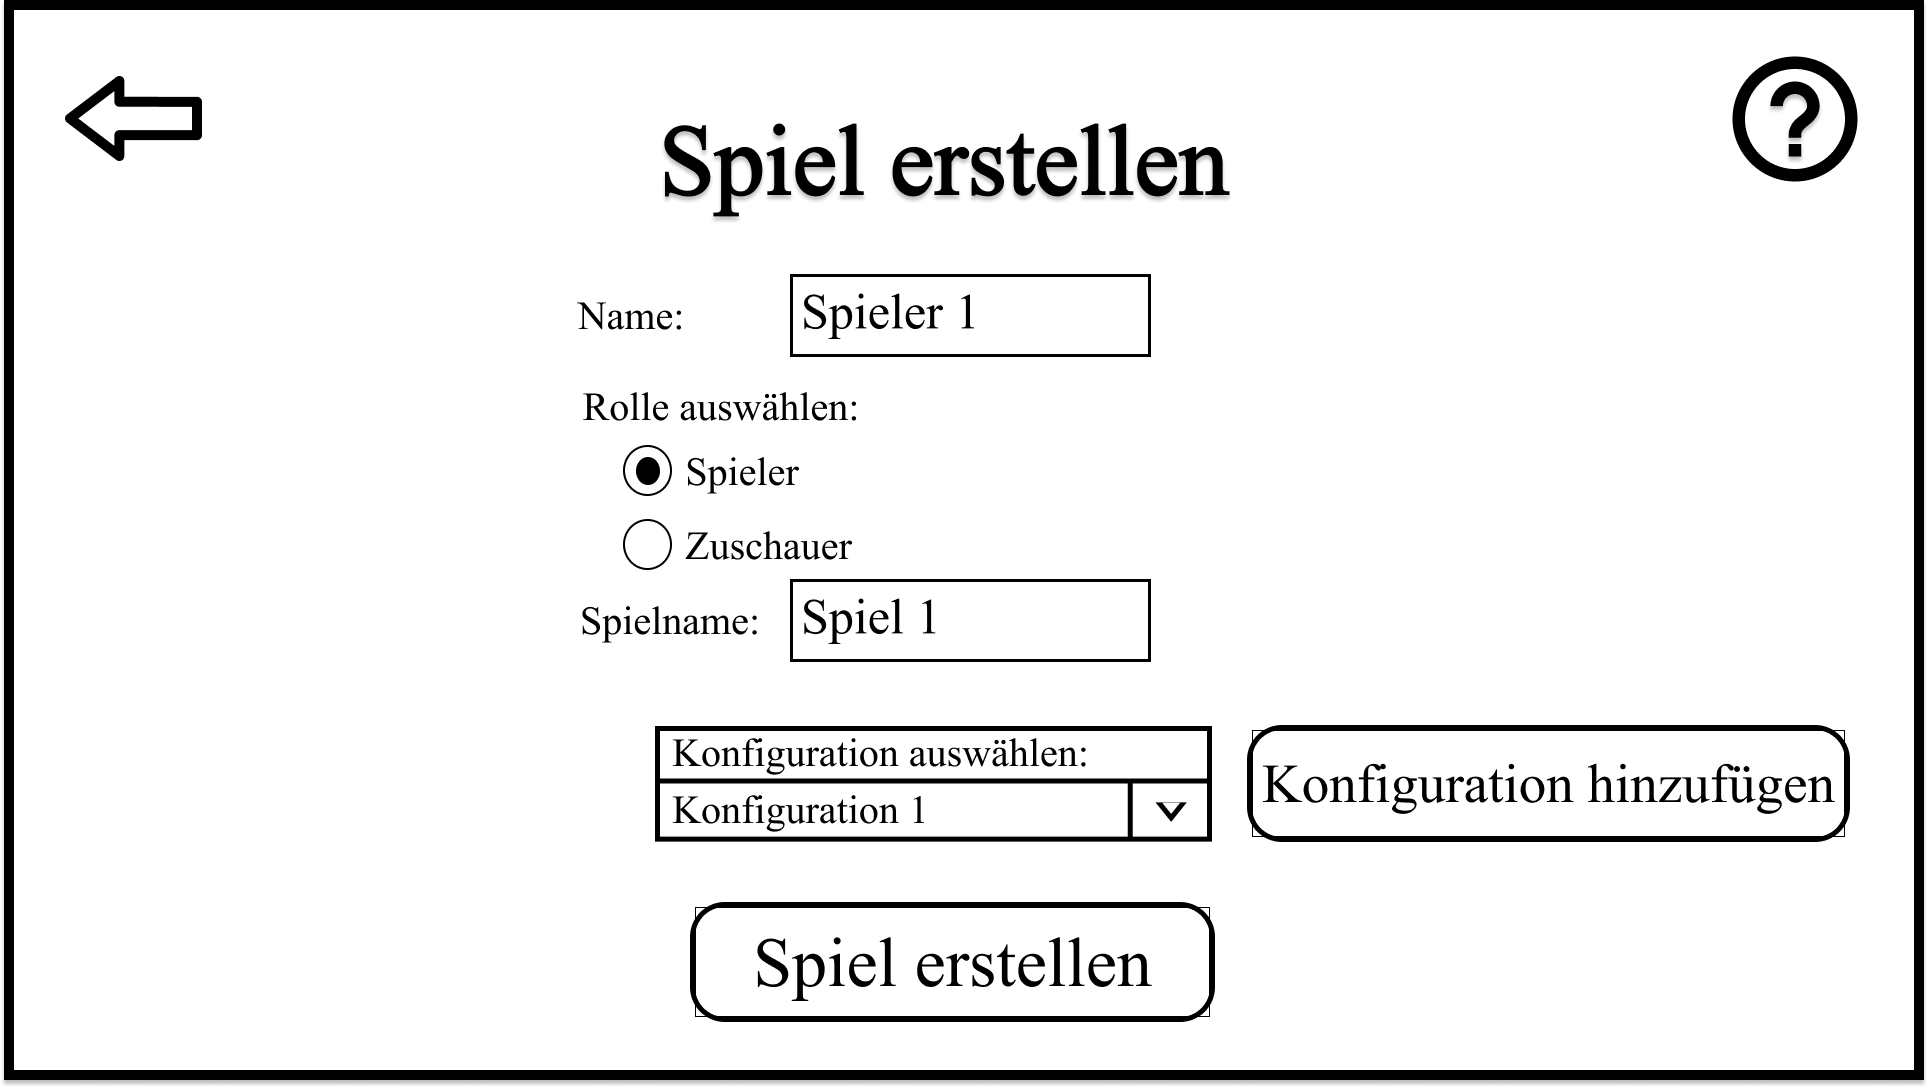
\includegraphics[width=\textwidth]{images/Spiel_erstellen}
\captionof{figure}{\textbf{Spiel erstellen}: \\
Wurde im Spielwahl-Dialog der \glqq Neues Spiel\grqq -Button gedrückt, kann der Nutzer jetzt ein neues Spiel erstellen.\\
Er kann dabei seinen Namen eingeben und den Namen des Spiels. Außerdem kann er auch hier seine Rolle auswählen, ob er Spieler oder Zuschauer sein möchte. Er hat zusätzlich ein Dropdown-Menü, bei dem er eine bereits hinzugefügte Konfiguration auswählen kann oder er kann auch selbst eine neue Spielkonfiguration hinzufügen mit dem \glqq Konfiguration hinzufügen\grqq -Button.}

\includegraphics[width=\textwidth]{images/Konfiguration_hinzufügen}
\captionof{figure}{\textbf{Konfiguration hinzufügen}:\\
Wurde im \glqq Spiel erstellen\grqq -Dialog der \glqq Konfiguration hinzufügen\grqq -Button gedrückt, kommt man in diesen Dialog, bei dem man in einer Textbox den Pfad und den Dateinamen für eine erstellte Konfiguration eingeben kann und dieses dann hinzugefügt wird.\\}

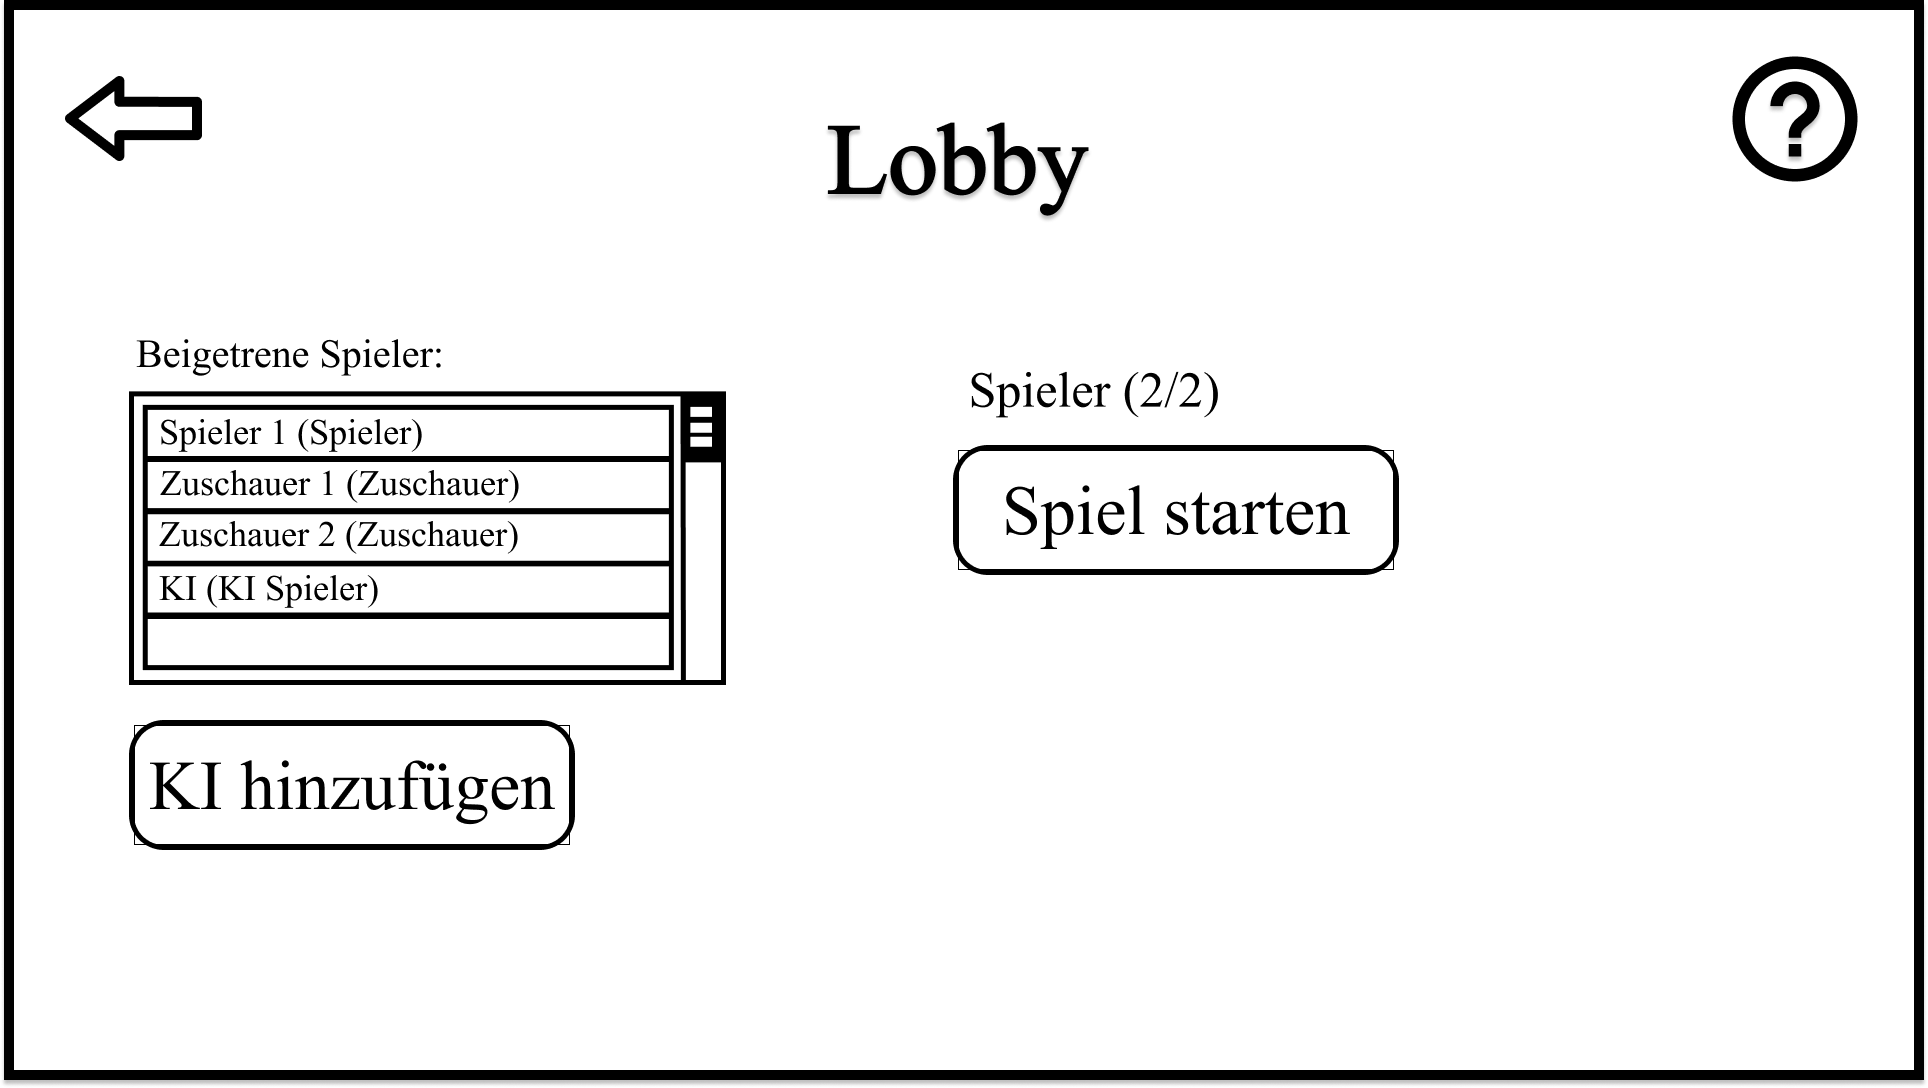
\includegraphics[width=\textwidth]{images/Lobby}
\captionof{figure}{\textbf{Lobby}:\\
In dem \glqq Lobby\grqq -Dialog werden in einer Liste alle bereits beigetretenen Spieler und Zuschauer angezeigt. Hier besteht auch die Option einen KI-Spieler über einen Button hinzuzufügen. Außerdem ist hier noch ein \glqq Spiel starten\grqq -Button, womit man das Spiel starten kann unter der Bedingung, dass zwei Spieler in der Lobby sind.}

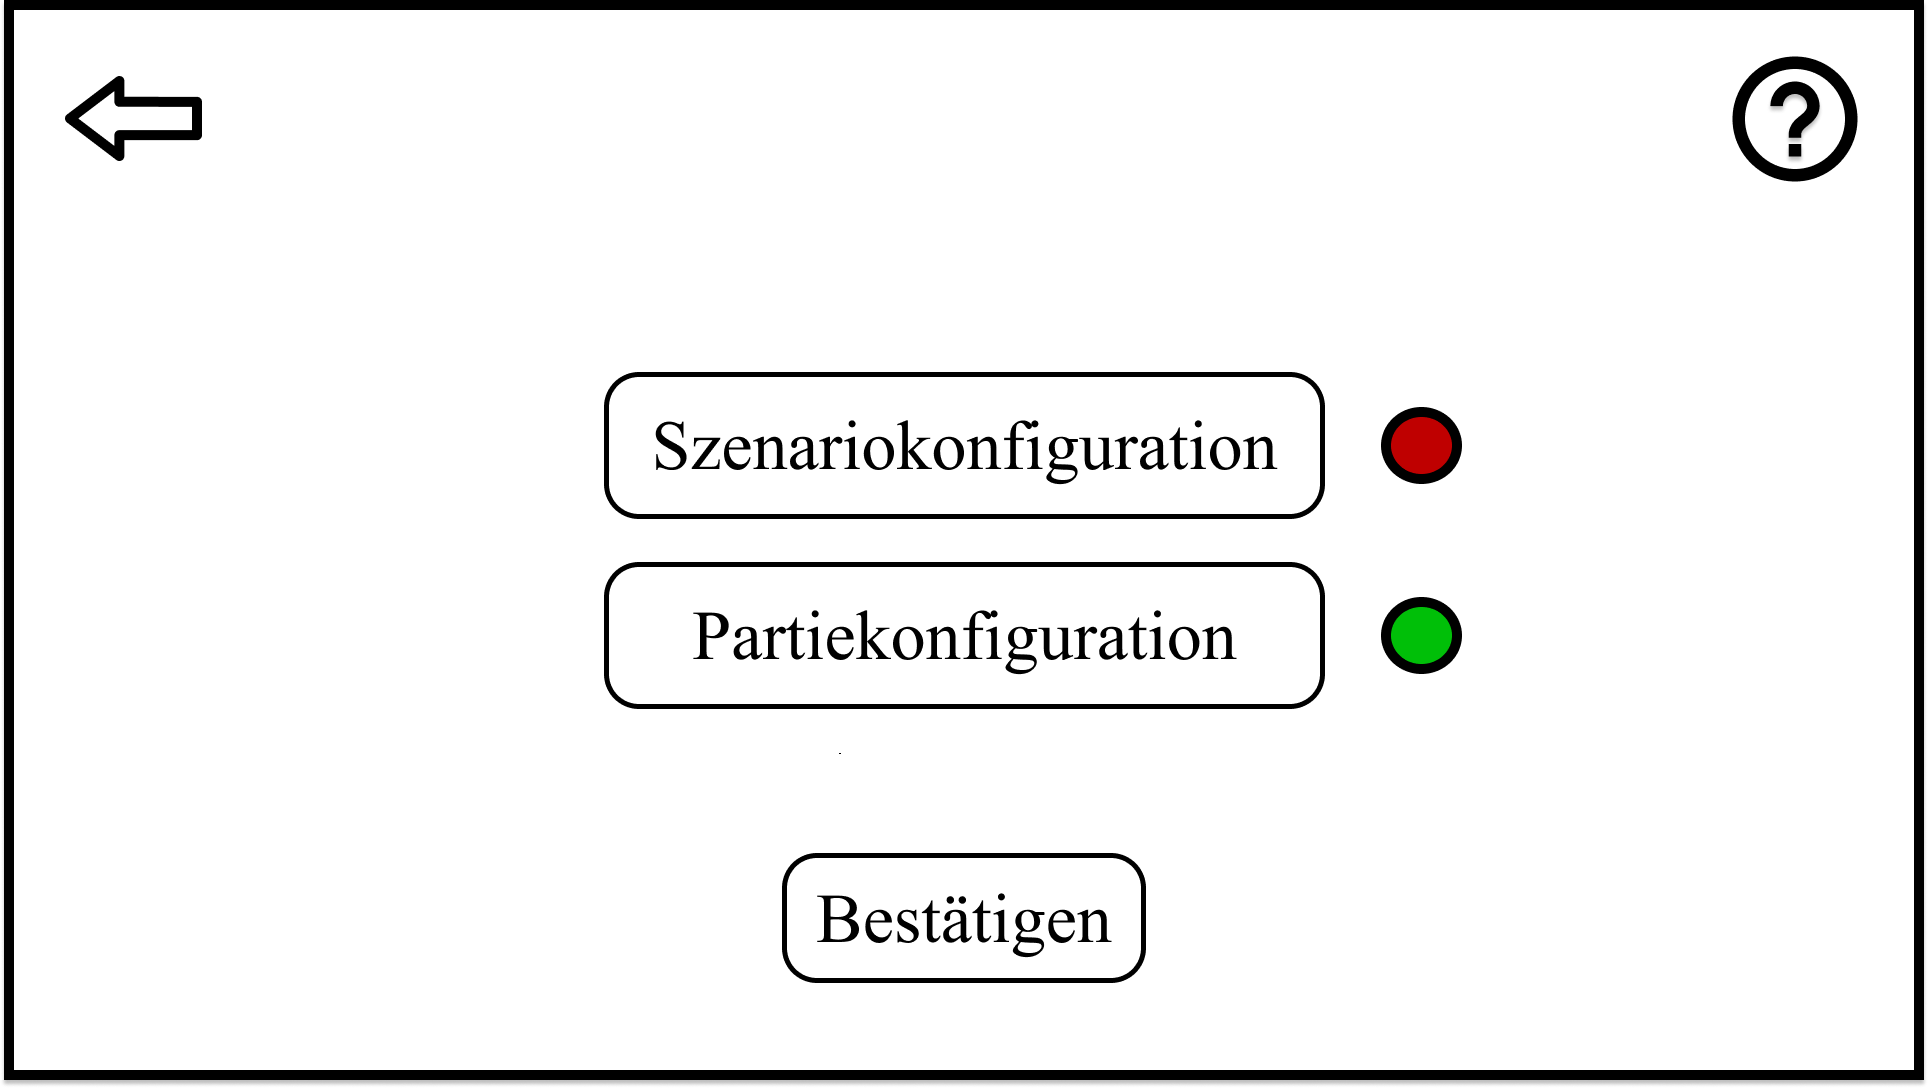
\includegraphics[width=\textwidth]{images/SpielKonfigurieren}
\captionof{figure}{\textbf{Spiel-Konfiguration}:\\
Um eine gültige Spielkonfiguration zu erstellen, muss der Benutzer sowohl eine Senario-Konfiguration, als auch eine Partie-Konfiguration auswählen.
}

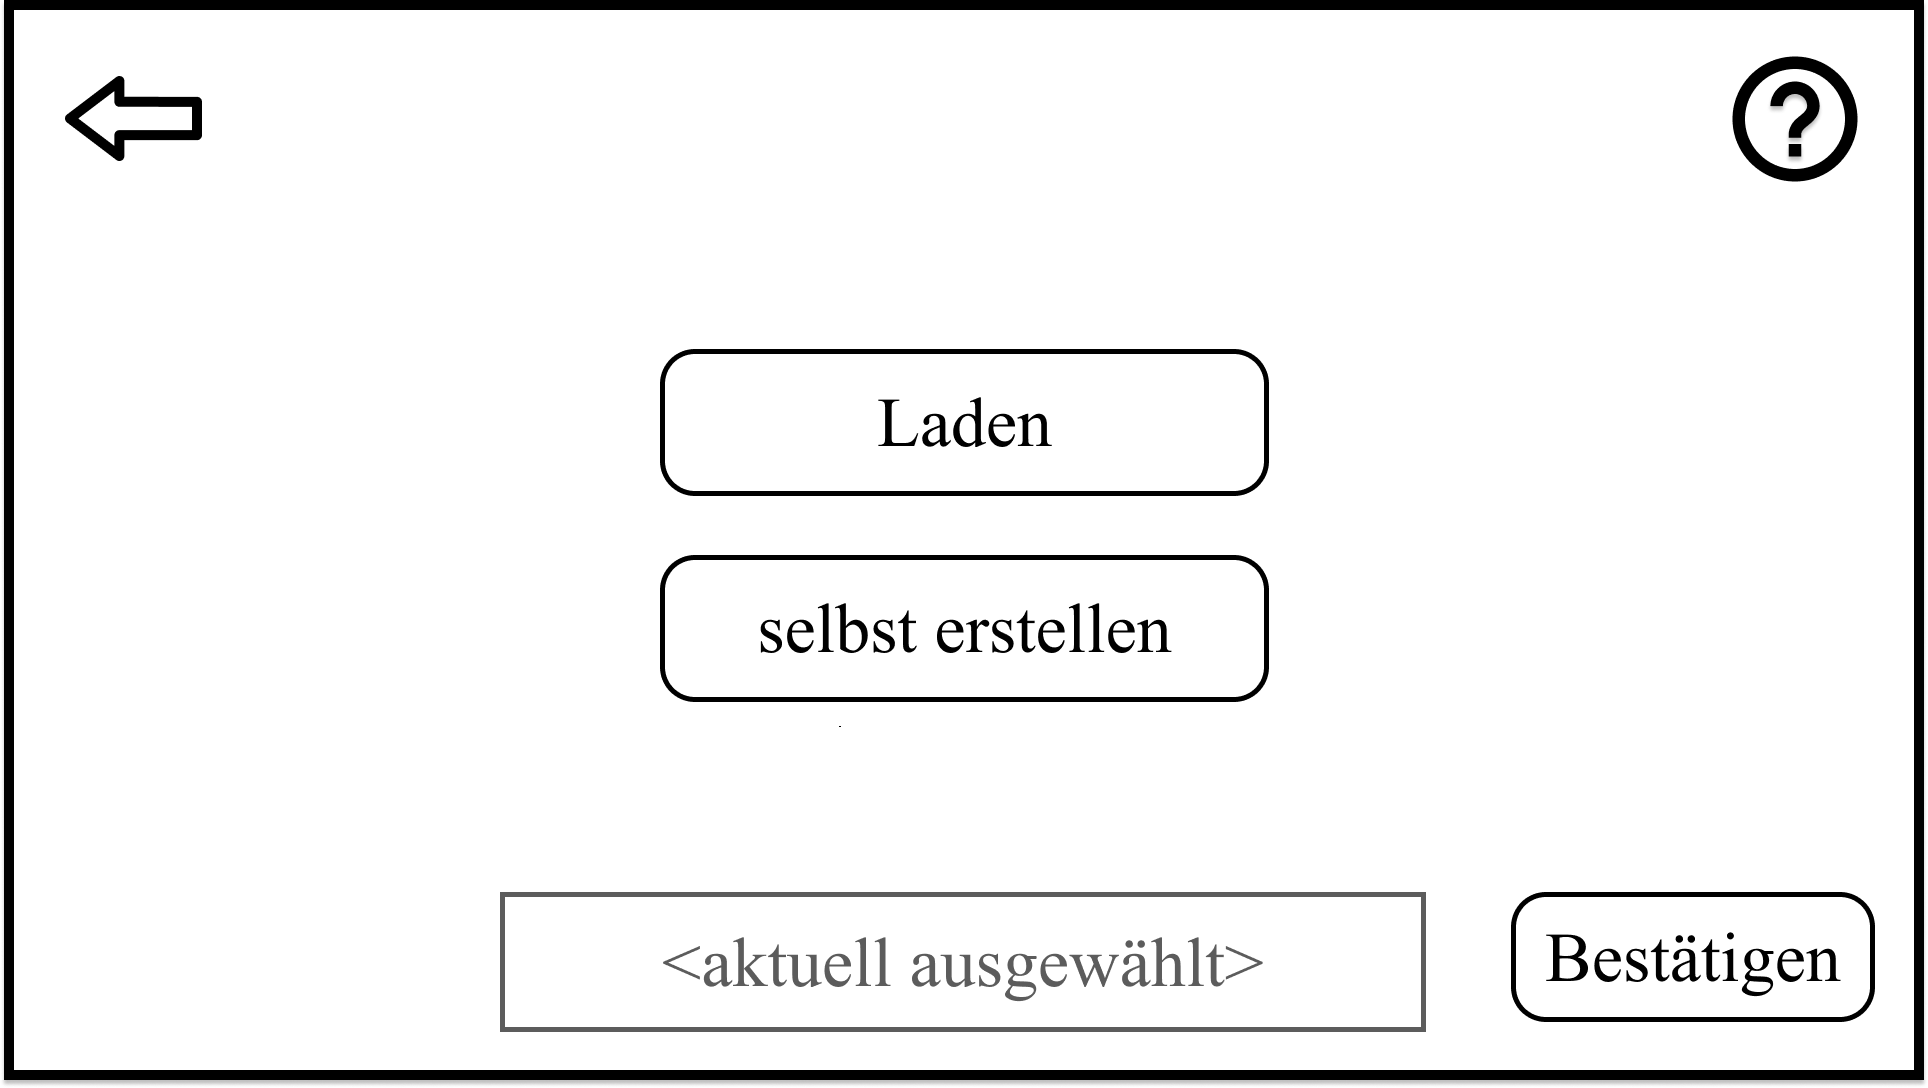
\includegraphics[width=\textwidth]{images/PartieKonfiguration}
\captionof{figure}{\textbf{Partie-Konfiguration}:\\
Der Benutzer kann entweder eine gespeicherte Partie-Konfiguration laden, oder eine neue Partie-Konfiguration erstellen. Der Benutzer kann seine Auswahl bestätigen, aber auch nochmals ändern.
}

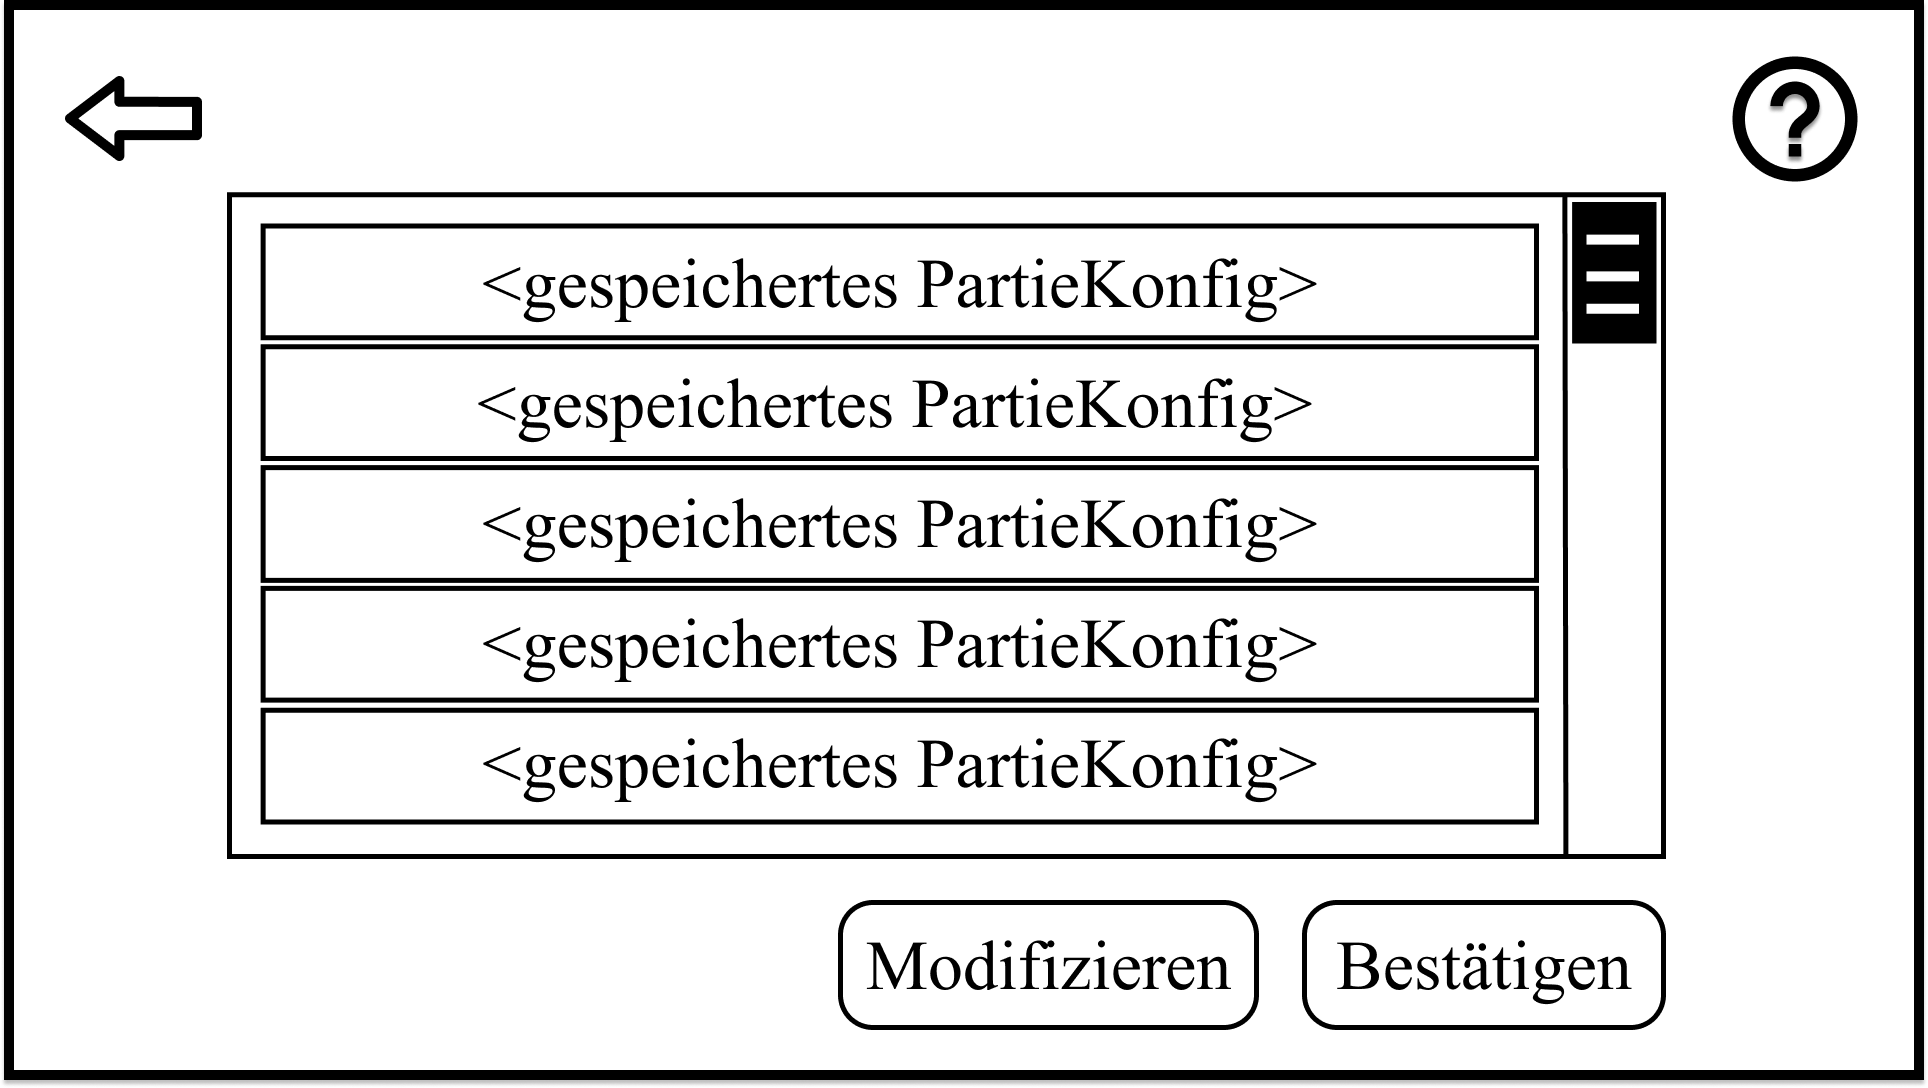
\includegraphics[width=\textwidth]{images/PartiekonfigurationLaden}
\captionof{figure}{\textbf{Partie-Konfiguration laden}:\\
Der Benutzer sieht eine Liste mit gespeicherten Partie-Konfigurationen und kann eine Beliebige auswählen oder modifizieren. 
}

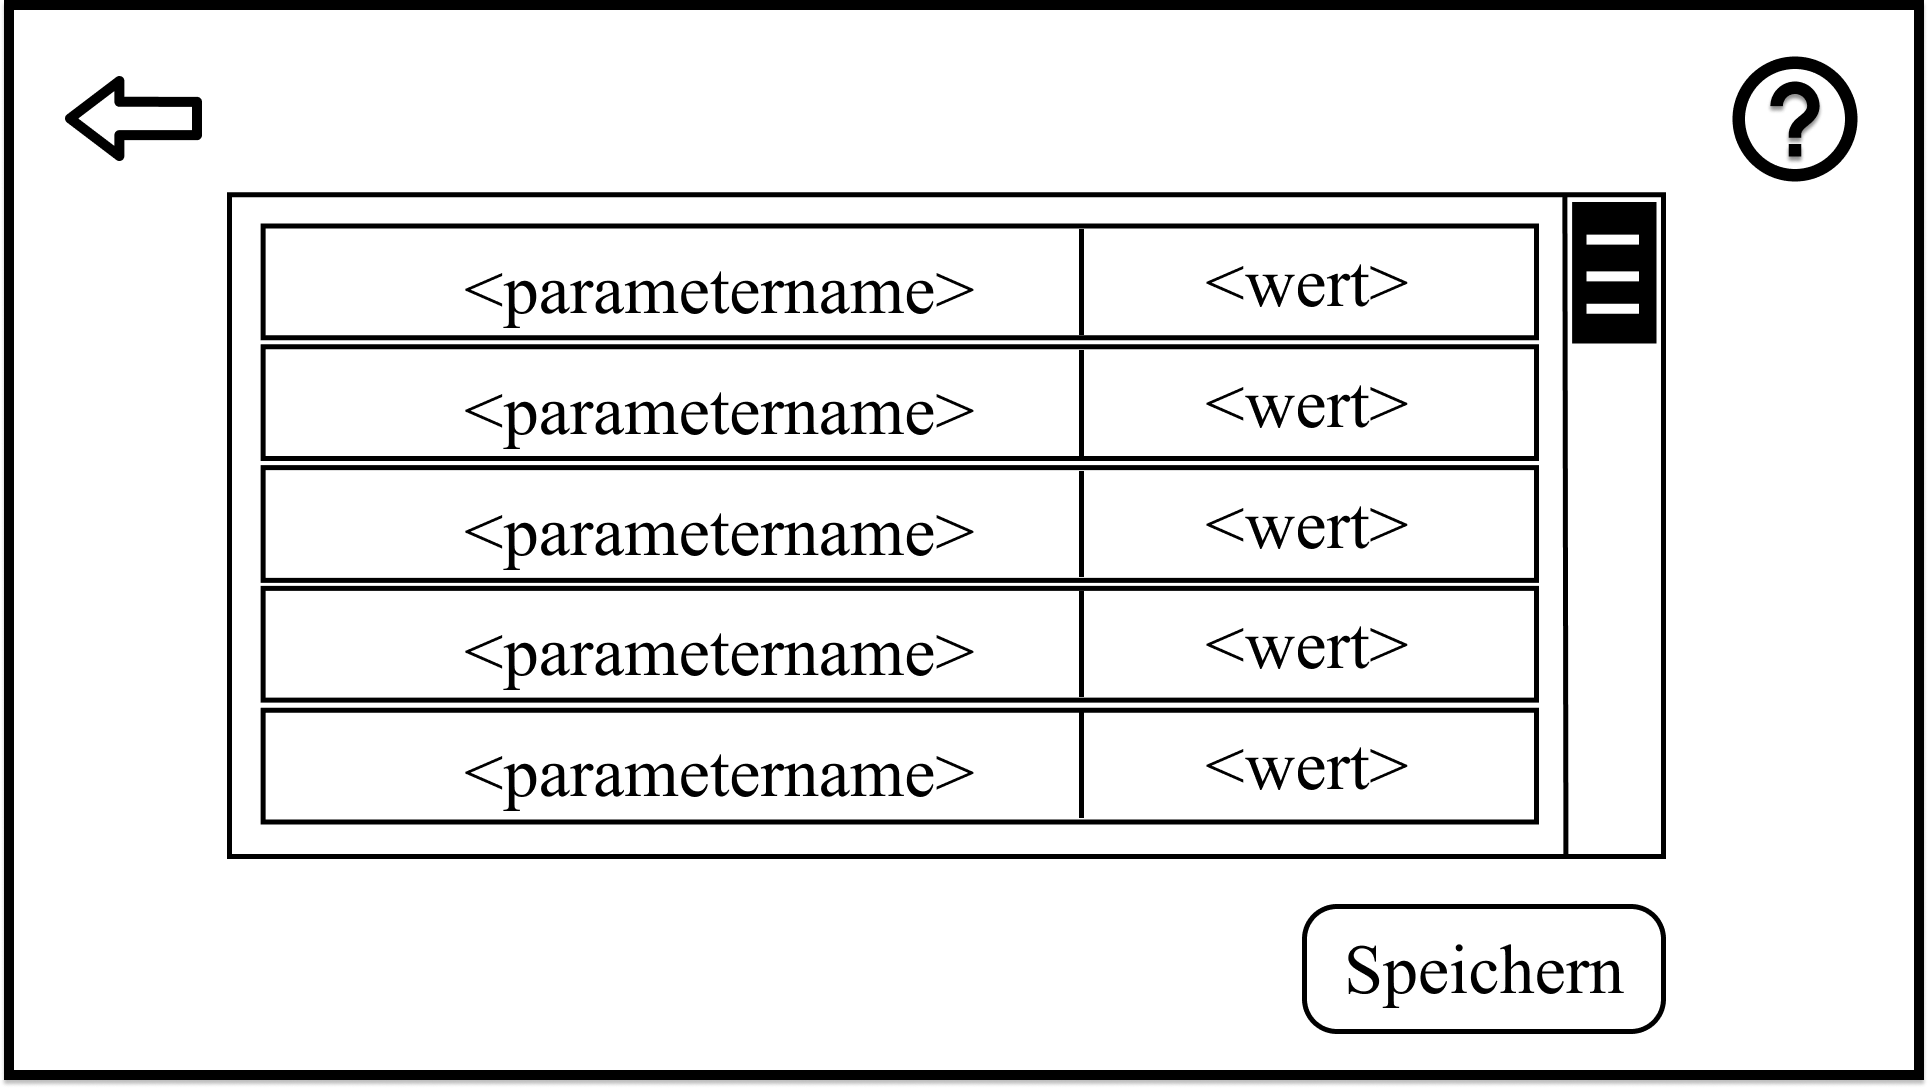
\includegraphics[width=\textwidth]{images/PartieKonfigErstellen}
\captionof{figure}{\textbf{Partie-Konfiguration erstellen / modifizieren}:\\
Der Benutzer legt für jeden Parameter aus der angezeigten Liste einen gewünschten Wert fest. Der Benutzer kann die erstellte/ modifizierte Partie-Konfiguration speichern.
}

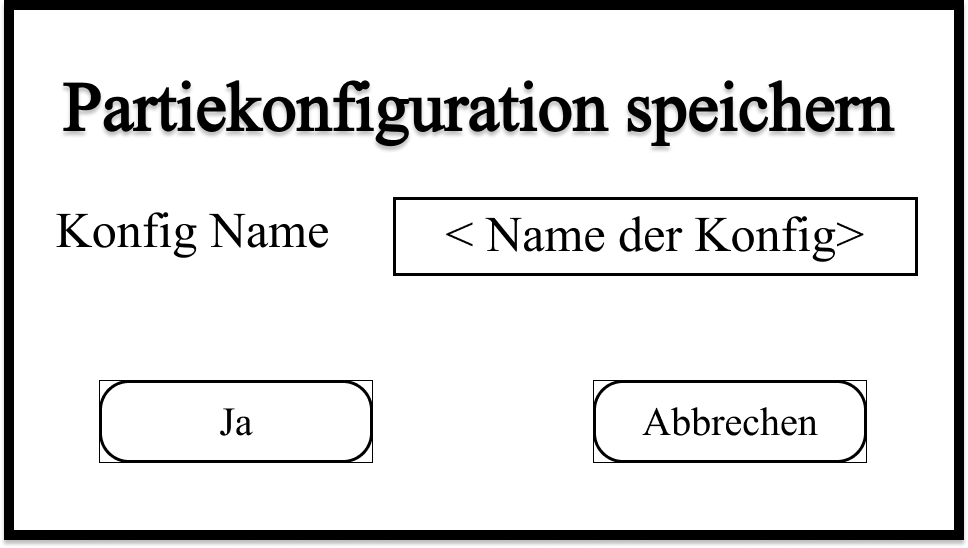
\includegraphics[width=0.7\textwidth]{images/PartiekonfigurationSpeichern}
\captionof{figure}{\textbf{Partie-Konfiguration speichern}:\\
Der Benutzer kann eine soeben erstellte/ modifizierte Partie-Konfiguration speichern, indem er sie benennt und bestätigt. 
}

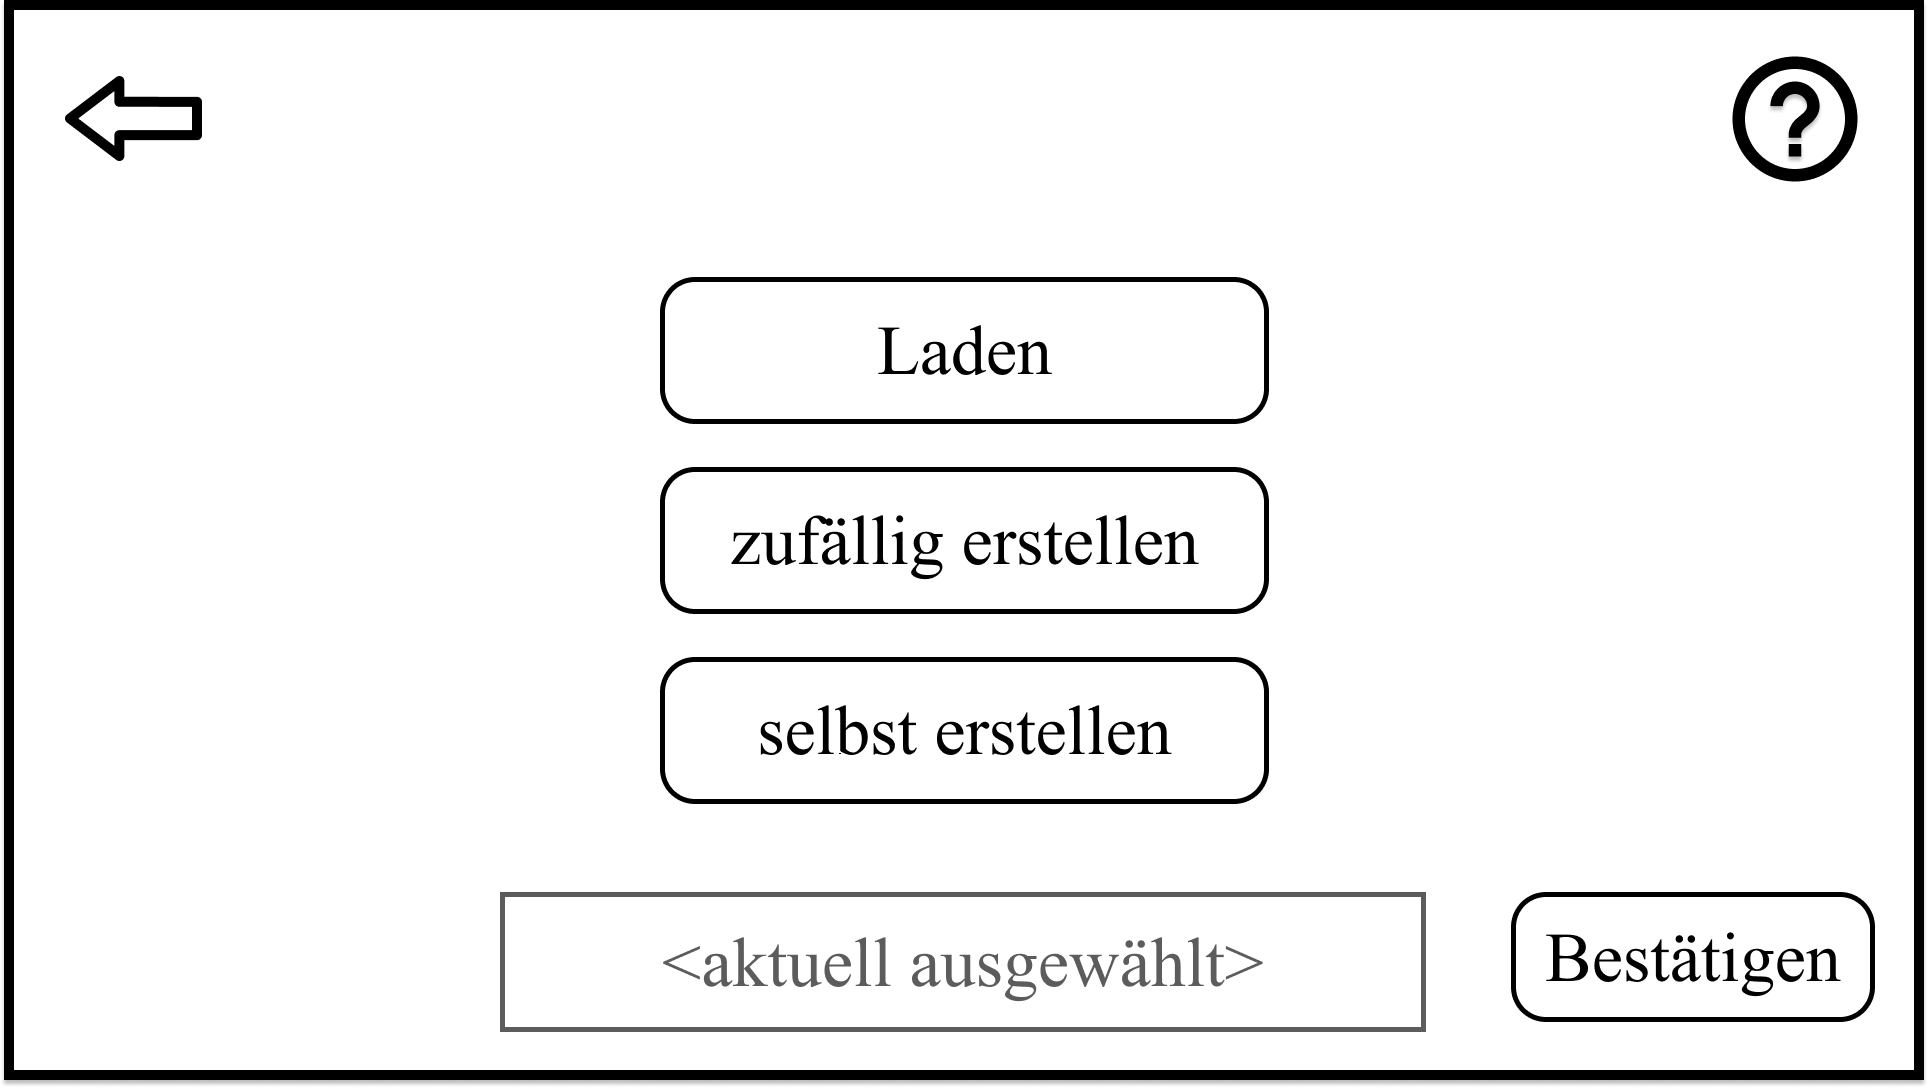
\includegraphics[width=\textwidth]{images/Szenariokonfiguration}
\captionof{figure}{\textbf{Szenario-Konfiguration}:\\
Der Benutzer kann entweder eine gespeicherte Szenario-Konfiguration laden, selbst eine Neue erstellen, oder eine Szenario-Konfiguration zufällig erstellen lassen. Der Benutzer kann seine Auswahl bestätigen, aber auch nochmals ändern.
}

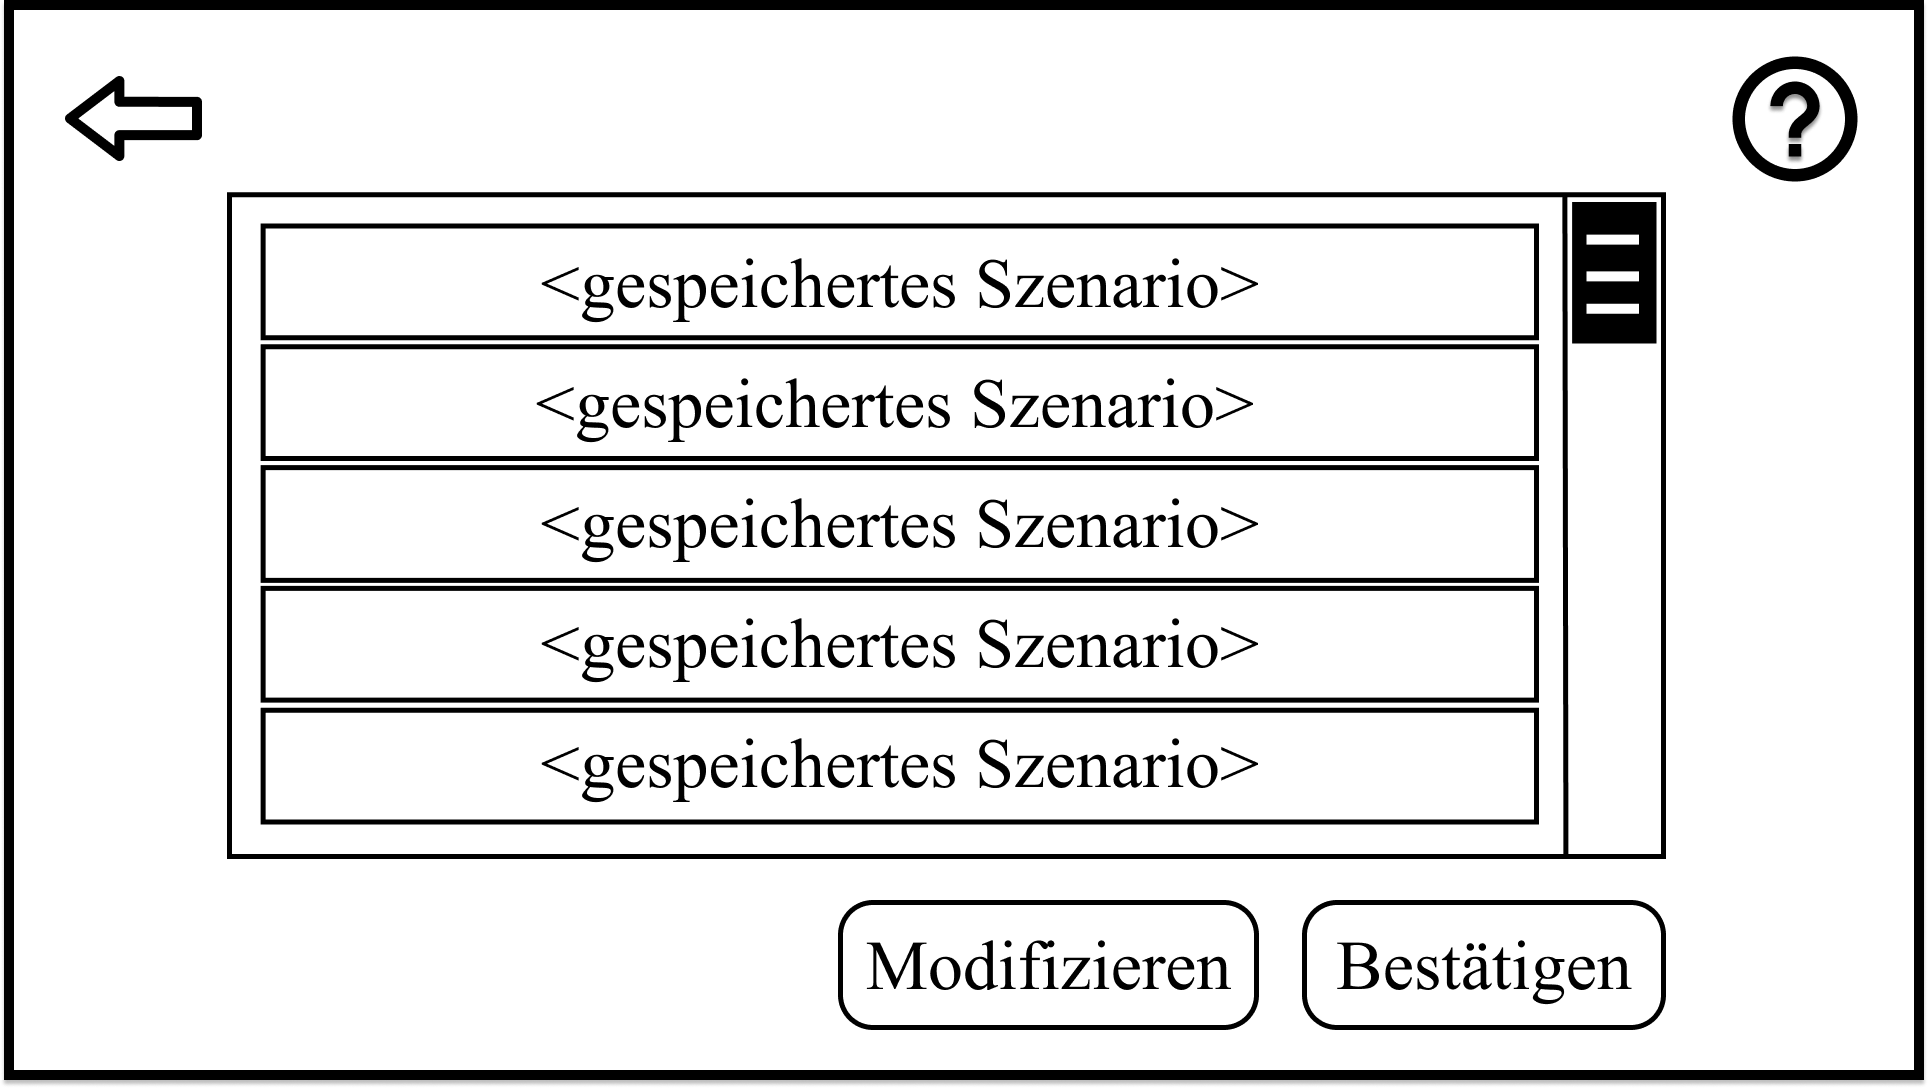
\includegraphics[width=\textwidth]{images/SzenarioLaden}
\captionof{figure}{\textbf{Szenario laden}:\\
Der Benutzer sieht eine Liste mit gespeicherten Szenario-Konfigurationen und kann eine Beliebige auswählen oder modifizieren.
}

\includegraphics[width=\textwidth]{images/SzenarioZufälligErstellen}
\captionof{figure}{\textbf{Szenario zufällig erstellen}:\\
Der Benutzer kann eine Szenario-Konfiguration zufällig erstellen lassen und bekommt diese dann mit ihren zugehörigen Daten angezeigt. Der Benutzer kann die Szenario-Konfiguration direkt speichern oder nochmal selbst modifizieren.
}

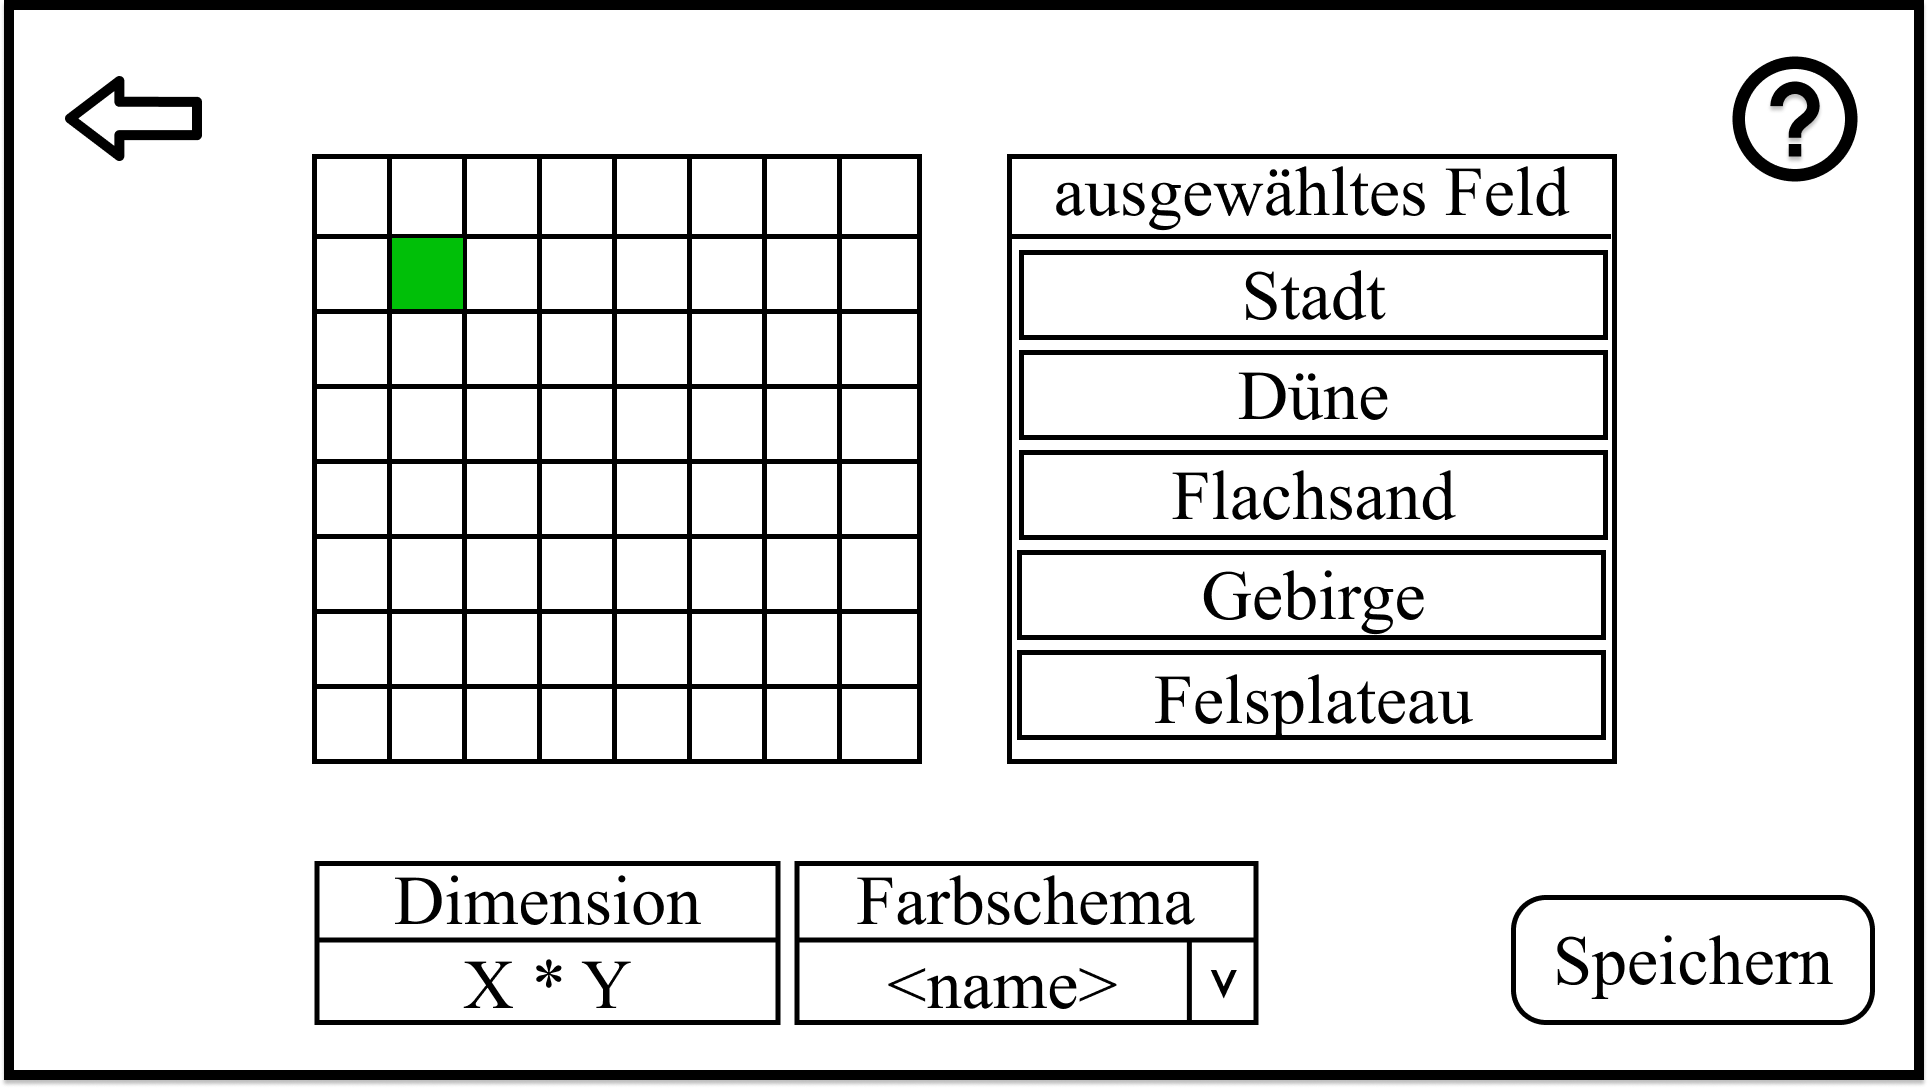
\includegraphics[width=\textwidth]{images/SzenarioErstellen}
\captionof{figure}{\textbf{Szenario erstellen / modifizieren}:\\
Der Benutzer kann verschieden Werte, wie Dimension oder Farbschema festlegen. Der Benutzer kann für die einzelnen Felder die jeweilige Feldart festlegen.
}

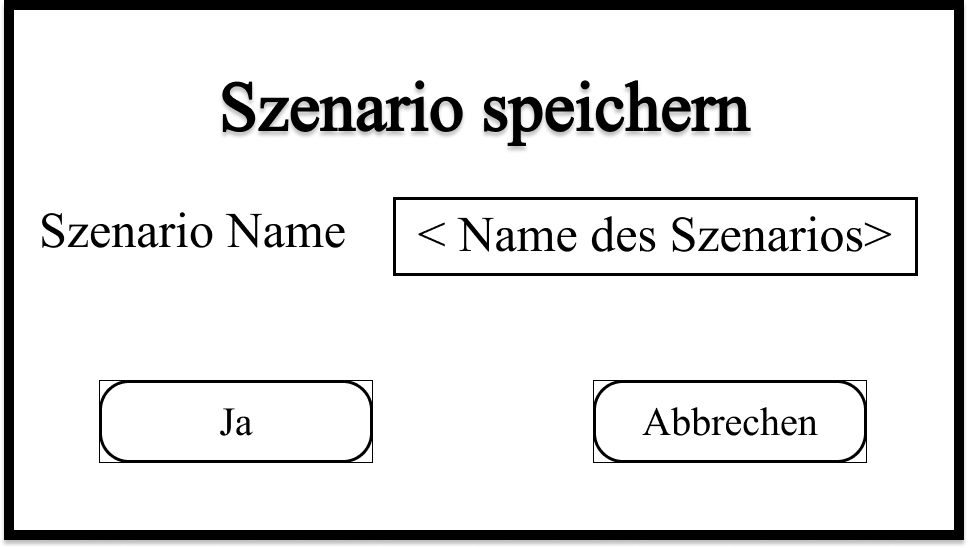
\includegraphics[width=0.7\textwidth]{images/SzenarioSpeichern}
\captionof{figure}{\textbf{Szenario speichern}:\\
Der Benutzer kann eine soeben erstellte/ modifizierte Szenario-Konfiguration speichern, indem er sie benennt und bestätigt.
}

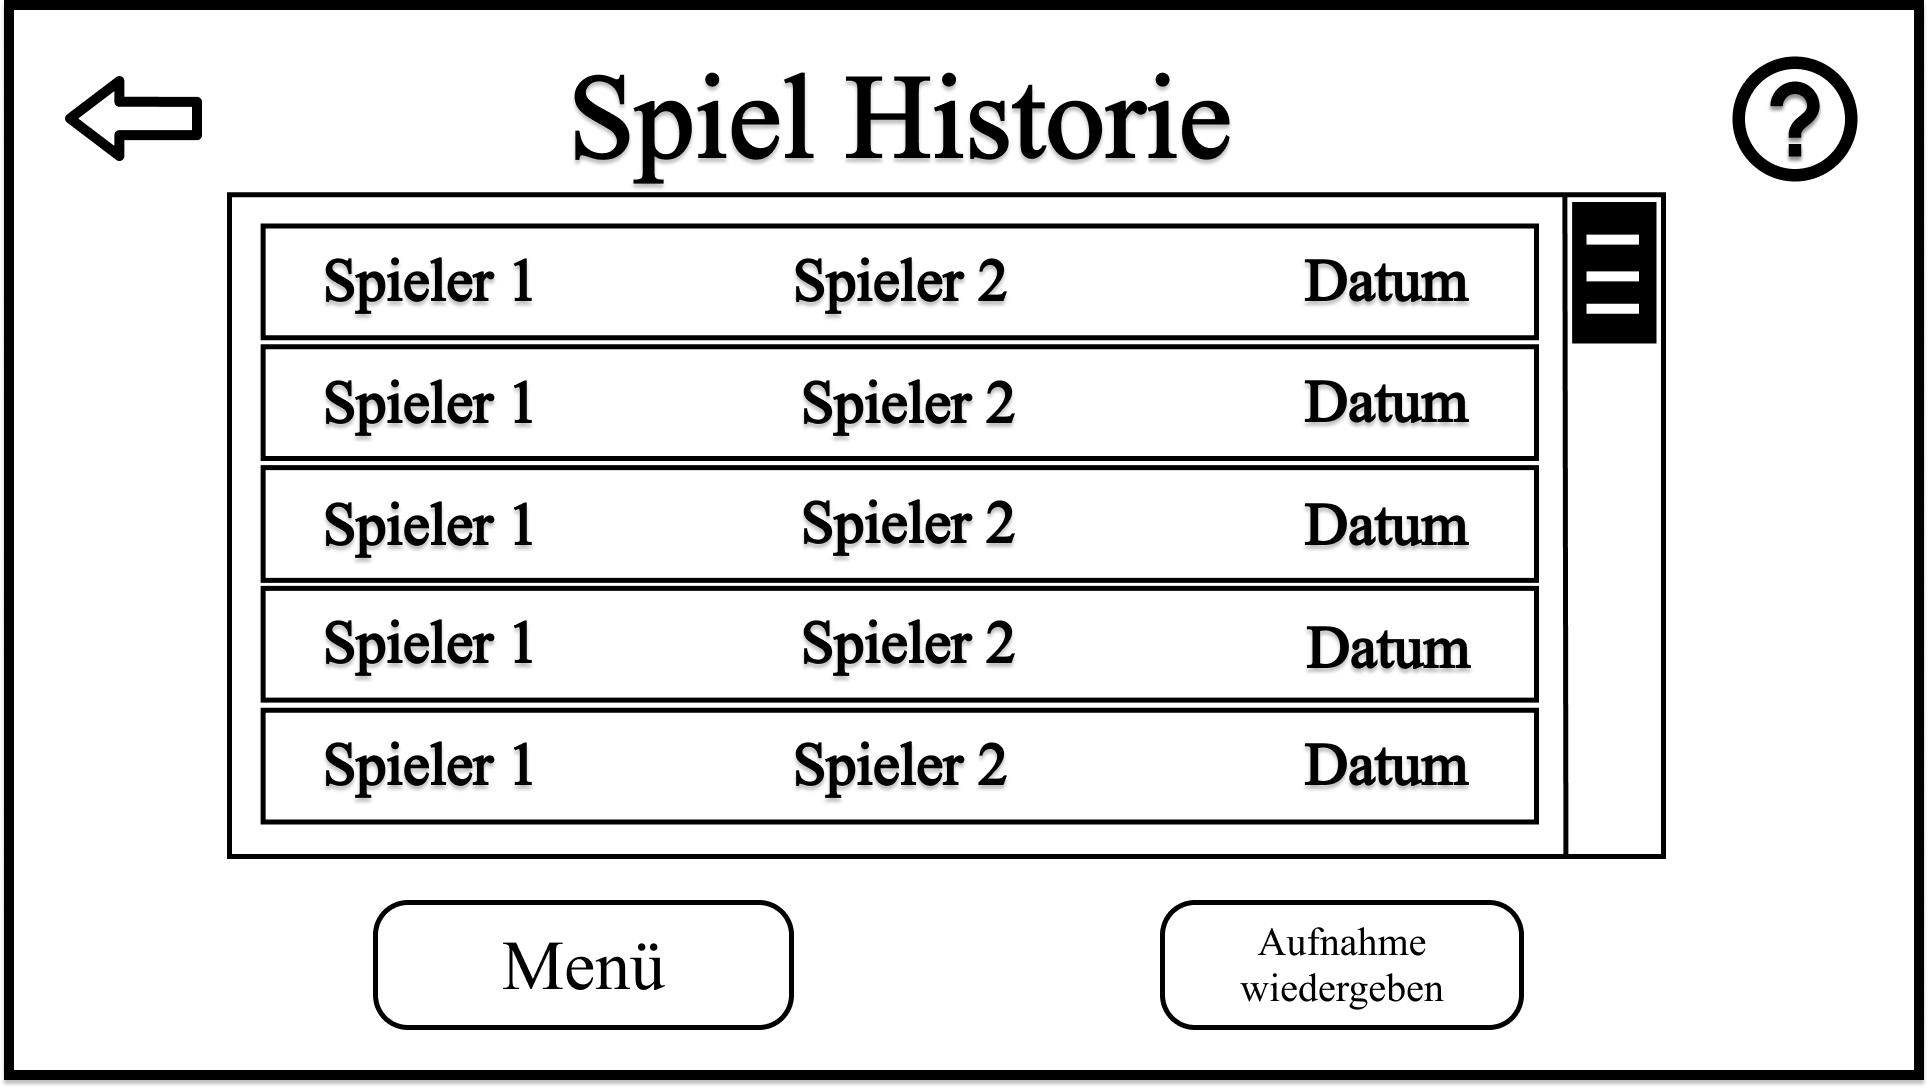
\includegraphics[width=\textwidth]{images/ReplayAbspielen}
\captionof{figure}{\textbf{ReplayAbspielen}:\\
Der Benutzer kann eine Spielaufzeichnung durch Anklicken auswählen und mit Klicken des Knopfes Aufnahmen wiedergeben die Wiedergabe starten. Durch Klicken des Knopfes Menü kann der Spieler in das Menü zurückkehren.
}

\includegraphics[width=\textwidth]{images/Aufzeichnung}
\captionof{figure}{\textbf{Aufzeichnung}:\\
Der Spieler kann die Aufzeichnung durch Klicken der Taste zurück in das Menü zurückkehren.
Zudem kann der Spieler mit dem runden Knopf die Aufzeichnung pausieren, und mit den Knöpfen rechts
und links davon die Aufzeichnung doppelt so schnell oder halb so schnell abspielen.
}

\includegraphics[width=\textwidth]{images/Zuschauen}
\captionof{figure}{\textbf{Zuschauen}:\\
Der Nutzer hat keine Möglichkeit das Spiel zu beeinflussen und schneller oder langsamer
abzuspielen. Der Nutzer kann lediglich alles sehen, was auch im Spiel sichtbar ist. Der Nutzer kann vom zuschauen Bildschirm in das Menü wechseln, indem er den Knopf
Menü klickt.
}

\includegraphics[width=\textwidth]{images/GreatHouseWahl}
\captionof{figure}{\textbf{GreatHouseWahl}:\\
Der Nutzer kann durch die Radiobuttons House 1 und House 2 eines der beiden Häuser markieren. Durch Selektieren des Buttons bestätigen
bestätigt der Spieler seine Auswahl. Wenn der Nutzer über ein definiertes Zeitintervall keine Auswahl bestätigt, wird die Partie abgebrochen.
Der Nutzer kehrt dann in die Lobby zurück.
}

\includegraphics[width=\textwidth]{images/Spielfeld}
\captionof{figure}{\textbf{Spielfeld}:\\
Der Dialog \glqq{}Spielfeld\grqq zeigt das aktuelle Spielfeld und den aktuellen Spielzustand an. Dafür sieht man in der Mitte das Spielfeld und auf der linken und rechten Seite jeweils die Statistiken der Spieler, das heißt zum Beispiel wie viel Spice der Spieler hat oder in welcher Runde sie sich befinden. Das ist auch die Oberfläche, die ein Zuschauer sehen kann. Wenn der Server die Charakterzugphase abhandelt, dann ändert sich der Dialog für den Spieler und der \glqq{}Spielfeld\grqq{}-Dialog wird zum \glqq{}Charakterzug\grqq{}-Dialog.
}

\includegraphics[width=0.8\textwidth]{images/Charakterzug}
\captionof{figure}{\textbf{Charakterzug}:\\
Im \glqq{}Charakterzug\grqq{}-Dialog hat der Benutzer die Möglichkeit seine Charakterzüge durchzuführen. Dafür wird quasi ein Overlay erzeugt, das heißt der Dialog des Spielfeldes wird erweitert für den Spieler, der am Zug ist. \\ Dann sieht der Spieler unten in einer Leiste alle auf der Karte platzierten Charakter und kann diese mit einem Klick (Kasten zeigt aktuelle Auswahl) auswählen. Die Leiste ist wie eine horizontale Scrollbar. Wenn der Spieler einen Charakter ausgewählt hat, dann sieht er an der linken Seite Informationen zu dem Charakter und zu dieser Phase. Das heißt wie viele MP und AP der Spieler noch hat und dieser Charakter verbrauchen würde. Außerdem existieren in diesem Abschnitt Buttons für die verschiedenen Aktionen, die man mit dem Charakter machen kann. \\ Wenn der Spieler den Charakter bewegen will, dann muss er mit der Maus auf das Feld des Charakters klicken und den Charakter an die gewünschte Stelle ziehen. Damit wird die Bewegung ausgeführt. 
}

\includegraphics[width=0.8\textwidth]{images/Spielmenü}
\captionof{figure}{\textbf{Spielmenü}:\\
Den \glqq{}Spielmenü\grqq{}-Dialog erreicht der Benutzter über das drücken der \glqq{}ESC\grqq{}-Taste. Hier hat der Benutzer die Möglichkeit die Partie zu pausieren oder zu verlassen.Über das Zahnrad kommt der Benutzer zu den Einstellungen. Der Dialog kann über den \glqq{}X\grqq{}-Knopf oder erneutes drücken der \glqq{}ESC\grqq{}-Taste geschlossen werden.
}

\includegraphics[width=0.7\textwidth]{images/Partie wurde pausiert}
\captionof{figure}{\textbf{Partie wurde pausiert}:\\
Zudem kann es passieren, dass man die Partie spielt und der gegnerische Mitspieler die Partie pausiert. Dann wird ebenfalls ein \glqq{}Pause\grqq{}-Dialog angezeigt, in dem der Spieler jedoch keine Interaktion vornehmen kann, sondern nur auf die Partiefortsetzung warten kann. 
}

\includegraphics[width=0.7\textwidth]{images/Partie pausiert}
\captionof{figure}{\textbf{Partie pausiert}:\\
Im \glqq{}Pause\grqq{}-Dialog hat der Spieler dann wieder die Möglichkeit, die Partie fortzusetzen, wofür es ebenfalls einen Button gibt. Dieser öffnet einen Bestätigungsdialog. Drückt der Benutzer in diesem Dialog \glqq{}Ja\grqq{}, dann wird das Spiel fortgesetzt und der Spieler kehrt zu dem \glqq{}Spielfeld\grqq{}-Dialog zurück.
}

\includegraphics[width=0.7\textwidth]{images/Rundenstatistik}
\captionof{figure}{\textbf{Rundenstatistik}:\\
Der Dialog \glqq{}Rundenstatistik\grqq{} stellt eine Art Hinweisfenster dar. In diesem Dialog wird dem Benutzer die aktuellen Ergebnisse der letztem Runde anzeigt, solange der Server die Runde beendet, die nächste vorbereitet und startet. Das heißt der Spieler sieht aktuelle Statistiken, wie in dem \glqq{}Sieg/Niederlage\grqq{}-Dialog.
}

\includegraphics[width=\textwidth]{images/end(lose)Screen}
\captionof{figure}{\textbf{end(lose)Screen}:\\
Im Endbildschirm wird dem Spieler bei einer Niederlage das Label Niederlage und bei einem Sieg das Label Sieg angezeigt.
Zudem werden dem Spieler hier die Statistiken beider Spieler angezeigt.
Durch Klicken der Taste Menü kommt der Spieler zurück in das Menü.
}

\includegraphics[width=\textwidth]{images/end(win)Screen}
\captionof{figure}{\textbf{end(win)Screen}:\\
Im Endbildschirm wird dem Spieler bei einer Niederlage das Label Niederlage und bei einem Sieg das Label Sieg angezeigt.
Zudem werden dem Spieler hier die Statistiken beider Spieler angezeigt.
Durch Klicken der Taste Menü kommt der Spieler zurück in das Menü.
}
\end{center}

\newpage

\subsection{Domänenmodell}
Dieser Abschnitt enthält das Domänenmodel, welches in fünf kleinere Modelle unterteilt wurde. Zu Beginn die Gesamtstruktur und darauf folgend die zugehörigen Teilmodelle.

\centering
\includegraphics[width=\textwidth]{images/DMMain}
\captionof{figure}{Domänenemodel: Gesamtstruktur (enthält Teilmodel: \ref{fig:dmcharaktere}, \ref{fig:dmszenario}, \ref{fig:dmrunde})}
\label{fig:dmmain}

\vspace{2cm}

\includegraphics[width=\textwidth]{images/DMCharaktere}
\captionof{figure}{Teilmodel: Häuser und Charaktere}
\label{fig:dmcharaktere}

\vspace{2cm}
\includegraphics[width=\textwidth]{images/DMSzenario}
\captionof{figure}{Teilmodel: Szenario}
\label{fig:dmszenario}

\vspace{2cm}
\includegraphics[width=\textwidth]{images/DMRunde}
\captionof{figure}{Teilmodel: Runde (enthält Teilmodel: \ref{fig:dmcharakterzug})}
\label{fig:dmrunde}

\vspace{2cm}

\includegraphics[width=\textwidth]{images/DMCharakterzug}
\captionof{figure}{Teilmodel: Charakterzug-Rundphase}
\label{fig:dmcharakterzug}

\vspace{2cm}
\includegraphics[width=\textwidth]{images/DMCharakterzug}
\captionof{figure}{Teilmodel: Charakterzug-Rundphase}
\label{fig:dmcharakterzug}

\newpage

\flushleft

\section{Randbedingungen}
\subsection{Qualität}

Es müssen folgende nicht-funktionalen Anforderungen an das gesamte System und die Entwickler erfüllt werden: 

\nfa{Robustheit}{Das gesamte System darf bei 100 Partien maximal einmal abstürzen. Das gesamte System stürzt genau dann ab, wenn eine Komponente des Systems abstürzt, das heißt aufgrund eines nicht behandelten Fehlers beendet wird.}{Das gesamte System soll robust sein, das heißt stabil laufen, weil der Benutzer spielen möchte und nicht ständig das Spiel neu starten oder warten will. Zudem nervt ein nicht stabiles System den Benutzer und vertreibt ihn damit möglicherweise.}{}{2}{\rref{A-Teilnehmer}}{QA-Robustheit}

\nfa{Zuverlässigkeit des Servers}{Der Server soll zuverlässig laufen. Das heißt, er soll eine Uptime von mindestens 95\% haben und innerhalb von 1 Minute neu gestartet werden können.}{Der Server ist für die Verwaltung der Spieler und der Partie zuständig und ist deshalb ein integraler Bestandteil der Anwendung. Daher sollte er zuverlässig und verfügbar sein.}{}{2}{\rref{A-Teilnehmer}}{QA-Zuverlässigkeit}


\nfa{Toleranz des Servers}{Der Server soll bei Verbindungsabbrüchen oder zu spät gesendeten oder nicht interpretierbaren Nachrichten des Clients tolerant sein. Das bedeutet, der Server schließt die Session bei einem Verbindungsabbruch nicht sofort. Außerdem wählt der Server bei zu spät gesendeten Nachrichten oder nicht interpretierbaren Nachrichten ein Standardverhalten. Der Client soll jedoch ebenfalls versuchen, das Problem zu beheben und zum Beispiel einen erneuten Verbindungsaufbau zu initiieren.}{Durch das tolerante Verhalten des Servers kann die Partie auch bei Problemen des Clients fortgesetzt werden und wird nicht jedes Mal abgebrochen, wenn zum Beispiel bei dem Client das WLAN ausfällt. Dies trägt zur Robustheit der Anwendung bei.}{\nfaref{QA-Robustheit}}{4}{\rref{A-Benutzer-Client}, \rref{A-Teilnehmer}}{QA-Toleranz}

\nfa{Plattformen}{Die Komponenten \textit{Benutzer-Client} und \textit{Editor} müssen auf einer aktuellen Version von Microsoft Windows oder einer aktuellen Debian Linux-Distribution (zum Beispiel Ubuntu) lauffähig sein. Die Komponenten \textit{KI-Client} und \textit{Server} müssen inklusive ihrer Abhängigkeit als Docker-Container lauffähig sein.}{Der \textit{Benutzer-Client} und der \textit{Editor} soll auf mehreren Betriebssystemen lauffähig sein, um eine möglichst große Zielgruppe zu erreichen und keine Anforderung an den Benutzer zu stellen. \textit{KI-Client} und \textit{Server} sollen als Docker-Container lauffähig sein, weil der Benutzer nicht direkt damit interagiert und die Docker-Images ohne komplizierte lokale Build-Prozesse direkt gestartet werden können. Damit erreicht man eine Unabhängigkeit von der Plattform und kann somit die Komponenten einfacher zum Laufen bekommen.}{\nfaref{QA-Portierbarkeit}}{5}{\rref{A-Tutor}}{QA-Plattform}

\nfa{Portierbarkeit}{Es muss möglich sein, die Anwendung auf andere Betriebssysteme zu portieren. Das bedeutet, dass innerhalb von 4 Arbeitswochen eines Teammitglieds, die Anwendung auf einem anderen Betriebssystem lauffähig sein sollte.}{Die Anwendung soll portierbar sein, weil sich nach der Entwicklung herausstellen könnte, dass die Benutzer ein anderes Betriebssystem bevorzugen und daher das Spiel auf dieser Plattform nutzen wollen.}{\nfaref{QA-Plattform}}{1}{\rref{A-Entwickler}, \rref{A-Teilnehmer}}{QA-Portierbarkeit}

\nfa{einfache Installation}{Die Anwendung sollte mithilfe eines Skripts oder einem Programm installiert werden können. Dieses Skript oder Programm nimmt dem Benutzer die typischen Aufgaben beim Installationsprozess, wie zum Beispiel das Herunterladen und Installieren von Abhängigkeiten, ab.}{Der Benutzer möchte das Spiel spielen und nicht die Zeit damit verbringen, das Spiel zunächst zum Laufen zu bekommen. Ein aufwendiger Installationsprozess könnte den Benutzer frustrieren.}{\nfaref{QA-Plattform}}{1}{\rref{A-Teilnehmer}}{QA-Installation}

\nfa{Testbarkeit}{Die Anwendung soll mit entsprechenden Tests, insbesondere mit Unit-Tests, geprüft werden. Diese Tests sollen zu 100\% erfüllt werden und mindestens 80\% des nicht automatisch generierten Source Codes abdecken. Diese Tests beziehen sich nicht auf die Benutzerschnittstelle. Zudem sollen die Tests automatisiert bei jedem Commit auf dem \textit{release}-Branch ausgeführt werden.}{Die Verwendung von Tests kann die Entwicklung des Codes vereinfachen, weil dann bei der Implementierung durch die Tests ein genaues Verständnis vorliegen muss, was der Code machen soll. Außerdem lassen sich so Fehler oder Bugs frühzeitig finden und die Qualität des Codes steigt.}{\nfaref{QA-Robustheit}, \nfaref{QA-Zuverlässigkeit}}{5}{\rref{A-Tutor}, \rref{A-Entwickler}}{QA-Testbarkeit}

\nfa{Bedienbarkeit}{Die Anwendung soll einfach und intuitiv sein. Das bedeutet, dass die Anwendung mithilfe des Benutzerhandbuchs innerhalb von 2 Stunden vom Benutzer bedient werden kann.}{Durch eine einfache Bedienbarkeit kann sich der Teilnehmer ganzheitlich auf das Spiel konzentrieren und wird nicht durch ein unübersichtliches Design vom Spiel abgehalten oder frustriert}{\nfaref{QA-Benutzerhandbuch}}{3}{\rref{A-Teilnehmer}}{QA-Bedienbarkeit}

\nfa{Programmiersprache}{Für die Entwicklung der Anwendung wird hauptsächlich die Programmiersprache \textsc{Java 11} verwendet. Die Bibliotheken sind frei wählbar. }{\textsc{Java} ist die Lehrsprache an der Universität Ulm und damit den Entwicklern und dem Auftraggeber bekannt. Außerdem wird SonarQube zur Analyse des Source Codes verwendet und die Anwendung benötigt \textsc{Java 11}.}{\nfaref{QA-DokumentationSourceCode}}{2}{\rref{A-Tutor}, \rref{A-Entwickler}}{QA-Programmiersprache}

\nfa{Dokumentation des Source Code}{Der Source Code soll verständlich dokumentiert werden. Dabei wird der Javadoc-Stil verwendet. Automatisch generierter Code, wie zum Beispiel getter-Methoden sollen nicht dokumentiert weren. 90\% des nicht automatisch erzeugten Codes sollen ausführlich dokumentiert werden.}{Das ist eine Vorgabe des Auftraggebers. Außerdem erleichtert die Dokumentation von Code, dass andere Personen (unabhängig, ob sie Entwickler sind oder nicht) dokumentierten Code leichter verstehen und weiterentwickeln können. Ebenso kann die Dokumentation des Codes bei der Entwicklung helfen, sich bewusst zu werden, was der Code machen soll oder bei späterer Weiterentwicklung, was der Code macht.}{\nfaref{QA-Programmiersprache}}{5}{\rref{A-Tutor}, \rref{A-Entwickler}}{QA-DokumentationSourceCode}

\nfa{Implementierungs- und Dokumentationssprache}{Der Source Code und die Dokumentation im Code, das heißt die Kommentare, müssen in Englisch verfasst werden.}{Das ist eine Vorgabe des Auftraggebers. Außerdem ist englisch die etablierte Sprache bei der Implementierung und der Dokumentation, weil dadurch der Code international verständlich ist.}{\nfaref{QA-DokumentationSourceCode}}{5}{\rref{A-Tutor}, \rref{A-Entwickler}}{QA-Dokumentationssprache}

\nfa{Sprache der Benutzerschnittstelle}{Die Texte der Benutzerschnittstelle werden auf Deutsch verfasst.}{Die Anwendung wird vor allem von Personen genutzt, deren Muttersprache deutsch ist und damit würde die englische Sprache wenig Vorteile bieten, jedoch eventuell Schwierigkeiten bei der Verständlichkeit hervorrufen.}{}{5}{\rref{A-Tutor}, \rref{A-Teilnehmer}}{QA-Sprache-Benutzerschnittstelle}

\nfa{Benutzerhandbuch}{Für die Anwendung soll ein Benutzerhandbuch bereitgestellt werden. Dieses Dokument wird auf Deutsch verfasst und soll dem Benutzer eine einfache Bedienung der Anwendung ermöglichen. In diesem Dokument sollen alle spiel-relevanten Informationen und Komponenten, sowie die Benutzerschnittstelle anhand von Beispielen erklärt werden.}{Ein Benutzerhandbuch kann die Bedienung einer Anwendung und den Einstieg in das Spiel erleichtern. Dies vermeidet Frust bei den Benutzern, weil sie die Anwendung nicht verstehen oder Probleme bei der Bedienung haben.}{\nfaref{QA-Bedienbarkeit}, \nfaref{QA-Sprache-Benutzerschnittstelle}}{5}{\rref{A-Tutor}, \rref{A-Teilnehmer}}{QA-Benutzerhandbuch}

\nfa{Dokumentation}{Der gesamte Entwicklungsprozess und auch das entstandene Produkt muss dokumentiert werden. Das bedeutet, dass Tests, Reviews und weitere Maßnahmen zur Qualitätssicherung dokumentiert werden müssen. Außerdem soll ein Projekttagebuch und ein Entwicklerhandbuch angelegt werden.}{Die Dokumentation ermöglicht nach und während der Entwicklung der Anwendung anderen Kunden, den Prozess zu beurteilen oder sich mit der Architektur und Umsetzung der Komponenten auseinanderzusetzen.}{\nfaref{QA-Testbarkeit}, \nfaref{QA-Dokumentationssprache}, \nfaref{QA-Projekttagebuch}, \nfaref{QA-Entwicklerhandbuch}}{5}{\rref{A-Tutor}, \rref{A-Entwickler}}{QA-Dokumentation}

\nfa{Projekttagebuch}{Es soll ein Projekttagebuch zum Erfassen der Tätigkeiten (zum Beispiel Implementierung oder Treffen) geführt werden}{Mit dem Projekttagebuch kann man später die Entwicklungsprozess nachvollziehen und ermitteln, wie viel jeder gearbeitet hat.}{\nfaref{QA-Dokumentation}}{5}{\rref{A-Tutor}, \rref{A-Entwickler}}{QA-Projekttagebuch}

\nfa{Entwicklerhandbuch}{Es soll ein Entwicklerhandbuch angelegt werden. Dieses Entwicklerhandbuch soll die Architektur und die implementierten Funktionen beschreiben, sowie die verwendeten Technologien auflisten und begründen.}{Das Entwicklerhandbuch anderen Entwicklern das die Qualität des System zu beurteilen. Besonders auf der Messe, wenn man andere Komponenten einkauft, kann das die Entscheidung vereinfachen.}{\nfaref{QA-Dokumentation}}{5}{\rref{A-Tutor}, \rref{A-Entwickler}}{QA-Entwicklerhandbuch}

\nfa{Dokumentations-Sprache}{Alle im Rahmen des Projekts, das heißt der Entwicklung der Anwendung, anfallenden Dokumente, wie zum Beispiel das Benutzerhandbuch werden auf Deutsch verfasst.}{Die Anwendung wird vor allem von Personen genutzt, deren Muttersprache deutsch ist und damit würde die englische Sprache wenig Vorteile bieten, jedoch eventuell Schwierigkeiten bei der Verständlichkeit hervorrufen. }{\nfaref{QA-Dokumentation}}{5}{\rref{A-Tutor}, \rref{A-Entwickler}}{QA-Dokumentationssprache}

\nfa{Kombinierbarkeit von Komponenten}{Die Komponenten: Server, Benutzer-Client, KI-Client und Editor sollen beliebig über Teamgrenzen hinweg kombinierbar sein.}{Dies ist nötig, um in einer späteren Phase des Projektes Komponenten auszutauschen.}{\faref{FA-Server}, \faref{FA-BC}, \faref{FA-KI},  \faref{FA-Spielkomponenten}}{5}{\rref{A-Tutor}, \rref{A-Entwickler}}{FA-Kombinierbarkeit-Komponenten}

\nfa{Versionskontrolle GitLab}{Der Entwicklungsprozess und der zu entwickelnde Code soll auf der Plattform GitLab versioniert werden und damit die Versionskontrolle Git zum Einsatz kommen. Dafür sollen Issues, Milestones und Boards verwendet werden, um den SCRUM-Prozess umsetzen sowie Commits und Branches, um den Code zu versionieren und zu strukturieren. Außerdem soll eine CI/CD-Pipeline verwendet werden, um automatisiert zu testen usw.}{Dies ist hilfreich bei der Zusammenarbeit von mehreren Personen an einem Projekt und der Verwaltung von Code. So kann man beispielsweise bei fehlgeschlagenen Features einfach wieder zurückspringen oder durch das automatische Testen Zeit sparen und trotzdem die Qualität sichern.}{}{5}{\rref{A-Tutor}, \rref{A-Entwickler}}{QA-Versionskontrolle}

\newpage

\flushleft

\subsection{Betriebskonzept}

Das Programm ist für Systeme mit Windows als Betriebssystem gedacht. Die Anwendung lässt den Benutzer das Spiel 'Dune' spielen. Hierbei kann entweder gegen einen echten Gegner oder eine KI gespielt werden, wobei auch laufenden Partien zugesehen werden kann. Es wird im Hauptmenü eine Hilfsoption mit Erklärungen zum Spielablauf geben.

\subsection{Entwicklungsvorgaben}

Das Softwaregrundprojekt wird von sechs Studenten geplant und implementiert. Der Entwicklungsprozess ist in Meilensteine unterteilt, welche die Projektphasen Analyse, Entwurf und Implementierung abdecken. Während des gesamten Prozesses steht das Team in Kontakt mit dem Vertreter des Auftraggebers (Tutor). Für die Implementierung wird die Entwicklungsumgebung IntelliJ und UnityHub benutzt und zur Versionsverwaltung ein GitLab-Repository verwendet. Der Programmcode wird in englischer Sprache kommentiert und mit Javadoc dokumentiert.

\subsection{Abnahmekriterien}

Kriterien für eine erfolgreiche Abnahme sind eine fristgerechte und korrekte Abgabe aller Team-Meilensteine mit einer ausreichenden Bewertung. Zudem wird vorausgesetzt, dass jedes Team-Mitglied n-1 der insgesamt n Einzelübungsblätter, fristgerecht abgegeben und bestanden hat.
Des Weiteren ist eine regelmäßige Anwesenheit und Mitarbeit im Tutorium notwendig und auch eine aktive Mitarbeit im Team, die durch das Projekttagebuch dokumentiert wird. Dazu gehört eine eigene Programmiertätigkeit in ausreichendem Umfang.
Voraussetzungen für eine erfolgreiche Abnahmesitzung zum Ende des Projekts sind die Vorlage einer lauffähigen Version der Software und die Umsetzung der Kernfunktionalität, also aller verbindlichen Anforderungen. Zudem ist eine gute Qualität der entwickelten Software mit einer sinnvollen Testabdeckung und nachgewiesen durch umfangreiche und dokumentierte Maßnahmen zur Qualitätssicherung erforderlich. Die Einhaltung des Scrum-Entwicklungsprozesses und die sinnvolle Verwendung des Team-Repository und Scrum-Board im GitLab sind ebenfalls erforderlich. Dazu gehört auch eine ordentliche Dokumentation der Software und des Projektverlaufs.
Die Abnahme ist dann erfolgreich, wenn der Kunde mit dem endgültigen Produkt zufrieden ist.


\newpage

\flushleft

\section{Architekturentwurf}

\subsection{Komponentendiagramm}
\label{ssec:Komponentendiagramm}
Das zu entwickelnde Spiel \textsc{Deserts of Dune} ist eine verteilte Anwendung und besteht aus vier großen Subsystemen (siehe \faref{FA-Spielkomponenten}). Diese Subsysteme sind die vier großen Komponenten (die auch ausgetauscht werden können), die wiederum aus einzelnen Teilsystemen bzw. Unterkomponenten bestehen. Die strukturelle Gliederung des gesamten Systems von dem Spiel ist in den folgenden Komponentendiagrammen visualisiert und begründet. 

\vspace{0.7cm}

\begin{center}
\includegraphics[width=0.95\textwidth]{images/Komponentendiagramm-Gesamtübersicht}
\captionof{figure}{Komponentendiagramm des Gesamtsystems. Dabei kann man die Gesamtstruktur erkennen, sowie die Gliederung des Benutzer-Clients in die graphische Anzeige und den Controller. Diese grobe Architektur wurde von den Auftraggebern festgelegt und im Benutzer-Client bietet sich eine Aufteilung in graphische Anzeige und Controller an, damit man das MVC-Pattern umsetzt, was bei der Testbarkeit und Entwicklung Vorteile bietet.}  

\includegraphics[width=0.95\textwidth]{images/Komponentendiagramm-Netzwerk}
\captionof{figure}{Komponentendiagramm des Moduls \textit{Netzwerk}. Da das Spiel eine verteilte Anwendung ist, müssen die einzelnen Systeme über ein Netzwerk kommunizieren und benötigen daher jeweils ein Modul, das die Schnittstelle zur Außenwelt darstellt und die ausgetauschten Daten in für die Komponenten entsprechend lesbare Nachrichten umwandelt.}  


\includegraphics[width=0.95\textwidth]{images/Komponentendiagramm-Editor}
\captionof{figure}{Komponentendiagramm des Editors. Dieses wurde jedoch nur angedeutet, da der Editor nicht von Team 08 entwickelt wird, sondern später eingekauft wird und somit nicht modelliert werden muss.}  

\includegraphics[width=0.95\textwidth]{images/Komponentendiagramm-KI-Client}
\captionof{figure}{Komponentendiagramm des KI-Clients. Der KI-Client beinhaltet vor allem eine Komponente, die die Züge vorschlägt, da dieser keine Visualisierung oder Eingaben benötigt, sondern nur das Spiel spielen muss.}  

\includegraphics[width=0.95\textwidth]{images/Komponentendiagramm-GUI}
\captionof{figure}{Komponentendiagramm der graphischen Anzeige bzw. der GUI. Dabei muss die GUI nicht nur das Spielfeld und alle sonstigen Informationen darstellen, sondern auch mit Nutzereingaben umgehen können, weswegen eine Komponente für die Darstellung (Aufteilung in 2D und 3D, da dies verschiedene Implementierungen benötigt) und eine für die Eingaben zuständig ist. Außerdem müssen die Eingaben verarbeitet werden das Spiel korrekt dargestellt, worum sich eine Spiellogik kümmert. \\ Diese Komponente ist dem Subsystem \textit{Benutzer-Client zugeordnet}}  

\includegraphics[width=0.95\textwidth]{images/Komponentendiagramm-Server}
\captionof{figure}{Komponentendiagramm des Servers. Der Server muss wie in den funktionalen Anforderungen (siehe \autoref{ssec:fas}) die Konfigurationen laden, die Clients verwalten und die Partie abwickeln. Da diese Aufgaben weitestgehend voneinander unabhängig ausgeführt werden können, sollte man diese in eigene gekapselte Komponenten auslagern. Bei der Partieabwicklung kann man sogar die Welt (= Model), und die Abhandlung der Runden (= Controller) voneinander trennen, was die Testbarkeit und Implementierung vereinfacht.}

\end{center}

\vspace{0.5cm}

Im Folgenden ist die Zuordnung der funktionalen Anforderungen aus \autoref{ssec:fas} und den Komponenten zu erkennen. Dabei wird für jede Komponente des Systems (siehe Komponentendiagramme oben) aufgelistet, welche Anforderung sie abgedeckt: \\ 
\begin{tabularx}{\linewidth}{l|X}
	\textbf{Komponente} & \textbf{zugeordnete Anforderungen} \\
	\hline
	Gesamtarchitektur & \mfaref{FA-Architektur}, \mfaref{FA-Spielkomponenten}\\
	Editor & \mfaref{FA-Editor}, \mfaref{FA-Spielbrett} - \mfaref{FA-Feldart-Gebirge}, \mfaref{FA-Konfiguration}, \mfaref{FA-LadenUndModifizieren}- \mfaref{FA-ZufälligeSzenariokonfiguration}\\
	KI-Client & \mfaref{FA-KI}, \mfaref{FA-Start-KI}\\
	KI-Komponente & \mfaref{FA-Pausierung-KI} - \mfaref{FA-Intelligenzstufen}\\
	Netzwerk-Komponente & \mfaref{FA-Netzwerkprotokoll} - \mfaref{FA-Spielprotokoll}, \mfaref{FA-Server-Clientverbindung}, \mfaref{FA-Server-Erlaube-Zuschauer} - \mfaref{FA-Server-verspätete-Nachrichten}, \mfaref{FA-Server-Session-offen-halten}, \mfaref{FA-Verbindungsaufbau-BC}, \mfaref{FA-Verbindungsaufbau-KI}\\
	Server & \mfaref{FA-Server}, \mfaref{FA-Docker-Server}, \mfaref{FA-Server-Protokollverletzung}, \mfaref{FA-FormatKonfiguration}\\
	Konfigurations-Handler & \mfaref{FA-ServerlädtSzenario}, \mfaref{FA-Server-Partie-Konfiguration}\\
	Client-Handler & \mfaref{FA-Spieleranzahl}, \mfaref{FA-Beobachtung}, \mfaref{FA-Server-Information-Spielzustand}, \mfaref{FA-Registrierung-Spieler}, \mfaref{FA-Registrierung-Zuschauer}, \mfaref{FA-Einbindung-KI}\\
	Partie-Handler & \mfaref{FA-Abstand-Felder} - \mfaref{FA-gleichwertige-Alternativen}, \mfaref{FA-Server-Partiebeginn}, \mfaref{FA-Server-Partiepause}, \mfaref{FA-Server-Siegbedingung}, \mfaref{FA-ReplayLog}, \mfaref{FA-Pausierung-BC}\\
	Benutzer-Client & \mfaref{FA-BC}, \mfaref{FA-Vereinfachung-Spielinteraktion}\\
	Graphische Anzeige & \mfaref{FA-Replay}\\
	GUI & \mfaref{FA-Visualisierung-Spiel}, \mfaref{FA-Spielinteraktion}\\
	Spielfeld & \mfaref{FA-Sichtbarkeit-Spielfeld}, \mfaref{FA-Visualisierung-Spielgeschehen}, \mfaref{FA-Visualisierung-Aktion}, \mfaref{FA-Visualisierung-Phasen}, \mfaref{FA-Visualisierung-Spielausgang}\\
	HUD & \mfaref{FA-Sichtbarkeit-Inventar}, \mfaref{FA-Visualisierung-Spielstatus}, \mfaref{FA-Visualisierungsdauer}\\
\end{tabularx}

\vspace{0.5cm}

\subsection{Implementierungsentwurf}
Im Folgenden ist der Implementierungsentwurf ausgeführt. Das heißt für jede in \autoref{ssec:Komponentendiagramm} angegebene Komponente und wird nun erläutert, wie diese Komponente implementiert werden soll. Damit wird die grobe Sicht auf das System, gegebenen durch die Komponentendiagramme und die Domänenmodelle verfeinert. \\ Dabei sind die Klassendiagramme auch entsprechend der Komponenten aufgeteilt. Zu den Klassendiagramme folgen gegebenenfalls noch Erklärungen zu den Klassen und den Methoden, insofern diese nicht selbsterklärend sind \footnote{Als selbsterklärend werden beispielsweise Aufzählungsklassen (gekennzeichnet mit \textit{<<enum>>}), Konstrukturen oder aussagekräftige Methoden angesehen}. Am Ende jeden Abschnitts findet sich die Zuordnung der Methoden zu den funktionalen Anforderungen aus \autoref{ssec:fas}, die sie implementieren und umsetzen. \\ 

\subsubsection{KI-Client}
\begin{center}
\includegraphics[width=0.95\textwidth]{images/KI-Client-Klassendiagramm}
\label{fig:KI-Client-Klassendiagramm}
\captionof{figure}{Übersicht über die Klassen, die der KI-Client voraussichtlich beinhalten wird. Da zu dem aktuellen Zeitpunkt die genaue Logik bzw. Strategie, die der KI-Client verwenden wird um zu spielen, noch nicht endgültig festgelegt wurde, sind diese Klassen möglichst generisch gehalten. Zudem verwendet der KI-Client für die Simulation des Spiels und Validierung der Züge die \textit{shared logic}}
\end{center}
\paragraph{Main}
Da der KI-Client eine eigenständige Komponente von \textsc{Deserts of Dune} sein wird, muss diese Komponente auch gestartet werden und dafür einen Einstiegspunkt haben. Dafür bietet sich eine \class{Main} an. Mithilfe der \method{main} kann der der KI-Client dann gestartet werden, wobei der Start in der Konsole stattfindet und entsprechende Parameter als Argumente übergeben werden. Um den Client dann zu starten, wird die \method{startAiClient} aufgerufen, die entweder mit dem entsprechend implementieren Netzwerkcontroller (\class{NetworkController} aus Netzwerk-Paket) oder einem schnellen Interface (\class{FastServerInterface}) eine Verbindung zu dem Server aufbaut.
\paragraph{FastServerInterface}
Diese Klasse realisiert eine schnelle Verbindung zum Server. Normalerweise kommuniziert der KI-Client über das Netzwerk mit dem Server. Da diese Kommunikation über die WebSockets aber langsam ist und man beim Training des KI-Clients viele Spiele in kurzer Zeit spielen will, muss der KI-Client auch eine direkte Verbindung zum Server haben. Mithilfe der \method{connectToServer} und \method{disconnectFromServer} kann der KI-Client direkt eine Instanz vom Server erstellen bzw. zerstören, sich mit dem Server verbinden oder trennen und dann schneller mit dem Server kommunizieren. Diese findet dann mithilfe der \method{sendMessage} und \method{receiveMessage} statt, welche die Funktionalität von den Methoden aus dem Netzwerkmodul nachahmen. 
\paragraph{GameSimulator}
Diese Klasse spielt oder simuliert eine Partie, in der der KI-Client gegen einen anderen Client spielt. Dafür kann das Spiel mit der \method{playGame} gespielt werden, wie es ein menschlicher Spieler in dem Benutzer-Client ebenso macht. Dafür wird mithilfe der \method{findBestMove} der beste Zug ermittelt. Die Implementierung und das Verhalten der Methode ist noch nicht festgelegt. Generell wird jedoch in dieser Methode mit der \method{simulateGame} das Spiel vor simuliert (das heißt alle erlaubten Züge gespielt und und am Ende wieder rückgängig gemacht) und die möglichen Stellungen bewertet. Dafür muss die \method{doEvaluate} aus dem Interface \textit{Evaluation} implementiert werden. Dann wird anhand der Bewertung der beste Zug ausgewählt und dem Server mitgeteilt. Am Ende der Partie kann diese noch gespeichert werden, was ein Replay ermöglicht (durch \method{saveGame} realisiert). Dafür wird jede Nachricht in einem String gespeichert und dieser in eine Textdatei gespeichert. 
\paragraph{GameDB}
Die \class{GameDB} repräsentiert eine Art Datenbank für die gespielten und gespeicherten Spiele. Da diese Datenbank nur einmal benötigt wird, implementiert diese Klasse das Singleton-Pattern durch die \method{getInstance}. Mithilfe der \method{getGames} kann man dann später die Partie wieder anfordern und gegebenenfalls nochmal wiedergeben oder für das Training einsetzen. 
\paragraph{Game}
Diese Klasse repräsentiert eine gespielte Partie, indem dort der Verweis auf die entsprechende Textdatei mit dem Nachrichtenverlauf der Partie gespeichert ist. Diese Datei kann mithilfe der \method{readReplayFile} gelesen werden. Diese Methode liest dann diese Datei wieder aus und speichert die Nachrichten wieder in einem String. Mit der \method{replayGame} kann dieser String dann verwendet werden, um die Nachrichten darin Stück für Stück zu analysieren und an den Server zu senden. Damit kann das Spiel nochmal abgespielt werden
\paragraph{World}
Diese Hilfs-Klasse repräsentiert eine Welt, in der Szenario und alle Charaktere gespeichert sind. Diese dient der Simulation der nächsten Züge aus der \class{GameSimulator}. Denn mit der \method{changeWorld} kann ein Zug simuliert werden, indem diese fiktive Welt entsprechend den Spielregeln verändert wird,  ohne dabei das richtige Spielfeld vom Server zu verändern. Mit der \method{getAvailableMoves} können alle nach den Spielregeln erlaubten Züge angefragt werden, um einen Spielbaum zu erstellen. Dafür wird jeder mögliche Zug generiert und überprüft, ob dieser erlaubt ist.

\begin{tabularx}{\linewidth}{l|X}
	\textbf{funktionale Anforderung} & \textbf{Methode(n), die diese umsetzt} \\ \hline
	\mfaref{FA-KI} & \textit{playGame}, \textit{simulateGame}, \textit{findBestMove}, \textit{doEvaluate} \\ 
	\mfaref{FA-Replay} & \textit{saveGame}, \textit{readReplayFile}, \textit{replayGame} \\ 
	\mfaref{FA-Start-KI} & \textit{main}, \textit{startAIClient} (\textit{connectToServer}) \\ 
	\mfaref{FA-Verbindungsaufbau-KI} & \textit{startAIClient} (\textit{connectToServer}) \\
	\mfaref{FA-Pausierung-KI} & \textit{playGame} \\
	\mfaref{FA-Zugwahl-KI} & \textit{playGame}, \textit{simulateGame}, \textit{findBestMove}, \textit{doEvaluate} \\ 
	\mfaref{FA-Zugdauer-KI} & \textit{findBestMove} \\ 
	\mfaref{FA-Intelligenzstufen} & \textit{Difficulty-enum}, \textit{findBestMove}, \textit{doEvaluate} \\
	\mfaref{FA-Einbindung-KI} & \textit{main} \\
\end{tabularx}

\vspace{0.5cm}

\subsubsection{Netzwerk-Modul}
Im Folgenden sind die Klassendiagramme zu sehen, die das Netzwerk-Modul umfasst. Diese Klassen müssen allen Komponenten zugänglich sein, jedoch werden manche Klassen spezifisch von jeder Komponente erweitert oder genauer implementiert. \\ 

\begin{center}
\includegraphics[width=0.95\textwidth]{images/Netzwerk-Util-Klassendiagramm}
\label{fig:Netzwerk-Util-Klassendiagramm}
\captionof{figure}{Übersicht über die Hilfs-Klassen aus dem Netzwerk-Modul. Diese Paket beinhaltet vor allem Aufzählungsklassen, Parser sowie Klassen, die die Informationen von Netzwerk-Nachrichten kapseln. Diese Klassen müssen von allen Komponenten des Systems verwendet werden können.}

\includegraphics[width=0.95\textwidth]{images/Netzwerk-Messages-Klassendiagramm}
\label{fig:Netzwerk-Messages-Klassendiagramm}

\includegraphics[width=0.95\textwidth]{images/Netzwerk-Messages-Klassendiagramm 2}
\label{fig:Netzwerk-Messages2-Klassendiagramm}

\includegraphics[width=0.95\textwidth]{images/Netzwerk-Messages-Klassendiagramm 3}
\label{fig:Netzwerk-Messages3-Klassendiagramm}
\captionof{figure}{Übersicht über die Klassen, die die Nachrichten gemäß des Standardisierungsdokuments darstellen. Diese können gegebenenfalls nochmal angepasst werden, müssen aber auch von allen Komponenten verwendet werden.}
\end{center}

\includegraphics[width=0.95\textwidth]{images/Netzwerk-Netzwerkcontroller-Klassendiagramm}
\label{fig:Netzwerk-Netzwerkcontroller-Klassendiagramm}
\captionof{figure}{Übersicht über die Klassen, die die Kommunikation der Subsysteme über das Netzwerk ermöglichen. Dabei sind vor allem die Controller entscheidend, die die Nachrichten verarbeiten. Diese Klassen müssen ebenso in allen Komponenten verwendet werden können, jedoch muss die \class{NetworkController} je nach Komponente unterschiedlich implementiert werden, da dies der übergeordnete Controller ist, der die Kommunikation leitet und die Komponenten zum Beispiel verschiedene Netzwerkendpunkte sind.}

\paragraph{MessageConverter}
Der \textit{MessageConverter} ist eine statische Klasse, die dem umwandeln von Nachrichten und Strings dient. Dafür wird ein JSON-Parser verwendet, der die Nachrichten, die als Objekte vorliegen, in JSON-Strings umwandelt und umgekehrt. Dafür sind ist die \method{fromMessage} (wandelt ein Nachrichten-Objekt in den entsprechenden String um) und die \method{toMessage} (wandelt den JSON-String in das passende Nachrichten-Objekt um) verfügbar.

\paragraph{CommandLineParser}
Diese Klasse dient dem auswerten der Parameter, die in der Kommandozeile eingegeben werden können. Diese Klasse dient also dem Zweck, die Parameter die beim Start des Servers oder des KI-Client über die Kommandozeile übergeben werden, zu verarbeiten und die Befehle umzusetzen. Dafür gibt es einerseits die \method{printHelp}, die alle Parameter und ihre Bedeutung in der Konsole ausgibt und die \method{parseArgument}, die ein Parameter bekommt und die entsprechenden Befehle umsetzt. Das bedeutet, dass zum Beispiel bei dem Parameter, der dafür steht die Hilfe anzufordern, alle Befehle mit deren Erklärungen (durch die \method{printHelp}) auszugeben oder durch den entsprechenden Parameter der Port des Servers in \textit{ConnectionsHandler} gesetzt wird. 

\paragraph{Response}
Diese Hilfs-Klasse dient als Antwort für gesendete Nachrichten über das Netzwerk. Das heißt, wenn eine Nachricht empfangen wird und der entsprechende Controller diese verarbeitet, wird ein \textit{Response} zurückgegeben, der angibt ob die Verarbeitung erfolgreich war oder sonst den Fehler als String. 

\paragraph{Position}
Die \class{Position} ist eine Hilfs-Klasse, die eine x- und eine y-Koordinate speichert und somit eine Position auf dem Spielfeld repräsentieren kann. Diese Kapselung ist sinnvoll, weil in manchen Nachrichten Position versendet werden. Eine Position kann bewegt werden, wenn sich ein Charakter zum Beispiel bewegt, was durch die \method{move} umgesetzt wird. 

\paragraph{CharacterStatistics}
Diese Hilfs-Klasse speichert die Statistiken eines Characters, da diese ebenfalls über das Netzwerk versendet werden können. Dafür werden in dem Objekt die Statistiken in den entsprechenden Attributen gespeichert. Diese Klasse dient alleine dem Zweck, Informationen zu speichern. 

\paragraph{MapField}
Die Klasse \textit{MapField} repräsentiert ein einziges Teil aus dem Spielfeld. Diese Klasse beinhaltet keine Funktionalität, da sie nur die Informationen über ein Teil des Spielfeldes speichern muss (Position, Feldtyp, Spice und ob es in einem Sandsturm ist), da diese Klasse nur verwendet wird um Änderungen des Spielfeldes über das Netzwerk mitzuteilen. 

\paragraph{Message}
Die \class{Message} ist eine abstrakte Message, die sozusagen das Grundgerüst jeder Nachricht darstellt. Das heißt, dass jede Nachrichtem-Klasse von dieser Klasse erbt und somit eine Version und einen Typ hat (siehe Standardisierungsdokument). Der Typ von jeder Nachricht kann mit der \method{getMessageType} abgefragt werden, um die Nachricht zu klassifizieren. Die in \autoref{fig:Netzwerk-Messages-Klassendiagramm} aufgezeigten Nachrichten-Klasse erben direkt von dieser Klasse und haben somit keine weitere Gemeinsamkeiten. Alle aufgelisteten Nachrichten-Klassen implementieren eine Nachricht aus dem Standardisierungsdokument. 

\paragraph{ClientServerMessage}
Diese Klasse ist eine Erweiterung der \class{Message} und ist die Vorlage für weitere Klassen, weshalb sie auch abstrakt ist. Die von dieser Klasse erbenden Klassen halten weiter eine Client-ID, um bei der Kommunikation über das Netzwerk den Adressaten oder Sender eindeutig identifizieren zu können. Wieder implementieren alle erbenden Nachrichten-Klassen (siehe \autoref{fig:Netzwerk-Messages2-Klassendiagramm}) die entsprechenden Nachrichten aus dem Standardisierungsdokument. 

\paragraph{TurnMessage}
Diese Klasse ist nochmal eine Erweiterung der \class{ClientServerMessage} und ist eine abstrakte Vorlage für alle Nachrichten-Klassen, die auch noch eine Charakter-ID speichern müssen, weil sie eine Nachricht repräsentieren, die in Zusammenhang mit einem Charakter oder eine Spielentität stehen, die eindeutig identifiziert werden muss. Wieder implementieren alle erbenden Nachrichten-Klassen (siehe \autoref{fig:Netzwerk-Messages3-Klassendiagramm}) die entsprechenden Nachrichten aus dem Standardisierungsdokument.

\paragraph{MessageFactory}
Die statische Klasse \textit{MessageFactory} setzt das Factory-Pattern um und ermöglicht es, Nachrichten-Objekte zu erstellen. Dafür wird mithilfe der \method{createMessage} eine Nachricht erstellt, indem der gewünschte Typ angegeben wird und die Argumenten für die Nachricht in einem Array. Die Methode erstellt dann Objekt der entsprechenden Nachricht. 

\paragraph{ConnectionHandler}
Der \textit{ConnectionHandler} ist für die Umsetzung des Netzwerkendpunkts zuständig. Das heißt diese Klasse implementiert den WebSocket und sorgt für den Verbindungsaufbau und die Kommunikation über das Netzwerk. Dafür gibt es die Methoden \textit{onOpen}, \textit{onClose}, \textit{onMessage} und \textit{onError}, die implementieren, was beim Verbindungsaufbau und -abbau passiert sowie bei Fehlern oder dem Erhalt einer Nachricht. 

\paragraph{MessageReceiver}
Diese Klasse sorgt für die Verwaltung der eingehenden Nachrichten. Dafür gibt es eine Schlange, die alle eingehenden Nachrichten speichert, damit diese später weiterverarbeitet werden können. Mit der \method{receiveMessage} können dann Nachrichten \glqq empfangen\grqq{} werden und der Warteschlange hinzugefügt werden, die dann mit der \method{parseMessage} nacheinander ausgewertet werden. 


\paragraph{MessageEmitter}
Diese Klasse sorgt für die Verwaltung der ausgehenden Nachrichten. Dafür gibt es eine Schlange, die alle ausgehenden Nachrichten speichert, damit diese nacheinander geparsed und abgesendet werden können. Mit der \method{sendMessage} können die Nachrichten dann \glqq versendet\grqq{} werden, wobei diese vorher mit der \method{parseMessage} in das entsprechende UTF-8 JSON-Format gebracht werden müssen. 

\paragraph{NetworkController}
Der \textit{NetworkController} ist übergeordnete Verwaltungseinheit der Netzwerkkomponente. Er hält Implementierungen der Klassen \textit{ConnectionHandler}, \textit{MessageReceiver} und \textit{MessageEmitter}, sowie einen \textit{MessageController}. Damit kann der \textit{NetworkController} die eingehenden und ausgehenden Nachrichten, die Verbindung zu den anderen Netzwerk-Clients und die 
Nachrichten an sich verwalten und auswerten. Mit der \method{handleSendingMessage} werden dann zu sendende Nachrichten verarbeitet und gesendet und mit der \method{handleReceivedMessage} eingehende Nachrichten verarbeitet. Diese Methoden sind die, die von der entsprechenden Komponenten zugänglich sind und verwendet werden, um über das Netzwerk zu kommunizieren. Die anderen Klassen und Methoden werden kann von diesem \textit{NetworkController} verwaltet. 

\paragraph{MessageController}
Die \class{MessageController} ist der Controller, der die Logik enthält, die beim Erhalt oder beim Senden einer Nachricht ausgeführt werden soll. Durch die Aufteilung in diesen Controller und die Nachrichten-Klassen (Model) wird das MVC-Pattern implementiert. Der \textit{MessageController} implementiert dann die Interfaces \textit{iReceivedMessageHandler} und \textit{iEmittedMessageHandler}, die alle Methoden enthalten, die die Controller für eingehende und zu sendende Nachrichten repräsentieren. \\ Der \textit{MessageController} wird von weiteren Controllern erweitert, um je nach Komponenten und Implementierung des Netzwerk-Moduls verschiedene Controller-Funktionalitäten umzusetzen. Jeder Controller muss jedoch Debug-Nachrichten versenden und handlen können, was durch die Methoden \textit{onDebugMessage} und \textit{doDebug} umgesetzt wird.
\\ Generell sind die Methoden mit dem Namen \textit{on<Nachrichtenname>} dafür da, eingehende Nachrichten zu verarbeiten und die Logik zu implementieren, die bei Erhalt der entsprechenden Nachricht auszuführen ist. Die Methoden mit dem Namen \textit{do<Nachrichtenname>} beinhalten die Logik, die ausgeführt werden soll, wenn eine bestimmte Nachricht versendet werden soll. \\ Dabei gibt es weitere speziellere Controller, die den \textit{MessageController} erweitern. So verwendet der Server die \class{ServerMessageController}, welche alle Methoden beinhaltet, die notwendig sind um alle Nachrichten zu empfangen und zu versenden, die der Server laut dem Standardisierungsdokument verarbeiten muss. Die \class{ClientMessageController} umfasst alle Methoden, die jeder Client braucht, wobei diese einmal von der \class{SpectatorMessageController} erweitert wird (Klasse, die der Benutzer-Client des Zuschauers verwendet) und von der \class{PlayerMessageController}. Diese Klasse beinhaltet alle Methoden, die die Nachrichten verarbeiten, die die mitspielenden Clients versenden und empfangen müssen. Dabei gibt es weiterhin eine Unterteilung in die Klassen \textit{HumanPlayerMessageController} und \textit{AIPlayerMessageController}, die der Benutzer-Client für den Spieler und der KI-Client beinhalten. Diese Aufteilung besteht, da der menschliche Spieler mehr Nachrichten versenden kann (zum Beispiel Antrag auf Pausierung) als der KI-Client und somit auch einen erweiterten Controller benötigt, der diese zusätzliche Logik umsetzen kann. 

\begin{tabularx}{\linewidth}{l|X}
	\textbf{funktionale Anforderung} & \textbf{Methode(n), die diese umsetzt} \\ \hline
	\mfaref{FA-Netzwerkprotokoll} & \textit{onOpen}, \textit{onClose}, \textit{onMessage}, \textit{onError} \\	
	\mfaref{FA-Kodierung} & \textit{fromMessage}, \textit{toMessage} \\
	\mfaref{FA-Nachrichtenformat} & \textit{fromMessage}, \textit{toMessage} \\ 
	\mfaref{FA-Spielprotokoll} & \textit{alle Methoden der MessageController bzw. die der Interfaces} \\  
	\mfaref{FA-Docker-Server} & \textit{parseArgument} \\ 
	\mfaref{FA-Start-KI} & \textit{parseArgument} \\ 
\end{tabularx}

\vspace{2cm}


Im Folgenden ist die Zuordnung der funktionalen Anforderungen aus Unterabschnitt 2.3 und den
Klassendiagrammen zu erkennen. Dabei wird für die wichtigen Klassen und jedes Diagramms aufgelistet, welche Anforderungen es abdeckt:
\begin{tabularx}{\linewidth}{l|X}
	\textbf{Klassendiagramm Charaktere und Häuser} & \textbf{zugeordnete Anforderungen} \\
	\hline
	Charaktere & \mfaref{FA-Sichtbarkeit-Spielfeld},  \mfaref{FA-Feldart-Düne},   \mfaref{FA-Heilung-Charakter},   \mfaref{FA-Lautheit-Charakter},   \mfaref{FA-Aktion-Angriff},  \mfaref{FA-Aktion-Spice-Aufsammeln},  \mfaref{FA-Aktion-Spice-Hoarding},   \mfaref{FA-Aktion-Voice},   \mfaref{FA-Spezielle-Aktion},   \mfaref{FA-Aktion-Kanly}, \mfaref{FA-Mentat},  \mfaref{FA-Normale-Aktion},  \faref{FA-Charaktere},  \mfaref{FA-Aktion-Angriff},  \mfaref{FA-Aktion-Spice-Aufsammeln} \\
	Häuser & \mfaref{FA-GreatHouses}, \mfaref{FA-Haus-Corrino}, \mfaref{FA-Haus-Atreides}, \mfaref{FA-Haus-Harkonnen},  \mfaref{FA-Haus-Ordos}, \mfaref{FA-Haus-Richese}, \mfaref{FA-Haus-Vernius} \\
\end{tabularx}
\vspace{0.5cm}


\begin{tabularx}{\linewidth}{l|X}
	\textbf{Klassendiagramm Szenario und Felder} & \textbf{zugeordnete Anforderungen} \\
	\hline
	Feld & \mfaref{FA-Höhenniveau}, \mfaref{FA-Feld}, \mfaref{FA-Feldarten}, \mfaref{FA-Betretbarkeit}, \mfaref{FA-Feldart-Stadt}, \mfaref{FA-Feldart-Flachsand}, \mfaref{FA-Feldart-Düne}, \mfaref{FA-Feldart-Felsplateau}, \mfaref{FA-Feldart-Gebirge} \\
	Szenario & \mfaref{FA-Spielbrett}, \mfaref{FA-Abstand-Felder}, \mfaref{FA-Sichtbarkeit-Inventar}, \mfaref{FA-Sichtbarkeit-Spielfeld} \\
\end{tabularx}
\vspace{0.5cm}


\begin{tabularx}{\linewidth}{l|X}
	\textbf{Klassendiagramm Charakterzug-Rundphase} & \textbf{zugeordnete Anforderungen} \\
	\hline
	Charakterzug-Rundphase & \mfaref{FA-Charaktere}, \mfaref{FA-Runden und Züge}, \mfaref{FA-Charakterzug-Rundenphase},  \mfaref{FA-Charakterzug}, \mfaref{FA-Charakterzug} \\
	CharakterZug & \mfaref{FA-Charakterzug}, \mfaref{FA-Aktionen}, Bewegungsschritt \\
	Bewegungsschritt & \mfaref{FA-Charakterzug}, \mfaref{FA-Bewegungsrichtung-Charakter},  \mfaref{FA-Drängeln-Charakter}, \mfaref{FA-Bewegung-Charakter} \\
	Aktion & \mfaref{FA-Aktionen}, \mfaref{FA-Spezielle-Aktion}, \mfaref{FA-Normale-Aktion} \\
	SpezielleAktion & \mfaref{FA-Spezielle-Aktion}, \mfaref{FA-Aktion-Kanly}, \mfaref{FA-Aktion-FamiliyAtomics}, \mfaref{FA-Aktion-Spice-Hoarding}, \mfaref{FA-Aktion-Voice}, \mfaref{FA-Aktion-Sword-Spin}, \mfaref{swordspin}, \mfaref{voice}, \mfaref{kanly}, \mfaref{familyatomics}, \mfaref{spicehoarding} \\
	NormaleAktion & \mfaref{FA-Normale-Aktion}, \mfaref{FA-Aktion-Angriff}, \mfaref{FA-Aktion-Spice-Aufsammeln}, \mfaref{FA-Aktion-Spice-Übergeben} \\
\end{tabularx}
\vspace{0.5cm}

\begin{tabularx}{\linewidth}{l|X}
	\textbf{Klassendiagramm Runde} & \textbf{zugeordnete Anforderungen} \\
	\hline
	Runde (ohne FA's von Charakterzug) & \mfaref{FA-Aktion-Spice-Blow}, \mfaref{FA-Dünenwanderung}, \mfaref{FA-Phase-Dünenwanderung}, \mfaref{FA-Zellulärer-Automat}, \mfaref{FA-Sandsturm}, \mfaref{FA-Phase-Sandsturm}, \mfaref{FA-Sandwurm}, \mfaref{FA-Phase-Sandwurm}, \mfaref{FA-Phase-Klon} \\
\end{tabularx}
\vspace{0.5cm}

\begin{tabularx}{\linewidth}{l|X}
	\textbf{Klassendiagramm network} & \textbf{zugeordnete Anforderungen} \\
	\hline
	MessageConverter & \mfaref{FA-Netzwerkprotokoll}, \mfaref{FA-Kodierung}, \mfaref{FA-Spielprotokoll} \\
	ConnectionHandler &  \mfaref{FA-Server-Clientverbindung}, \mfaref{FA-Server-Verbindungstrennung}, \mfaref{FA-Server-Session-offen-halten}, \mfaref{FA-Server-Protokollverletzung}, \mfaref{FA-Verbindungsaufbau-BC}, \mfaref{QA-Toleranz} \\
	MessageEmitter & \mfaref{FA-Server-Erlaube-Zuschauer}, \mfaref{FA-ReplayLog}, \mfaref{FA-Server-Information-Spielzustand} \\
	MessageReceiver & \mfaref{FA-Server-ClientInput} \\
	ClientMessageController & \mfaref{FA-Server-ClientInput} \\
	HumanMessageController & \mfaref{FA-Registrierung-Spieler},  \\
	SpectatorMessageController & \mfaref{FA-Registrierung-Zuschauer}, \mfaref{FA-Beobachtung} \\
	AIMessageController & \mfaref{FA-Verbindungsaufbau-KI}, \mfaref{FA-Zugdauer-KI} \\
\end{tabularx}
\vspace{0.5cm}


\begin{tabularx}{\linewidth}{l|X}
	\textbf{Klassendiagramm AI} & \textbf{zugeordnete Anforderungen} \\
	\hline
	Main & \mfaref{FA-Verbindungsaufbau-KI}, \mfaref{FA-Intelligenzstufen}, \mfaref{FA-Start-KI}  \\
	Difficulty & \mfaref{FA-Intelligenzstufen} \\
	FastServerInterface &  \mfaref{FA-Server-ClientInput}, \mfaref{FA-Server-Information-Spielzustand} {FA-Verbindungsaufbau-KI} \\
	GameSimulator & \mfaref{FA-Zugwahl-KI}, \mfaref{FA-FormatKonfiguration} \\
	World & \mfaref{FA-Spielbrett}, \mfaref{FA-Charaktere} \\
	Game & \mfaref{FA-ReplayLog}, \mfaref{FA-Replay} \\
\end{tabularx}
\vspace{0.5cm}

\begin{tabularx}{\linewidth}{l|X}
	\textbf{Klassendiagramm UserClient} & \textbf{zugeordnete Anforderungen} \\
	\hline
	MenuScene & \mfaref{FA-Registrierung-Spieler}, \mfaref{FA-Registrierung-Zuschauer}, \mfaref{FA-Verbindungsaufbau-BC} \\
	GameScene & \mfaref{FA-Visualisierung-Spielstatus}, \mfaref{FA-Visualisierung-Spielgeschehen}, \mfaref{FA-Visualisierung-Spiel}, \mfaref{FA-Visualisierung-Phasen}, \mfaref{FA-Visualisierung-Aktion}, \mfaref{FA-Visualisierung-Phasen}, \mfaref{FA-Visualisierung-Spielausgang}, \mfaref{FA-Visualisierungsdauer}, \mfaref{FA-Spielinteraktion}, \mfaref{FA-Vereinfachung-Spielinteraktion}, \mfaref{FA-Pausierung-BC}, \mfaref{FA-Replay} \\
\end{tabularx}
\vspace{0.5cm}

\begin{tabularx}{\linewidth}{l|X}
	\textbf{Klassendiagramm Configuration} & \textbf{zugeordnete Anforderungen} \\
	\hline
	ConfigurationParser & \mfaref{FA-Server-Partie-Konfiguration}, \mfaref{FA-ServerlädtSzenario}, \mfaref{FA-LadenUndModifizieren} \\
	Configuration & \mfaref{FA-ZufälligeSzenariokonfiguration}, \mfaref{FA-Szenariokonfiguration}, \mfaref{FA-Partiekonfiguration} \\
	PartyConfiguration & \mfaref{FA-FormatKonfiguration}, \mfaref{FA-Parameter-Partiekonfiguration}, \mfaref{FA-Partiekonfiguration} \\
	ScenarioConfiguration & \mfaref{FA-FormatKonfiguration}, \mfaref{FA-Szenariokonfiguration}, \mfaref{FA-Parameter-Szenariokonfiguration} \\
\end{tabularx}
\vspace{0.5cm}


\end{document}
